\chapter{Schéma de programmation dynamique pour résoudre SMEPC}
\minitoc
\newpage
\label{SMEPC_programmation}
\section{Introduction}

Ce chapitre présente un schéma de programmation dynamique (DPS) pour résoudre le problème \textbf{SMEPC}, nous désignons par \textbf{DPS\_SMEPC} ce DPS \cite{ChrMinTot81tsptw}. %\cite{RePEc:inm:oropre:v:35:y:1987:i:2:p:266-273}.
  La \textbf{section} \ref{algo_SMEPC} aborde l'architecture du DPS du problème \textbf{SMEPC} et les pseudo-codes de ce dernier. La \textbf{section} \ref{Rounding_filter} présente un schéma d'approximation polynomiale du problème \textbf{SMEPC}. La \textbf{section} \ref{regles_de_filtrage} liste les mécanismes de filtrage du schéma de programmation dynamique \textbf{DPS\_SMEPC}. Ces mécanismes de filtrage permettront de diminuer le nombre d'états présents à un temps au sens de la programmation dynamique. On mesurera l'impact de ces mécanismes de filtrage sur le nombre d'états du \textbf{DPS\_SMEPC}. La \textbf{section} \ref{Experimentations_num} présente les résultats expérimentaux réalisés sur le \textbf{DPS\_SMEPC}. Pour conclure, la \textbf{dernière section} synthétise ce chapitre.


\section{Un algorithme de programmation dynamique pour SMEPC : DPS\_SMEPC}
\label{algo_SMEPC}
On présente le schéma de programmation dynamique nommé \textbf{DPS\_SMEPC} conçu pour calculer la solution optimale d'une instance du problème \textbf{SMEPC}. On explique son architecture et sa mise en œuvre algorithmique.
%\subsection{Architecture du DPS\_SMEPC}
Pour présenter l'architecture du problème \textbf{SMEPC}, on présente d'abord l'espace temps au sens de la programmation dynamique et les variables qui forment un état au sens de la programmation dynamique. Ensuite, on liste l'ensemble des décisions qui peuvent être prises à partir d'un état connu. Enfin, on écrit tous les états qui peuvent résulter de chaque décision ainsi que les coûts de transition et les pré-conditions à respecter pour qu'un état soit généré.
\subsection{ Espace temps et états}
L'espace temps de notre DPS est l'ensemble $\mathcal{T}$ des couples $(i, j), i = 0, \dots, N, j = 0, \dots, M + 1$ qui représentent le temps au sens de la programmation dynamique, fourni avec son ordre partiel standard. Nous pouvons étendre cet ordre partiel à un ordre linéaire de plusieurs façons, en associant à chaque couple $(i, j) \in \mathcal{T} $ (qui représente le temps au sens de la programmation dynamique) un successeur $Succ_{\Delta}(i,j)$. Par exemple, en fixant :

% $Succ_{\Delta}(i,j) =(i+1,j)$ si $i \leq N-1$ et $Succ_{\Delta}(i,j) =(0,j+1)$ sinon.
$$
Succ_{\Delta}(i,j)= \left\{
\begin{array}{ll}
(i+1,j) & \mbox{si  $i \leq N-1$.} \\
(0,j+1) & \mbox{sinon.}
\end{array}
\right.
$$

Nous relions les périodes $i$ et les stations $j$ en introduisant des relations ($<<$, $>>$, $==$) qui expriment le positionnement relatif d'une période $i$ et la date $T$ où le véhicule se trouve à la station $j$. C'est-à-dire que nous fixons pour tout $i \in \{0, \dots, N-1\}$ et $T \in \{0, \dots, TMax\}$ :
\begin{itemize}[label=$\square$]
	\item $T<<i$ si $T < p \times i$ ;
	\item $T>>i$ si $T\geq p \times (i+1)$ ;
	\item $T==i$ si $p \times i \leq T < p \times (i+1)$.
\end{itemize}

Ces relations vont nous aider à définir les variables d'état du \textbf{DPS\_SMEPC}. Pour tout couple $(i, j) \in \mathcal{T}$ qui représente le temps au sens de la programmation dynamique, on associe un état défini par un quadruplet $s = (Z, T, V^{Tank}, V^{Veh})$, avec :

\begin{itemize}[label=$\square$]
	\item $Z$ : l'état de la micro-usine de production d'hydrogène ;
	$$
	Z= \left\{
	\begin{array}{ll}
	1 & \mbox{si la micro-usine est active à la fin de la période $i-1$.} \\
	0 & \mbox{sinon.}
	\end{array}
	\right.
	$$
	\item $V^{Tank} $ : la quantité d'hydrogène dans la citerne à la micro-usine au début de la période $i$ ;
	
	\item $V^{Veh} $ : la quantité d'hydrogène dans le réservoir du véhicule lorsqu'il arrive à la station $j$ ;
	
	\item $T \in 0, \dots, TMax$ est une date signifiant :
	\begin{itemize}
		\item Si $T >> i$ alors le véhicule est en route vers la station $j$ et il y arrivera à la date $T$ (Voir figure (\ref{positions_vehicule})) ;
		\item Si $T<<i$ alors le véhicule est entre la station $j$ et la micro-usine. Le véhicule peut être entrain d'attendre à la micro-usine pour être rechargé (Voir figure (\ref{positions_vehicule})) ;
		\item Si $T==i$ alors le véhicule se trouve à la station $j$, et doit choisir entre aller à la station $j+1$ ou aller à la micro-usine se recharger (Voir figure (\ref{positions_vehicule})).
	\end{itemize}
\end{itemize}
\begin{figure}[H]
	\centerline{
		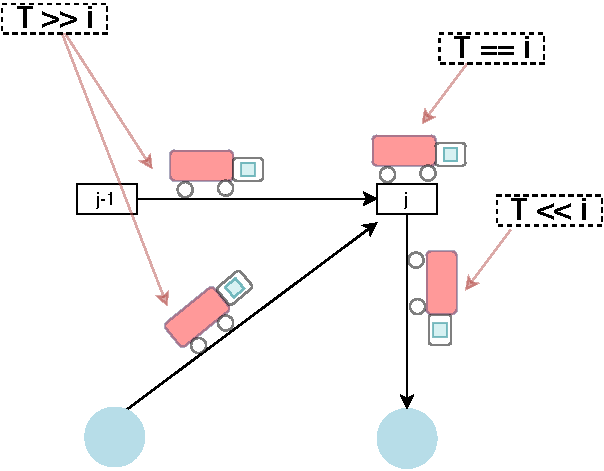
\includegraphics[height=8cm]{images_these/positions_vehicule.pdf}}
	\caption[Positionnements relatifs du véhicule par rapport à une station]{Le véhicule parcourt 3 positionnements relatifs possibles en fonction de $i$ et $j$ : soit le véhicule est en route vers la station $j$ ($i<<T$), soit le véhicule est à la station $j$ ($i==T$), soit le véhicule est entre la station $j$ et la micro-usine ($i>>T$).}
	\label{positions_vehicule}
\end{figure}
\begin{Rem}
	\label{Remarque_position_veh}
	Nous voyons que selon cette explication, le positionnement relatif de $T$ et $i$ par rapport aux relations $==$, $<<$ et $>>$ agit comme une variable d'état implicite, ce qui nous aidera à identifier les décisions qui peuvent être associées à un couple courant $(i, j) \in \mathcal{T}$ (qui représente le temps au sens de la programmation dynamique) et un état courant $s$, ainsi que leur impact. 
\end{Rem}
On vient de donner la signification de chaque variable d'un état au sens de la programmation dynamique du \textbf{DPS\_SMEPC}. De plus, on a décrit le temps au sens de la programmation dynamique du \textbf{DPS\_SMEPC}. On va maintenant donner la signification de chaque variables de décisions.
\subsubsection{Etat initial et Etats finaux}
L'état initial correspond au couple $(0,0)$ et au quadruplet $s_0=(0,0,H_0,E_0)$. Le couple $(0,0)$ représente le temps initial au sens de la programmation dynamique. On commence la tournée à la date $i=0$ et au dépôt initial ($j=0$), avec une micro-usine qui ne produit pas de l'hydrogène ($Z=0$). La date $T$ d'arrivé à la station $j=0$ est 0. $H_0$ est la quantité d'hydrogène initialement présente dans la citerne de la micro-usine. $E_0$ est la quantité d'hydrogène initialement présente dans le réservoir du véhicule.

L'état final correspond au couple $(i\leq N, M+1)$, qui représente le temps au sens de la programmation dynamique à l'état final, et à tout quadruplet $(Z,T\leq TMax, V^{Tank}\geq H_0, V^{Veh}\geq E_0)$ car la tournée finit au dépôt final $M+1$. Lorsque le véhicule finit sa tournée, la quantité d'hydrogène dans le réservoir du véhicule et la quantité d'hydrogène dans la citerne de la micro-usine doivent respectivement être au moins égale à $E_0$ et $H_0$. On veut ici éviter les stratégies triviales qui consistent à ne pas produire et à ne pas recharger tout au long de la tournée.
\subsection{Variables de décision}	

Une décision $D$ relative à un couple $(i, j) \in \mathcal{T}$ qui représente le temps au sens de la programmation dynamique et un état $s = (Z, T, V^{Tank}, V^{Veh})$ est un triplet $D = (z, x, \delta )$ dans $\{0, 1\}^3$, signifiant :

\begin{itemize}[label=$\square$]
	\item $z=1 $ signifie que la micro-usine produit de l'hydrogène pendant la période $i$ alors qu'elle ne produisait pas de l'hydrogène à la période $i-1$ ;
	$$
	z= \left\{
	\begin{array}{ll}
	1 & \mbox{si la micro-usine est active à la fin de la période i} \\
	0 & \mbox{sinon.}
	\end{array}
	\right.
	$$
	\item $x$ désigne une décision prise dès que $T == i$ : 
	
	$$
	x= \left\{
	\begin{array}{ll}
	1 & \mbox{si le véhicule se recharge en hydrogène à la micro-usine en se déplaçant de j à j + 1.} \\
	0 & \mbox{ s'il se déplace de la station $j$ à la station $j + 1$ sans se recharger.}
	\end{array}
	\right.
	$$
	%dans ce cas, $x = 0$ signifie que le véhicule se déplace de la station $j$ à la station $j + 1$ sans se recharger en hydrogène ; et $x = 1$ signifie qu'il se recharge en hydrogène à la micro-usine en se déplaçant de $j$ à $j + 1$. Dans le cas où $x = 0$, la transition induite transformera $j$ en $j' = j + 1$ et $i$ en $i' = i + 1$, sauf dans le cas où $T + t_j == i$ : dans ce dernier cas, aucune décision réelle n'est prise en ce qui concerne la production et $z$ est égal à 0 par défaut. Si ($T == i$) est faux alors $x$ devient non pertinent, on dit que $x$ est \textbf{neutralisée} et sa valeur est par défaut égale à 0, aucune transition n'y étant associée. 
	
	\item $\delta=1 $ signifie que le véhicule est à la micro-usine et décide de faire le plein de son réservoir d'hydrogène durant la période $i$. \textbf{On suppose que la recharge dure une période complète et en interdisant à la micro-usine d'être active pendant cette période}.
	
	
	$$
	\delta= \left\{
	\begin{array}{ll}
	1 & \mbox{si le véhicule décide de se recharger durant la période $i$} \\
	0 & \mbox{sinon.}
	\end{array}
	\right.
	$$
	
\end{itemize}
\begin{Def}
	Une variable de décision est neutralisée lorsqu'elle ne prend aucune valeur.
\end{Def}
Les variables de décisions décrites ci-dessus nous permettront de lister par la suite l'ensemble des décisions possibles. On a $2^3=8$ décisions au total, parmi lesquels cinq sont réalisables. Les trois décisions non réalisables sont :
\begin{itemize}[label=$\square$]
	\item $z=0$, $x=1$, $\delta=1$ : cette décision est interdite car lorsqu'on prend la décision de se recharger ($x=1$) le véhicule ne se trouve pas encore à la micro-usine mais à la station $j$. Et pour se déplacer de $j$ à la micro-usine, il faut au moins $d_j>0$ temps au véhicule. Le véhicule ne se recharge pas à la période $i$ parce que la recharge dure une période et le seul endroit où il se recharge c'est à la micro-usine ;
	\item $z=1$, $x=0/1$, $\delta=1$ : ces décisions sont interdites car on interdit que la production et la recharge se fassent simultanément pour éviter des pannes du système.
\end{itemize}	
Pour chaque décision possible, on va lister ses conditions de faisabilité appelées ici \textbf{pré-conditions}.
\subsection{ Pré-conditions, transitions et coûts liés aux décisions et aux états}
\label{liste_decisons}
Une décision est prise à la fin d'une période $i - 1$. Nous allons maintenant considérer le couple $(i, j) \in \mathcal{T}$ qui représente le temps au sens de la programmation dynamique, un état courant $s = (Z, T, V^{Tank}, V^{Veh})$, et analyser l'ensemble de toutes les décisions possibles $D = (z, x, \delta)$ en fonction de la position du véhicule par rapport à la station $j$. Pour chacune de ces décisions $D$, nous allons détailler les conditions qui assureront la faisabilité de $D$, la transition qui en résulte $((i, j), s)$ $\rightarrow$ $((i', j'), s')$ et le coût $CT$ de cette transition. Le trois positions possibles du véhicule par rapport à la station $j$ sont :



\textit{\textbf{Pour le cas}} $T>>i$ :

Le véhicule est en route vers la station $j$ et il y arrivera à la date $T$ (Voir figure (\ref{positions_vehicule})). Les variables de décisions $x$ et $\delta$ sont neutralisées. On a deux décisions possibles : produire durant la période $i$ ($z=1$) ou ne pas produire durant la période $i$ ($z=0$). Plus précisément :
\begin{enumerate}[label=\arabic*)]
	\item $z=1$ : la micro-usine produit de l'hydrogène pendant la période $i$. Pour que cette décision soit prise, la condition $V^{Tank} + R_i \leq C^{Tank}$ doit être vérifiée. C'est-à-dire qu'en produisant pendant la période $i$, la quantité d'hydrogène dans la citerne ne dépasse pas la capacité maximale de la citerne. Concernant l'évolution du temps au sens de la programmation dynamique on passe du couple $(i,j)$ au couple $(i+1,j)$. L'état résultant est $s'=(1, T,V^{Tank} + R_i, V^{Veh} )$ et le coût de transition est $Cost^F \times (1-Z) + Cost_i^V$.
	
	\item $z=0$ : la micro-usine ne produit pas de l'hydrogène pendant la période $i$. Cette décision est toujours possible. Concernant l'évolution du temps au sens de la programmation dynamique on passe du couple $(i,j)$ au couple $(i+1,j)$. L'état résultant est $s'=(0,T, V^{Tank},V^{Veh})$ et le coût de transition est nul.
\end{enumerate}



\textit{\textbf{Pour le cas}} $T<<i$ :

le véhicule est entre la station $j$ et la micro-usine (figure (\ref{positions_vehicule})) ou entrain d'attendre à la micro-usine pour se recharger. On a deux cas possible suivant que le véhicule arrive à la micro-usine avant ou au début de la période $i$ (i.e. $T+d_j\leq p\times i$) ou après le début de la période $i$ (i.e. $T+d_j>p\times i$).

\begin{enumerate}
	
	\item \underline{\textbf{1\ier{cas}}} $T+d_j\leq p\times i$ : le véhicule arrive à l'usine avant le début de la période $i$.
	La variable $x$ est neutralisée. On a trois décisions possibles : produire durant la période $i$ et faire attendre le véhicule à la micro-usine ($z=1$, $\delta=0$) ou ne pas produire durant la période $i$ et faire attendre le véhicule à la micro-usine ($z=0$, $\delta=0$) ou ne pas produire durant la période $i$ et recharger le véhicule durant la période $i$ ($z=0$, $\delta=1$). Plus précisément :
	\begin{enumerate}[label=\arabic*)]
		\item $z=1$, $\delta=0$ : la micro-usine produit de l'hydrogène pendant la période $i$ et le véhicule attend à la micro-usine pour se recharger. Les pré-conditions suivantes doivent être vérifiées :
		\begin{itemize}[label=$\square$]
			\item $V^{Tank} + R_i \leq C^{Tank}$ ;
			\item $p \times (i+1) +p+d^*_{j+1} + \sum_{k\geq j+1}t_k \leq TMax$ : le véhicule peut attendre à la micro-usine s'il a encore suffisamment de temps pour se recharger à la période suivante (il sortira alors de l'usine à la date $p \times (i+1) +p$), puis pour se déplacer de la micro-usine à la station $j+1$ ($d^*_{j+1}$) et enfin pour finir la tournée en supposant qu'il n'a pas d'autres recharges à effectuer ($\sum_{k\geq j+1}t_k$).
		\end{itemize}
		Concernant l'évolution du temps au sens de la programmation dynamique on passe du couple $(i,j)$ au couple $(i+1,j)$. L'état résultant est $s'=(1, T,V^{Tank} + R_i, V^{Veh} )$ et le coût de transition est $Cost^F \times (1-Z) + Cost_i^V$.
		
		\item $z=0$, $\delta=0$ : la micro-usine ne produit pas de l'hydrogène pendant la période $i$ et le véhicule attend à la micro-usine pour se recharger.
		Pour que la décision $\delta= 0$ soit réalisable, le véhicule doit avoir suffisamment de temps pour attendre, c'est-à-dire $p \times (i+1) +p+d^*_{j+1} + \sum_{k\geq j+1}t_k \leq TMax$.
		Concernant l'évolution du temps au sens de la programmation dynamique on passe du couple $(i,j)$ au couple $(i+1,j)$. L'état résultant est $s'=(0,T, V^{Tank},V^{Veh})$ et le coût de transition est nul.
		
		
		\item $z=0$, $\delta=1$ : la micro-usine ne produit pas de l'hydrogène pendant la période $i$ et le véhicule décide de se recharger à la période $i$.	
		\textbf{On suppose que la recharge dure une période et en interdisant à la micro-usine d'être active pendant cette période}. Cela signifie que $T << i$ et que la différence $p.i - T$ est au moins égale au temps nécessaire au véhicule pour passer de $j$ à la micro-usine car le véhicule doit être à la micro-usine pour pouvoir se recharger.
		
		Soit $Tour\_\_ = \varepsilon^*_{j + 1} +\sum_{ k \geq j + 1} e_k + E_0$ la quantité d'hydrogène nécessaire au véhicule pour partir de la micro-usine et finir la tournée en supposant qu'il n'a pas d'autres recharges à effectuer après la station $j$. Soit $Q\_Rech$ la quantité d'hydrogène rechargée par le véhicule durant la période $i$.
		
		La pré-condition suivante doit être vérifiée :
		\begin{itemize}[label=$\square$]
			
			\item $\varepsilon_{j+1} + \varepsilon^*_{j+1} \leq Inf(C^{Veh}, V^{Tank}+V^{Veh}-\varepsilon_j)$ : la quantité d'hydrogène dans le réservoir du véhicule après la recharge doit être au moins égale à la quantité d'hydrogène nécessaire pour aller en $j+1$ et revenir à la micro-usine.
		\end{itemize}
		
		Concernant l'évolution du temps au sens de la programmation dynamique on passe du couple $(i,j)$ au couple $(i+1,j+1)$. L'état résultant est $s'= (0, p\times (i + 1) + d^*_{j + 1}, V^{Tank}-Q\_Rech, V^{Veh} +Q\_Rech -\varepsilon_j-\varepsilon_{j+1}^*)$. Le coût de transition est $\alpha \times (p \times(i+1)+d^*_{j+1}-T)$.
		
		Concernant la quantité rechargée par le véhicule durant la période $i$, on a trois possibilités :
		\begin{itemize}[label=$\square$]
			\item Soit le véhicule vide la citerne, ce qui signifie qu'il a suffisamment de place dans son réservoir pour stocker l'hydrogène contenu dans la citerne, auquel cas $Q\_Rech = V^{Tank}$ ;
			\item Soit le véhicule remplit son réservoir, ce qui signifie que la citerne contient suffisamment d'hydrogène pour remplir le réservoir du véhicule, auquel cas $Q\_Rech = C^{Veh} - V^{Veh} + \varepsilon_j$ ;
			\item Soit le véhicule recharge exactement ce dont il a besoin pour partir de la micro-usine et finir la tournée en supposant qu'il n'a pas d'autres recharges à effectuer après la station $j$, auquel cas $Q\_Rech = Sup(0, Tour\_\_ - V^{Veh} + \varepsilon_j)$.
		\end{itemize}
		Donc, la quantité rechargée est $Q\_Rech = Inf(V^{Tank}, C^{Veh} - V^{Veh} + \varepsilon_j, Sup(0, Tour\_\_ - V^{Veh} + \varepsilon_j))$ car on veut éviter de recharger trop d'énergie alors que le véhicule n'en a pas besoin pour finir la tournée.
	\end{enumerate}
	\item \underline{\textbf{2\ieme{cas}}} $T+d_j>p\times i$ : le véhicule se déplace de la station $j$ à la micro-usine et il ne peut pas encore se recharger pendant la période $i$ car il arrive à la micro-usine à une date appartenant à la période $]i,i+1[$
	
	Les variables de décisions $x$ et $\delta$ sont neutralisées. On a deux décisions possibles : produire durant la période $i$ ($z=1$) ou ne pas produire durant la période $i$ ($z=0$). Plus précisément :
	\begin{enumerate}[label=\arabic*)]
		\item $z=1$ : la micro-usine produit de l'hydrogène pendant la période $i$. La pré-condition $V^{Tank} + R_i \leq C^{Tank}$ doit être vérifiée. Concernant l'évolution du temps au sens de la programmation dynamique on passe du couple $(i,j)$ au couple $(i+1,j)$. L'état résultant est $s'=(1, T,V^{Tank} + R_i, V^{Veh} )$ et le coût de transition est $Cost^F \times (1-Z) + Cost_i^V$.
		\item $z=0$ : la micro-usine ne produit pas de l'hydrogène pendant la période $i$. Cette décision est toujours possible. Concernant l'évolution du temps au sens de la programmation dynamique on passe du couple $(i,j)$ au couple $(i+1,j)$. L'état résultant est $s'=(0,T, V^{Tank},V^{Veh})$ et le coût de transition est nul.
	\end{enumerate}
	
\end{enumerate}




\textit{\textbf{Pour le cas}} $T==i$ :

Le véhicule est à la station $j$ et il doit choisir entre aller à la station $j+1$ ou aller à la micro-usine se recharger ( figure (\ref{positions_vehicule})). Dans ce cas, on a trois ou quatre décisions possibles. En effet, on a 2 décisions sont possibles quand le véhicule décide d'aller se recharger ($x=1$) : la micro-usine produit pendant la période $i$ ou ne produit pas en $i$. Par contre, quand le véhicule décide de continuer sa tournée vers la station $j+1$, le nombre de décisions dépendent de sa date d'arrivée à la station $j+1$ : 
\begin{itemize}[label=$\square$]
	\item Si le véhicule arrive à la station $j+1$ pendant la période $i$ alors la décision de production à la période $i$ est \textbf{remise à plus tard}. $z$ est donc neutralisé ;
	\item Si le véhicule arrive à la station $j+1$ après la fin de la période $i$ alors deux décisions sont possibles : la micro-usine produit pendant la période $i$ ou ne produit pas en $i$.
\end{itemize}
\begin{enumerate}
	\item $x=1$ : le véhicule décide de partir se recharger à la micro-usine ;
	
	\textbf{Pour ces deux décisions suivantes, la pré-condition suivante doit être satisfaite} :
	
	\begin{itemize}[label=$\square$]
		\item $Sup(p \times (i+1), T+d_j) +p+d^*_{j+1} + \sum_{k\geq j+1}t_k \leq TMax$ : le véhicule va à la micro-usine s'il a encore suffisamment de temps pour se recharger, pour se déplacer de la micro-usine à la station $j+1$ ($d^*_{j+1}$) et pour finir la tournée en supposant qu'il n'a pas d'autres recharges à effectuer ($\sum_{k\geq j+1}t_k$).
		
	\end{itemize}
	
	On a deux décisions possibles : produire durant la période $i$ ($z=1$) ou ne pas produire durant la période $i$ ($z=0$). Plus précisément :
	\begin{enumerate}[label=\arabic*)]
		\item $z=1$ : la micro-usine produit de l'hydrogène pendant la période $i$. La pré-condition $V^{Tank} + R_i \leq C^{Tank}$ doit être vérifiée ; 				
		Concernant l'évolution du temps au sens de la programmation dynamique on passe du couple $(i, j)$ au couple $(i + 1, j)$. L'état résultant est $s'= (1, T, V^{Tank} + R_i, V^{Veh})$ et le coût de transition est $(Cost^F\times (1-Z) + Cost^V_i)$ ;
		
		\item $z=0$ : la micro-usine ne produit pas de l'hydrogène pendant la période $i$.
		Concernant l'évolution du temps au sens de la programmation dynamique on passe du couple $(i, j)$ au couple $(i + 1, j)$. L'état résultant est $s'= (0, T, V^{Tank}, V^{Veh})$. Le coût de transition est nul.
	\end{enumerate}
	
	\item $x=0$ : Le véhicule décide de partir à la station $j+1$ ;
	
	\textbf{Pour ces décisions suivantes, la pré-condition suivante doit être satisfaite} :
	
	\begin{itemize}[label=$\square$]
		\item $V^{Veh}-e_j-\varepsilon_{j+1} \geq 0$ : le véhicule doit avoir suffisamment d'hydrogène pour aller à la micro-usine après être allé en $j+1$.
		
	\end{itemize}
	
	\begin{enumerate}[label=\arabic*)]
		\item $T+t_j==i$ :
		Le véhicule arrive à la station $j+1$ à une date appartenant à la période $]i,i+1[$, $z$ est alors neutralisé (i.e. on ne prend pas de décision concernant la production en $i$, cette décision sera prise plus tard).
		
		Concernant l'évolution du temps au sens de la programmation dynamique on passe du couple $(i,j)$ au couple $(i,j+1)$. L'état résultant est $s' = (Z, T + t_j, V^{Tank}, V^{Veh} - e_j) $ et le coût de transition est $\alpha \times t_j$ ;
		
		\item $T+t_j>>i$ : Le véhicule arrive à la station $j+1$ après la période $i$.
		On a deux décisions possibles : produire durant la période $i$ ($z=1$) ou ne pas produire durant la période $i$ ($z=0$). Plus précisément :
		\begin{itemize}[label=$\square$]
			\item $z=1$ : la micro-usine produit de l'hydrogène pendant la période $i$. la pré-condition $V^{Tank} + R_i \leq C^{Tank}$ doit être vérifiée.
			Concernant l'évolution du temps au sens de la programmation dynamique on passe du couple $(i,j)$ au couple $(i+1,j+1)$. L'état résultant est $s'=(1, T+t_j,V^{Tank} + R_i, V^{Veh}-e_j)$ et le coût de transition est $Cost^F \times (1-Z) + Cost_i^V + \alpha \times t_j$ ;
			
			\item $z=0$ : 	la micro-usine ne change pas son état précédent c'est-à-dire que $z$ est neutralisé.
			Concernant l'évolution du temps au sens de la programmation dynamique on passe du couple $(i,j)$ au couple $(i+1,j+1)$. L'état résultant est $s' = (Z, T + t_j, V^{Tank}, V^{Veh} - e_j) $ et le coût de transition est $\alpha \times t_j$.
		\end{itemize}
	\end{enumerate}
\end{enumerate}
%	\end{enumerate}


%\begin{Rem}
%	La seule décision durant laquelle on passe d'un état au temps $i$ à un état suivant qui se trouvera toujours au temps $i$, c'est lorsque $T+t_j==i$. Dans toutes les autres décisions, on passera toujours d'un état au temps $i$ à un état suivant au temps $i+1$.
%\end{Rem}
%\begin{Rem}
%	Les situations durant lesquelles on passe d'un état au temps $j$ à un état suivant qui se trouvera au temps $j+1$, c'est lorsque le véhicule décide de partir à la station $j+1$ et lorsque le véhicule prend la décision de se recharger, c'est-à-dire quand $\delta=1$.
%\end{Rem}

On vient de lister les décisions possibles en fonction de la position relative d'une période et de la date $T$ d'arrivée du véhicule à la station $j$. Dans un souci de clarté, on énumère maintenant l'ensemble de toutes les décisions possibles $D=(z,x,\delta)$. Pour chaque décision, on donnera les pré-conditions nécessaires pour appliquer la décision, les transitions (temps et états) et les coûts liés aux décisions et aux états résultants.


On considère le couple $(i, j) \in \mathcal{T}$ qui représente le temps au sens de la programmation dynamique et un état courant $s = (Z, T, V^{Tank}, V^{Veh})$, on va analyser l'ensemble de toutes les décisions possibles $D = (z, x, \delta)$. Pour chacune de ces décisions $D$, nous allons détailler les conditions qui assureront la faisabilité de $D$, la transition qui en résulte $((i, j), s)$ $\rightarrow$ $((i', j'), s')$ et le coût $CT$ de cette transition.

\begin{enumerate}
	\item $z=1$, $x=0$, $\delta=0$ : la micro-usine produit pendant la période $i$ alors que le véhicule continue à rouler comme auparavant ;
	
	\textbf{Pour ces décisions suivantes, les pré-conditions suivantes doivent être vérifiées} : 
	\begin{itemize}[label=$\square$]
		\item $V^{Tank} + R_i \leq C^{Tank}$ : en produisant pendant la période $i$, la quantité d'hydrogène dans la citerne ne dépasse pas la capacité maximale de la citerne ;
		\item Si $T==i$ alors $V^{Veh}-e_j-\varepsilon_{j+1} \geq 0$ et $T+t_j>>i$ : lorsque le véhicule va à la station $j+1$, une fois qu'il y ait il doit avoir suffisamment d'hydrogène pour arriver à la micro-usine ;
		\item Si $T<<i$ alors $p \times (i+1) +p+d^*_{j+1} + \sum_{k\geq j+1}t_k \leq TMax$ : l le véhicule peut attendre à la micro-usine s'il a encore suffisamment de temps pour se recharger à la période suivante (il sortira alors de l'usine à la date $p \times (i+1) +p$), puis pour se déplacer de la micro-usine à la station $j+1$ ($d^*_{j+1}$) et enfin pour finir la tournée sans plus se recharger ($\sum_{k\geq j+1}t_k$).
	\end{itemize}
	Si $T>>i$ ou $T<<i$ alors $x=0$ ne se réfère pas à une véritable décision, $x$ est neutralisé. On passe de $(i,j)$ à $(i+1, j)$ et l'état résultant est $s'=(1, T,V^{Tank} + R_i, V^{Veh} )$. Le coût de transition est $Cost^F \times (1-Z) + Cost_i^V$.
	
	Si $T==i$ alors le véhicule décide de se déplacer de $j$ à $j+1$. On passe de $(i,j)$ à $(i+1, j+1)$ et l'état résultant est $s'=(1, T+t_j,V^{Tank} + R_i, V^{Veh}-e_j)$. Le coût de transition est $Cost^F \times (1-Z) + Cost_i^V + \alpha \times t_j$.
	
	\item $z=1$, $x=1$, $\delta=0$ : la micro-usine produit pendant la période $i$ et le véhicule décide de passer de $j$ à la micro-usine afin de faire le plein ;
	
	\textbf{Pour que cette décision soit prise, les pré-conditions suivantes doivent être vérifiées} :
	\begin{itemize}[label=$\square$]
		\item $T==i$ ;
		\item $V^{Tank} + R_i \leq C^{Tank}$ ;
		\item $Sup(p \times (i+1), T+d_j) +p+d^*_{j+1} + \sum_{k\geq j+1}t_k \leq TMax$.
	\end{itemize}
	On passe de $(i, j)$ à $(i + 1, j)$ et l'état résultant est $s'= (1, T, V^{Tank} + R_i, V^{Veh})$. Le coût de transition est $(Cost^F\times (1-Z) + Cost^V_i)$.
	\item $z=0$, $x=0$, $\delta=0$ : la micro-usine ne produit pas pendant la période $i$ et le véhicule continue son chemin ;
	
	\textbf{Pour ces décisions suivantes, les pré-conditions suivantes doivent être vérifiées} :
	\begin{itemize}[label=$\square$]
		\item Si $T==i$ alors $x=0$ signifie que le véhicule est suffisamment alimenté en hydrogène pour passer de $j$ à $j + 1$ : $V^{Veh}-e_j-\varepsilon_{j+1} \geq 0$ ;
		\item Si $T+d_i\leq p \times i$ alors le véhicule a décidé auparavant de faire le plein entre $j$ et $j + 1$, et se trouve actuellement à la micro-usine. Pour que la décision $\delta= 0$ soit réalisable, le véhicule doit avoir suffisamment de temps pour attendre, c'est-à-dire $p \times (i+1) +p+d^*_{j+1} + \sum_{k\geq j+1}t_k \leq TMax$.
	\end{itemize}
	
	Si $T>>i$ ou $T<<i$ alors on passe de $(i,j)$ à $(i+1,j)$, l'état résultant est $s'=(0,T, V^{Tank},V^{Veh})$ et le coût de transition est nul.
	
	Si $T==i$ alors on passe de $(i,j)$ à $(i+1,j+1)$, sauf dans le cas où $T + t_j == i $ : dans ce dernier cas, la date $i$ reste inchangé. Dans tous les cas, l'état résultant est $s' = (Z, T + t_j, V^{Tank}, V^{Veh} - e_j) $ et le coût de transition est $\alpha \times t_j$.
	
	\item $z=0$, $x=1$, $\delta=0$ : la micro-usine ne produit pas pendant la période $i$ et le véhicule se dirige vers la micro-usine pour se recharger en hydrogène ;
	
	\textbf{Pour que cette décision soit prise, les pré-conditions suivantes doivent être vérifiées} :
	\begin{itemize}[label=$\square$]
		\item $T==i$ ;
		\item $Sup(p \times (i+1),T+d_j) +p+d^*_{j+1} + \sum_{k\geq j+1}t_k \leq TMax$.
	\end{itemize}
	On passe de $(i, j)$ à $(i + 1, j)$ et l'état résultant est $s'= (0, T, V^{Tank}, V^{Veh})$ et Le coût de transition est nul.
	
	\item $z=0$, $x=0$, $\delta=1$ : la micro-usine ne produit pas pendant la période $i$ et le véhicule décide de se recharger en hydrogène pendant la période $i$. Soit $Tour\_\_ = \varepsilon^*_{j + 1} +\sum_{ k \geq j + 1} e_k + E_0$ la quantité d'hydrogène nécessaire au véhicule pour partir de la micro-usine et finir la tournée en supposant qu'il n'a pas d'autres recharges à effectuer après la station j.
	
	\textbf{Pour que cette décision soit prise, les pré-conditions suivantes doivent être vérifiées} :
	
	\begin{itemize}[label=$\square$]
		\item $T+d_j\leq p \times i$ ;
		\item $\varepsilon_{j+1} + \varepsilon^*_{j+1} \leq Inf(C^{Veh}, V^{Tank}+V^{Veh}-\varepsilon_j)$ : la quantité d'hydrogène dans le réservoir du véhicule après recharge doit être au moins égale à la quantité d'hydrogène pour réaliser le trajet aller et retour de la micro-usine à la station $j+1$.
	\end{itemize}
	
	On passe de $(i,j)$ à $(i+1,j+1)$, l'état résultant est $s'= (0, p\times (i + 1) + d^*_{j + 1}, V^{Tank}-Q\_Rech, V^{Veh} +Q\_Rech -\varepsilon_j-\varepsilon_{j+1}^*)$. Le coût de transition est $\alpha \times (p \times(i+1)+d^*_{j+1}-T)$.
	
	%Avec la quantité rechargée $Q\_Rech = Inf(V^{Tank}, C^{Veh} - V^{Veh} + \varepsilon_j, Sup(0, Tour\_\_ - V^{Veh} + \varepsilon_j))$. On veut ici éviter de recharger trop d'énergie alors que le véhicule n'en a pas besoin pour finir la tournée.
	
\end{enumerate}

Le tableau (\ref{contrainte-DPS}) récapitule l'ensemble des pré-conditions du schéma de programmation dynamique \textbf{DPS\_SMEPC}.

\begin{table}[H]
	\centering
	\begin{tabular}{|c|*{2}{m{8cm}|}}
		\hline
	\rowcolor{cyan}	Numéro&	Pré-conditions & Interprétations  \\ 
		\hline
		1	&	$V^{Tank} + R_i \leq C^{Tank}$ & En produisant pendant la période $i$, la quantité d'hydrogène dans la citerne ne dépasse pas la capacité maximale de la citerne  \\ 
		\hline
		2	&	$p \times (i+1) +p+d^*_{j+1} + \sum_{k\geq j+1}t_k \leq TMax$ & le véhicule peut attendre à la micro-usine s'il a encore suffisamment de temps pour se recharger à la période suivante (il sortira alors de l'usine à la date $p \times (i+1) +p$), puis pour se déplacer de la micro-usine à la station $j+1$ ($d^*_{j+1}$) et enfin pour finir la tournée en supposant qu'il n'a pas d'autres recharges à effectuer ($\sum_{k\geq j+1}t_k$). Si $j=M+1$ alors cette contrainte devient $p \times (i+1) \leq TMax$. On fait cela pour pouvoir continuer à prendre la décision de produire ou pas lorsque le véhicule est arrivé au dépôt final. \\
		\hline
		3	&	$\varepsilon_{j+1} + \varepsilon^*_{j+1} \leq Inf(C^{Veh}, V^{Tank}+V^{Veh}-\varepsilon_j)$ & la quantité d'hydrogène dans le réservoir du véhicule après recharge doit être au moins égale à la quantité d'hydrogène pour réaliser le trajet aller et retour de la micro-usine à la station $j+1$.\\
		\hline
		4	&	$Sup(p \times (i+1), T+d_j) +p+d^*_{j+1} + \sum_{k\geq j+1}t_k \leq TMax$&le véhicule va à la micro-usine s'il a encore suffisamment de temps pour se recharger, pour se déplacer de la micro-usine à la station $j+1$ ($d^*_{j+1}$) et pour finir la tournée en supposant qu'il n'a pas d'autres recharges à effectuer ($\sum_{k\geq j+1}t_k$). Si $j=M+1$ alors cette contrainte devient $p \times (i+1) \leq TMax$. On fait cela pour pouvoir continuer à prendre la décision de produire ou pas lorsque le véhicule est arrivé au dépôt final.\\
		\hline
		5	& $T >> i$ &le véhicule est en route vers la station $j$ et il y arrivera à la date $T$ \\
		\hline
		6	&   $T<<i$ & le véhicule est entre la station $j$ et la micro-usine. Le véhicule peut être entrain d'attendre à la micro-usine pour être rechargé \\
		\hline
		7	& $T==i$ & le véhicule se trouve à la station $j$, et doit choisir entre aller à la station $j+1$ ou aller à la micro-usine se recharger\\
		\hline
		8 &	$V^{Veh}-e_j-\varepsilon_{j+1} \geq 0$ et $T+t_j>>i$ & lorsque le véhicule va à la station $j+1$, une fois qu'il y ait il doit avoir suffisamment d'hydrogène pour arriver à la micro-usine\\
		\hline
		9	&	$T+d_j\leq p \times i$ & le véhicule arrive à la station $j+1$ après la période $i$\\
		\hline
	\end{tabular}
	\caption[Liste des pré-conditions du DPS\_SMEPC]{Liste des pré-conditions du \textbf{DPS\_SMEPC}.}
	\label{contrainte-DPS}
\end{table}

Pour illustrer le fonctionnement du \textbf{DPS\_SMEPC}, on revient à l'exemple de la section \ref{Le modèle SMEPC} et on décrit la manière dont les états et décisions évolueront selon la solution possible décrite dans la figure (\ref{Synchro_exemple}).
%trim = 2cm 18cm 0cm 1cm, clip
\begin{figure}[H]
	\centerline{
		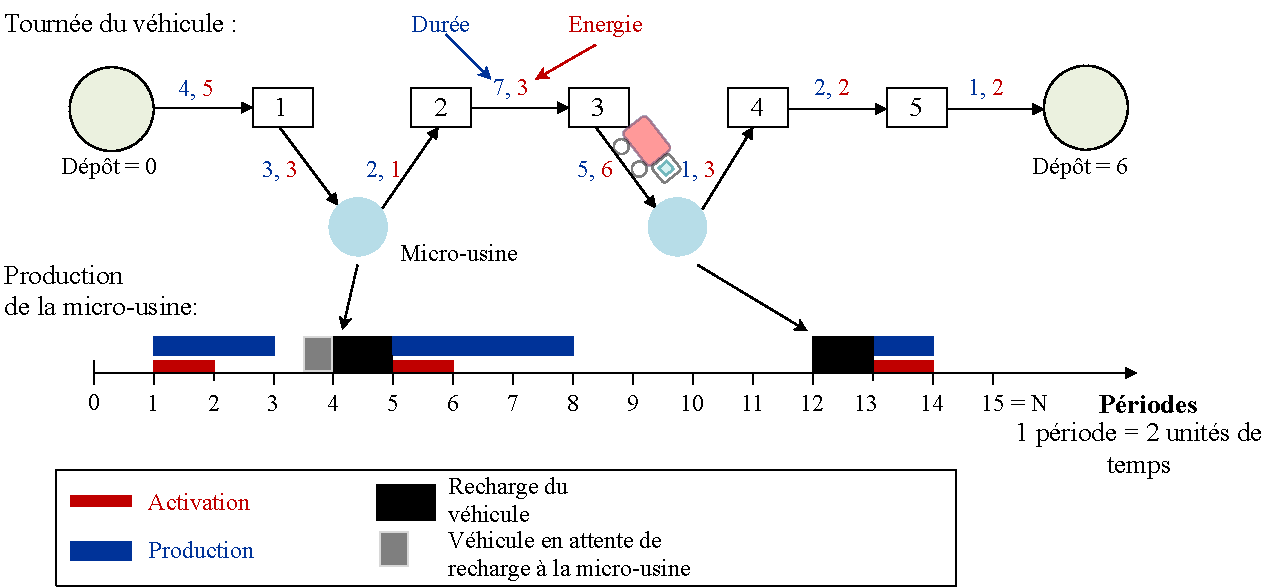
\includegraphics[height=8cm]{images_these/Synchro_exemple.pdf}}
	\caption[Synchonisation du problème VD et du problème PM]{Une solution réalisable correspondant à $p=2$, $E_0=8$, $H_0=4$, $TMax=30$, $Cost^F=7$, $C^{Tank}=15$, $C^{Veh}=15$, $\alpha=1$, ainsi que $t$, $d$, $e$, $\varepsilon$ comme aux figures (\ref{Trip}) et (\ref{exempl_strategie_prod}).}
	\label{Synchro_exemple}
\end{figure}

Le tableau (\ref{Simulation_synchro}) nous donne ensuite l'évolution des couples $(i, j) \in \mathcal{T}$ qui représente le temps au sens de la programmation dynamique, les états $s = (Z, T, V^{Tank}, V^{Veh})$, les décisions $D = (z, x, \delta)$ et les coûts $Cost + \alpha \times T$, induits par cette solution.

\begin{table}[H]
	\centering
	\begin{tabular}{|c|c||c|c|c|c||c||c|c|c|}
		\hline
	\rowcolor{cyan}	\multicolumn{2}{|c||}{temps DPS (i,j)}& \multicolumn{4}{|c||}{Etat $s = (Z, T, V^{Tank}, V^{Veh})$}&Coût $ W$ & \multicolumn{3}{|c|}{Décisions $ D = (z, x, \delta )$ } \\
		\hline
		i & j & Z &T & $V^{Tank}$ & $V^{Veh}$&W=Cost + T & z & x&$\delta$ \\ 
		\hline
		0 & 0 & 0 &0 & 4 & 8&0 + 0 & 0 & 0&0 \\ 
		\hline
		1 &1 & 0 &4 & 4 & 3&0 + 4 & 1 & 0&0 \\ 
		\hline
		2 &1 & 1 &4 & 9 & 3&8 + 4 & 1 & 1&0 \\ 
		\hline
		3 &1 & 1 &4 & 13 & 3&9 + 4 & 0 &0&0 \\ 
		\hline
		4 &1 & 0 &4 & 13 & 3&9 + 4 & 0 & 0&1 \\ 
		\hline
		5 &2 & 0 &12 & 0 & 12&9 + 12 & 1 & 0&0 \\ 
		\hline
		6&	3&	1&	19&	3&	9&	18 + 19&	1&	0&	0\\
		\hline
		7&	3&	1&	19&	8&	9&	20 + 19	&1	&0	&0\\
		\hline
		8&	3&	1&	19&	12&	9&	22 + 19	&0	&0	&0\\
		\hline
		9&	3&	0&	19&	12&	9&	22 + 19&	0&	1&	0\\
		\hline
		10&	3&	0&	19&	12&	9&	22 + 19	&0	&0	&0\\
		\hline
		11&	3&	0&	19&	12&	9&	22 + 19&	0&	0&	0\\
		\hline
		12&	3&	0&	19&	12&	9&	22 + 19&	0&	0&	1\\
		\hline
		13&	4&	0&	27&	0&	12&	22 + 27	&1  &0	&0\\
		\hline
		14&	5&	1&	29&	4&	10&	30 + 29	&0&	0	&0\\
		\hline
		15&	6&	0&	30&	4&	8&	30 + 30	&*&	*	&*\\
		\hline
		
	\end{tabular}
	\caption[Simulation de l'évolution du temps DPS]{Simulation de l'évolution du temps $(i,j)$, $s$, $D$ et $Cost + \alpha \times T$ correspondant à la figure (\ref{Synchro_exemple}). }
	\label{Simulation_synchro}
\end{table}

On a défini l'architecture du \textbf{DPS\_SMEPC}, on présente dans la section suivante l'algorithme général. Pour cela, on définit l'état initial, les caractéristiques d'un état final et le principe de l'algorithme \textbf{DPS\_SMEPC}. 

\subsection{Mise en œuvre algorithmique}

Dans cette partie, on définit l'algorithme général du \textbf{DPS\_SMEPC}, en donnant les données d'entrées, les sorties attendues, les équations de Bellman, et les instructions à exécuter.	

\subsubsection{Equations de Bellman}
Pour tout couple $(i,j)$ qui représente le temps au sens de la programmation dynamique et pour tout état $s=(Z,T,V^{Tank},V^{Veh})$, nous associons la valeur $W$ égale au coût le plus petit possible d'une séquence de transitions réalisables partant de l'état initial $s_0=(0,0,H_0,E_0)$ à la date $(0,0)$ à l'état $s=(Z,T,V^{Tank},V^{Veh})$ à la date $(i,j)$.

Nous concevons l'architecture \textbf{DPS\_SMEPC} selon une stratégie orientée vers l'avenir voir figure (\ref{Ens_etats}) . Pour tout couple $(i, j) \in \mathcal{T}$ qui représente le temps au sens de la programmation dynamique, nous désignons par $S(i, j)$ ce que nous appelons le sous-ensemble d'état lié à $(i, j)$ et qui est en fait un ensemble de triplet $(s, W, Father)$ où W est la valeur définie ci-dessus et $Father$ signifie le couple $((i_f, j_f), s_f)$ où $s_f$ est l'état lié au couple $(i_f, j_f)$ qui nous a permis d'atteindre l'état $s$ au couple $(i, j) \in \mathcal{T}$.
 
\begin{figure}[H]
	\centerline{
		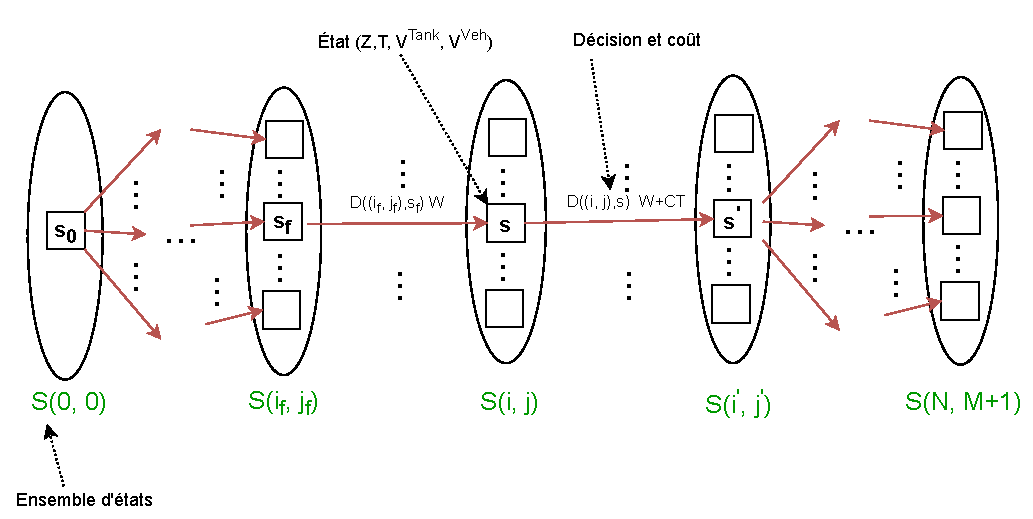
\includegraphics[height=10cm]{images_these/Ens_etats.pdf}}
	\caption[Stratégie de génération des états du DPS\_SMEPC]{La stratégie de génération des états du \textbf{DPS\_SMEPC} est orientée vers l'avenir.}
	\label{Ens_etats}
\end{figure}
Nous analysons le sous-ensemble d'états $S(i, j)$, et pour tout état $s = (Z, T, V^{Tank} , V^{Veh})$, nous générons l'ensemble de décisions possibles $Dec((i, j), s)$. 
Ensuite, pour chaque décision de ce type $D = (z, x, \delta)$, nous générons le couple résultant $(i', j')$, qui représente le temps au sens de la programmation dynamique, et l'état $s' = (Z', T', V'^{Tank} , V'^{Veh})$, ainsi que la valeur $W + CT$, où $CT$ signifie le coût de la transition entre $((i, j), s) \rightarrow ((i', j'), s')$ et $W$ est la valeur associée à $(i, j) \in \mathcal{T}$ et $s$. On a trois scénarios possibles lors de l'ajout de $s'$ dans $S(i',j')$ :
\begin{itemize}[label=$\square$]
	\item Si l'état $s'$ n'apparait pas encore dans l'ensemble d'états $S(i',j')$ alors on l'insère dans $S(i',j')$ avec la valeur $W + CT$ ;
	\item Si l'état $s'$ apparaît déjà dans $S(i', j')$ avec une valeur $W^* > W + CT$, alors $W + CT$ devient la valeur associée à $(i', j')$ et $s'$ ;
	\item Si l'état $s'$ apparaît déjà dans $S(i', j')$ avec une valeur $W^* \leq W + CT$, alors nous rejetons $s'$.
	 
\end{itemize}
\subsubsection{Stratégie d'exploration}
La stratégie d'exploration du temps au sens de la programmation dynamique est la stratégie \textbf{Forward}.
\subsubsection{Algorithme général du DPS\_SMEPC}

La description complète de l'algorithme général du \textbf{DPS\_SMEPC} est résumée à l'algorithme (\ref{algo_DPS_SMEPC}). 

Comme nous le verrons dans la section \ref{regles_de_filtrage}, l'instruction (11) doit être renforcée par des mécanismes de filtrage, qui vont nous permettre de tuer $(s', W', Father')$ au cas où une certaine forme d'in-faisabilité serait prévue, ou au cas où nous pourrions vérifier que le maintien de la tournée définie par $(i', j')$ et $(s', W', Father')$ ne donnera pas une meilleure solution que celle qui existe déjà.

L'instruction (19) nous explique comment nous balayons l'espace-temps, d'une manière qui est cohérente avec son ordre partiel standard. Plusieurs fonctions $Succ_{\Delta}$ peuvent être définie, consistant à balayer $\Delta$ selon les lignes $i$, les colonnes $j$, ou les couches diagonales.

\begin{algorithm} 
	\caption{DPS\_SMEPC}
	\label{algo_DPS_SMEPC}
	\begin{algorithmic}[1]
		\REQUIRE $N$, $M$, $TMax$ $H_0$, $E_0$, $C^{Tank}$, $C^{Veh}$,
		\ENSURE $Current\_Sol$, $Current\_Value$
 		\hline
		\vspace{0.5cm}
		\INITIALISATION
		\STATE $i \leftarrow 0$; $j \leftarrow 0$; $W \leftarrow 0$;
		\STATE $S(0,0) \leftarrow \{(s_0=(0,0,H_0,E_0), W=0, Father=Indéfini)\}$ ;
		\STATE $Current\_Sol \leftarrow Undefined$ ; $Current\_Value \leftarrow +\infty$ ;
		\vspace{0.3cm}
		
		\BOUCLEPRINCIPAL
		\vspace{0.2cm}
		\WHILE{$j+i\leq N+M+1$}
		\FOR{$(s,W,Father)$ dans la liste $S(i,j)$}
		\STATE Générer l'ensemble des décisions possibles $Dec((i,j),s)$ (au sens de la section \ref{liste_decisons});
		\FOR{$D=(z,x,\delta)$ dans $Dec((i,j),s)$}
		\STATE Calculer le couple résultant $(i',j')$ et l'état $s'=(Z',T',V'^{Tank}, V'^{Veh})$, ainsi que le coût de transition $CT$ ; 
		\IF{un triplet $(s', W', Father')$ apparaît déjà dans $S(i', j')$ et si $W' > W + CT$ }
		\STATE Remplacer $(s', W', Father')$ par $(s', W+CT, (s,i,j))$ ;
		\ELSE
		\STATE Insérer $(s', W+CT, (s,i,j))$ dans $S(i',j')$ ;
		\ENDIF
		\IF{$(j'=M+1) \land (T'\leq TMax) \land (V^{Tank}\geq H_0) \land (V^{Veh} \geq E_0) \land (Current\_Value>W+CT)$}
		\STATE $Current\_Value \leftarrow W+CT$ ;
		\STATE $Current\_Sol \leftarrow (s', (s,i,j))$ ;
		\ENDIF
		\ENDFOR
		\ENDFOR
		\STATE $(i, j) \leftarrow Succ_{\Delta}(i,j)$ ;
		\ENDWHILE
	\end{algorithmic}
\end{algorithm}
En utilisant l'algorithme global qu'on vient de présenter, on va donner un schéma d'approximation polynomial du problème \textbf{SMEPC}. 
\section{Un schéma d'approximation polynomial (PTAS) : filtrage par arrondi (Rounding)}
\label{Rounding_filter}

Le \textbf{DPS\_SMEPC} peut être en difficulté dès que $M$ et $N$ sont grands : chaque état est un quadruplet, avec $T$, $V^{Veh}$ et $V^{Tank}$ aux valeurs potentiellement importantes. Néanmoins, nous pouvons remarquer que si nous considérons $TMax$, $C^{Tank}$ et $C^{Veh}$ comme étant limités par des fonctions polynomiales de $N$ et $M$, alors le \textbf{DPS\_SMEPC} devient polynomiale dans le temps puisque le nombre d'états qu'il implique devient également limité par une fonction polynomiale de $N$ et $M$.

En fait, nous pouvons aller plus loin et introduire un schéma d'arrondi du type schéma d'approximation polynomial (PTAS) comme suit : 
\begin{enumerate}
	\item \textbf{Arrondi d'états dans le schéma \textbf{DPS\_SMEPC}} : $L$ étant un nombre entier, alors, pour tout nombre entier $n$ avec comme décomposition binaire $n = a_0 + a_1 \times 2 + \dots + a_q \times 2^q$, nous nous sommes fixés :
	\begin{itemize}[label=$\square$]
		\item Si $q\leq L$ alors $Round(n, L)=n$ alors $Round(n, L)=a_{q-K}\times 2^{q-L}+ \dots + a_q\times 2^q$ ;
		\item Si $q\leq L$ alors $Round^*(n, L)=n$ alors $Round^*(n, L)=a_{q-K}\times 2^{q-L}+ \dots + a_q\times 2^q+2^{q-L}$.
	\end{itemize}
	Deux nombres entiers $n$ et $m$ sont équivalents modulo les $L$ plus grands bits si $Round(n, L) = Round(m, L)$.
	
	Revenons maintenant à notre schéma algorithmique \textbf{DPS\_SMEPC}. Nous supposons tout d'abord que toutes les entrées $d$, $t$, $e$, $\varepsilon$ , $R_i$, $Cost^F$, $Cost^V_i$, $TMax$, $C^{Tank}$ et $C^{Veh}$ de notre modèle \textbf{SMEPC} sont des entiers. $L$ étant un nombre entier, $s_1 = (Z, T_1, V^{Tank}_1, V^{Veh}_1)$ et $s_2 = (Z, T_2, V^{Tank}_2, V^{Veh}_2)$ étant deux états de notre schéma algorithmique \textbf{DPS\_SMEPC}, par extension ils sont équivalents modulo les $L$ plus grands bits si $Round(T_1, L) = Round(T_2, L)$, $Round(V^{Tank}_1, L) = Round(V^{Tank}_2, L)$, $Round(V^{Veh}_1, L) = Round(V^{Veh}_2, L)$.
	
	
	\item \textbf{Le schéma d'approximation \textbf{DPS\_SMEPC}(K)} : 
	
	Soit un certain entier $K\geq 1$, nous transformons l'algorithme (\ref{algo_DPS_SMEPC}) \textbf{DPS\_SMEPC} en un algorithme paramétré \textbf{DPS\_SMEPC}(K) en procédant comme suit :
	\begin{itemize}[label=$\square$]
		\item Nous calculons $L(N, M)$, avec une valeur minimale telle que $2^{L(N,M)}\geq N+M+1$ ; 
		\item Nous étendons la notion d'états, en considérant que tout état $s$ est un quintuplet 
		
		$(Z,\Omega, T,V^{Tank}, V^{Veh})$ associé à un couple $(i,j)$ qui représente le temps au sens de la programmation dynamique, où $\Omega$ nous dit si $T<<i$ ($\Omega=0$), $T==i$ ($\Omega=1$), $(T>>i)\land(T+d_j>p \times i)$ ($\Omega=2$), $(T>>i)\land(T+d_j\leq p \times i)$ ($\Omega=3$) : Cela signifie clairement que nous voulons tenir compte ici du fait (voir la remarque \ref{Remarque_position_veh}) que le positionnement relatif de $T$ et $i$ par les relations $<<$, $>>$ et $==$ agit comme une variable d'état implicite. En raison des effets d'arrondi, qui sont susceptibles de perturber ces relations, nous introduisons une variable , dont le but est d'expliciter les informations fournies par ces positionnements relatifs ; 
		\item Nous faisons en sorte que, à toute itération de la boucle principale de notre algorithme, l'ensemble $S(i, j)$ ne contienne pas deux triplets $(s_1, W_1, Father_1)$ et $(s_2, W_2, Father_2)$ de sorte que respectivement $s_1$ et $s_2$, ainsi que $W_1$ et $W_2$, soient équivalents modulo les $K + 2.L(N, M)$ plus grands bits ; Nous le faisons en donnant la priorité aux triplets $(s_q, W_q, Father_q)$, $q = 1$, $2$, lié à la plus petite valeur de $W_q$ ;
		\item Nous remplaçons les valeurs initiales $H_0$ et $E_0$ par respectivement $Round^*(H_0, K + 1)$ et $Round^*(E_0, K + 1)$ ; 
		\item Nous assouplissons la contrainte de capacité temporelle en remplaçant $TMax$ par 
		
		$Round^*(TMax, K)$ ; De la même manière, nous assouplissons les contraintes de capacité d'hydrogène associées à la fois à la micro-usine et au véhicule en remplaçant les capacités $C^{Tank}$ et $C^{Veh}$ respectivement par $Round^*(C^{Tank}, K)$ et $Round^*(C^{Veh}, K)$ : Cela signifie que $(i, j) \in \mathcal{T}$ étant le couple qui représente le temps au sens de la programmation dynamique actuelle, et $s$ étant l'état actuel, nous calculons l'ensemble de décisions $Dec((i, j), s)$ (instruction 7 ci-dessous) de manière à ce que la faisabilité de toute décision $D = (z, x, \delta)$ soit vérifiée par rapport à la capacité temporelle $Round^*(TMax, K)$ et que les contraintes de capacité d'hydrogène soient vérifiées par rapport aux capacités d'hydrogène $Round^*(C^{Tank}, K)$ et $Round^*(C^{Veh}, K)$. 
	\end{itemize}
\end{enumerate}

\begin{algorithm} 
	\caption{DPS\_SMEPC(K)}
	\label{algo_DPS_SMEPC(K)}
	\begin{algorithmic}[1]
		\REQUIRE $N$, $M$, $TMax$ $H_0$, $E_0$, $C^{Tank}$, $C^{Veh}$, $K$
		\ENSURE $Current\_Sol$, $Current\_Value$
		\hline
		\vspace{0.5cm}
		\INITIALISATION
		\STATE $L \leftarrow L(N,M) $ ; $i \leftarrow 0$; $j \leftarrow 0$; $W \leftarrow 0$; $Current\_Sol \leftarrow Undefined$ ;
		\STATE $Current\_Value \leftarrow +\infty$ ; $S(0,0) \leftarrow \{(s_0=(0,0,H_0,E_0), W=0, Father=Indéfini)\}$ ; 
		\STATE $TMax \leftarrow Round^*(TMax, K)$ ; $C^{Tank} \leftarrow Round^*(C^{Tank}, K)$; 
		\STATE $C^{Veh} \leftarrow Round^*(C^{Veh}, K)$ ; $H_0 \leftarrow Round^*(H_0, K+1)$ ; $E_0 \leftarrow Round^*(E_0, K+1)$ ;
		
		\vspace{0.3cm}
		
		\BOUCLEPRINCIPAL
		\vspace{0.2cm}
		\WHILE{$j+i\leq N+M+1$}
		\FOR{$(s,W,Father)$ dans la liste $S(i,j)$}
		\STATE Générer l'ensemble des décisions possibles $Dec((i,j),s)$ (au sens de la section \ref{liste_decisons}) ;
		\FOR{$D=(z,x,\delta)$ dans $Dec((i,j),s)$}
		\STATE Calculer le couple résultant $(i',j')$ et l'état $s'=(Z', T', V'^{Tank}, V'^{Veh})$, ainsi que le coût de transition $CT$ ; 
		\IF{un triplet $(s'', W'', Father'')$ apparaît déjà dans $S(i', j')$ tel que respectivement $s'$ et $s''$ ainsi que $W+CT$ et $W''$ sont équivalents modulo les $K+L$ plus grand bits et $W+CT<W''$}
		\STATE Remplacer $(s'', W'', Father'')$ par $(s', W+CT, (s,i,j))$ ;
		\ELSE
		\STATE Insérer $(s', W+CT, (s,i,j))$ dans $S(i',j')$ ;
		\ENDIF
		\IF{$(j'=M+1) \land (T'\leq TMax) \land (V^{Tank}\geq H_0) \land (V^{Veh} \geq E_0) \land (Current\_Value>W+CT)$}
		\STATE $Current\_Value \leftarrow W+CT$ ;
		\STATE $Current\_Sol \leftarrow (s', (s,i,j))$ ;
		\ENDIF
		\ENDFOR
		\ENDFOR
		\STATE $(i, j) \leftarrow Succ_{\Delta}(i,j)$ ;
		\ENDWHILE
	\end{algorithmic}
\end{algorithm}
Le DPS-SMPEPC(K) est résumé à l'algorithme (\ref{algo_DPS_SMEPC(K)}).
\begin{theo} (Schéma d'approximation polynomial)
	\label{approx_scheme_pol}
	$K$ étant fixé, le \textbf{DPS\_SMEPC}(K) est polynomial en temps. En outre, pour toute valeur $\varepsilon > 0$, on peut choisir $K$ suffisamment grand de telle sorte que si le \textbf{SMEPC} admet une solution optimale avec la valeur $W^{Opt}$, alors \textbf{DPS\_SMEPC}(K) donne une solution qui est réalisable en ce qui concerne les valeurs initiales $(1 + \varepsilon/ 2)\times H_0$ et $(1 + \varepsilon/ 2)\times E_0$, les valeurs seuils $(1 +\varepsilon )\times C^{Tank}, (1 + \varepsilon)\times C^{Veh}$ et $(1 + \varepsilon)\times TMax$ et dont la valeur de coût $Current\_Value$ n'est pas supérieure à $W^{Opt}+ \varepsilon$.
	\label{FPTAS_theo1} 
\end{theo}
La démonstration de ce théorème se trouve en annexe à la section \ref{approx_scheme_pol_section}.

Malgré le résultat ci-dessus, nous sommes confrontés à un problème qui est l'augmentation du nombre d'états lorsque $N$ et $M$ deviennent de plus en plus grand, et nous devons donc réfléchir à des dispositifs à mettre en place pour diminuer ces états. Dans la section suivante, on présentera quelques mécanismes de filtrage pour résoudre le problème d'explosion d'états.
\section{Mécanismes de filtrage}
\label{regles_de_filtrage}
Les mécanismes de filtrage permettent de diminuer le nombre d'états générés à chaque pas de temps au sens de la programmation dynamique. Si un état ne respecte pas les mécanismes de filtrage alors on le \textbf{tue (i.e. on suppose qu'il n'existe aucune décision possible partant de cet état, l'état n'a donc pas d'état suivant)}. Dans la figure (	\ref{reglesfiltre_impact}), au temps $(i,j)$ au sens de la programmation dynamique, on a 12 états avant l'application des mécanismes de filtrage, une fois les mécanismes de filtrage appliquées, on remarque qu'il reste 6 états. C'est avec ses 6 états qu'on va continuer le processus de prise de décisions.

\begin{figure}[H]
	\centerline{
		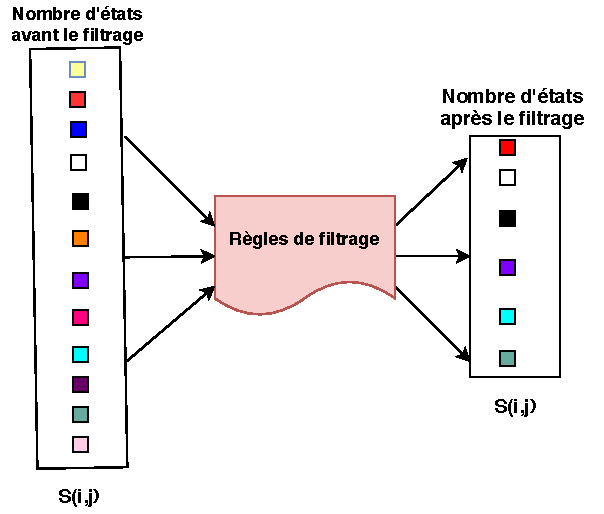
\includegraphics[height=8cm]{images_these/reglesfiltre_impact.pdf}}
	\caption[Impact des mécanismes de filtrage sur le DPS\_SMEPC]{Impact des mécanismes de filtrage sur le \textbf{DPS\_SMEPC} à chaque pas de temps au sens de la programmation dynamique.}
	\label{reglesfiltre_impact}
\end{figure}
%\subsection{Liste des mécanismes de filtrage du \textbf{DPS\_SMEPC}}
Les mécanismes de filtrage nous permettent de diminuer le nombre d'états générés par le \textbf{DPS\_SMEPC}. Dans cette partie, on conçoit trois grands types de mécanismes de filtrage : les mécanismes de filtrage par relations de dominance, les mécanismes de filtrage logique et les mécanismes de filtrage basées sur la borne supérieure/inférieure. Les mécanismes de filtrage par relations de dominance consiste à se débarrasser de tous les états dominés. Les mécanismes de filtrage logique sont basées sur l'anticipation des incohérences. Plus précisément, il s'agit de supprimer tous les états qui nous « conduirons » à des solutions non réalisables. Les mécanismes de filtrage basées sur la borne supérieure/inférieure consistent à supprimer tous les états qui nous « conduirons » à des solutions moins bonnes qu'une solution connue qui a été calculée avec une heuristique rapide.

\subsection{Mécanismes de filtrage par relations de dominance }
Les mécanismes de filtrage par relations de dominance consistent à supprimer des états qui sont dominés par d'autres états qui existent. Il existe deux types de mécanismes de filtrage par relations de dominance : les mécanismes de filtrage par relations de dominance forte et les mécanismes de filtrage par relations de dominance faible. Soit $(i,j)$ un couple qui représente le temps au sens de la programmation dynamique du \textbf{DPS\_SMEPC}. Si les deux états $s_1=(Z_1,T_1,V_1^{Tank},V_1)^{Veh}$ et $s_2=(Z_2,T_2,V_2^{Tank},V_2)^{Veh}$ donné respectivement avec les valeurs $W_1$ et $W_2$ et appartenant à $(i,j)$ sont tels que : $W_1\leq W2$, $T_1\leq T_2$, $Z_1\geq Z_2$, $V^{Tank}_1\geq V^{Tank}_2$, $V^{Veh}_1\geq V^{Veh}_2$ alors $s_1$ domine $s_2$, et nous tuons l'état $s_2$ (i.e. nous le retirons de la liste des états associés à $(i, j)$). Ce mécanisme de filtrage par relations de dominance forte a peu de pouvoir de filtrage, car elle est trop restrictive. 

Néanmoins, d'autres mécanismes de filtrage par relation de dominance peuvent être mis en œuvre, par exemple le mécanisme de filtrage par relations de dominance faible heuristique. L'idée ici est de concevoir un mécanisme de filtrage flexible qui nous aidera à maintenir le nombre d'états sous un certain seuil noté $NS$. Soit $A$, $B$, $C$, $D$, $E$ des paramètres positifs. Nous procédons de manière à ce que pour tout couple de temps $(i, j)$, nous ne gardions que les $NS$ états ayant le plus petit : $A\times W + B\times T - C\times Z - D\times V^{Tank} - E\times V^{Veh}$ . Le choix des valeurs $ (A, B, C, D, E)$ est un problème en soi. On peut par exemple considérer les valeurs de conversion suivantes : 
$(A, B, C, D, E) = (1, , Cost^F, Cost^V, Cost^V)$, où $Cost^V$ est la moyenne de $Cost^V_i, i= 0, \dots, N-1$, valeurs.



\subsection{Mécanismes de filtrage logique} 
\label{Logique_SMEPC_ALGO}
Les mécanismes de filtrage logique tuent des états si ceux-ci ne respectent pas certains mécanismes logiques. Par exemple, s'il ne reste pas assez de temps ou d'énergie pour que le véhicule puisse finir sa tournée.

Considérons l'état $s=(Z,T,V^{Tank}, V^{Veh})$ appartenant au temps $(i,j)$ au sens de la programmation dynamique, l'idée est d'anticiper l'in-faisabilité d'une tournée à partir des états $s$ appartenant au temps $(i, j)$. Cette in-faisabilité peut être liée soit à un manque de temps (impossible de réaliser la tournée du véhicule avant l'échéance $TMax$), soit à la production d'énergie (impossible d'obtenir suffisamment d'hydrogène pour réaliser la tournée). Plus précisément, pour tout $j = 0, \dots, M$, nous obtenons une estimation approximative de l'énergie et du temps nécessaires pour permettre au véhicule d'aller de la station $j$ au dépôt final en procédant comme suit : 

\begin{itemize}[label=$\square$]
	\item Nous désignons par $\Omega_0, \dots, \Omega_{M-j}$ les quantités $(\varepsilon_k + \varepsilon_{k+1}^* - e_k)$, $j \leq k \leq M$, ordonnées par ordre croissant  $\Omega_0 < \dots < \Omega_{M-j}$;
	\item Nous désignons par $\Delta_0, \dots, \Delta_{M-j}$ les quantités $(d_k + d_{k+1}^* - t_k)$, $j \leq k \leq M$, ordonnées par ordre croissant. Pour toute station $j$

	\item Nous désignons par $Prod\_Max(i)$ la quantité $\sum_{k\geq i}R_k$ : la micro-usine ne peut produire plus de $Prod\_Max(i)$ quantité d'hydrogène à partir de la période $p\times i$ ;
	\item Pour calculer $H_j$, $j=\{0, \dots M\}$ l'énergie nécessaire au véhicule pour aller de la station $j$ au dépôt final on exécute l'algorithme (\ref{algo_estimation_energie}) nommé \textbf{Estimation-énergie(j)}. Le véhicule devra recharger au moins $H_j - V^{Veh}$ afin de réaliser sa tournée à partir de $j$ et effectuer au moins $Refuel$ opérations de recharge en hydrogène. Pour calculer $Refuel_j$, $j=\{0, \dots M\}$ le nombre de recharge nécessaire au véhicule pour aller de la station $j$ au dépôt final on exécute l'algorithme (\ref{algo_estimation_energie}) nommé \textbf{Estimation-énergie(j)}.
	\item En tenant compte du nombre de recharge $Refuel_j$, une borne inférieure noté $\Phi_j =\sum_{k\geq j}t_k + \sum_{q=0, \dots, Refuel_j-1}\Delta_q$ sur le temps qu'il faut au véhicule pour aller de $j$ au dépôt final peut être déduite. Le véhicule a donc besoin d'au moins $\Phi_j$ unités de temps pour effectuer sa tournée de $j$ au dépôt final ;
	\begin{algorithm} 
		\caption{Estimation-énergie(j)}
		\label{algo_estimation_energie}
		\begin{algorithmic}[1]
			\REQUIRE $e$,$E_0$ $\Omega$, $C^{Veh}$, $j$
			\ENSURE $H$, $Refuel$
			\hline
			\vspace{0.5cm}
			\INITIALISATION
			\STATE $H \leftarrow E_0+\sum_{k\geq j} e_j  $; 
			\STATE $Not Stop$;
			\STATE $Refuel \leftarrow 0$;
			
			\vspace{0.3cm}
			
			\BOUCLEPRINCIPAL
			\vspace{0.2cm}
			\WHILE{$Not Stop$}
			\STATE $Refuel\_Aux \leftarrow \lfloor H/C^{Veh} \rfloor$
			\IF{$Refuel\_Aux=Refuel$}
			\STATE  $Stop$;
			\ELSE
			\STATE $H \leftarrow H+\sum_{q=Refuel, \dots, Refuel\_Aux} \Omega_q$;
			\STATE $Refuel \leftarrow Refuel\_Aux$ ;
			\ENDIF
			\ENDWHILE
		\end{algorithmic}
	\end{algorithm}
\end{itemize}

Cela nous permet d'énoncer les mécanismes de filtrage logique suivantes : 
\begin{enumerate}
	\item Le mécanisme de filtrage basée sur le temps est le suivante si $( \Phi_j \geq TMax - T + 1)$, alors on tue l'état $s = (Z, T, V^{Tank} , V^{Veh})$ lié au temps $(i, j)$, au sens de la programmation dynamique, car il ne reste pas suffisamment de temps au véhicule pour finir sa tournée ;
	
	\item Le mécanisme de filtrage basée sur l'énergie est énoncée comme suit si $H_j > V^{Veh} + Prod\_Max(i) + V^{Tank}$, alors on tue l'état $ s = (Z, T, V^{Tank}, V^{Veh})$ lié au temps $(i, j)$, au sens de la programmation dynamique, car il n'y aura pas suffisamment d'énergie pour que le véhicule puisse finir sa tournée.
\end{enumerate}
Si nous nous référons à la description de l'algorithme  (\ref{algo_DPS_SMEPC}) nommé \textbf{DPS\_SMEPC}, nous voyons que l'instruction 12 doit ensuite être transformé en l'instruction suivante :
appliquer successivement à $s'$ le mécanisme de filtrage par relation de dominance forte, le mécanisme de filtrage basée sur le temps et le mécanisme de filtrage basée sur l'énergie ;
Si $s'$ n'a pas été tué alors insérer $(s', W + CT, (s, W, Father))$ dans $S(i', j') $.


\subsection{Mécanismes de filtrage par estimation optimiste}
\label{CostMin_chap5}
Nous définissons, pour toute quantité d'énergie $V$ et toute période $i$, le coût minimal de production $CostMin_{i, V, Z}$ requis pour produire $V$ unités d'hydrogène entre la date $p\times i$ et la date $TMax$, $Z$ désignant l'état de la micro-usine à la fin de la période $i - 1$ : si $V = 0$ alors $CostMin_{N, V, Z} = 0 $, sinon, $CostMin_{N, V, Z}$ n'est pas défini et, $CostMin_{i, V, Z} = Inf [CostMin_{i + 1, V, 0}, CostMin_{i + 1, V - R_i, 1} + (Cost^F.(1 - Z) + Cost^V_i)]$. 

Nous calculons $CostMin$ au moyen d'un DPS backward, et gardons en mémoire les valeurs $CostMin_{i, V, Z}$, à condition que la portée des valeurs de $V$ ne soit pas trop grande (sinon nous effectuons un certain arrondissement des valeurs de $V$).

Si l'on donne maintenant une paire de temps $(i, j)$ et un état connexe $s = (Z, T, V^{Tank}, V^{Veh})$ avec la valeur $W$. On obtient alors une borne supérieure/inférieure $LB$ de la meilleure valeur \textbf{SMEPC} qui peut être dérivée de $(i, j)$ et $s$ : $LB((i, j), s) = \alpha \times \Phi_j+ CostMin(i, (H_j - V^{Tank})^+, Z)$.

Si nous supposons maintenant que nous disposons d'une valeur réalisable $Current\_Value$ de \textbf{SMEPC} réalisable, alors nous pouvons mettre en œuvre le mécanisme de filtrage suivante : 

\textbf{ le filtrage basée sur la borne supérieure/inférieure est si $W+LB((i,j),s)\geq Current\_Value$ }, alors on tue l'état $s = (Z, T, V^{Tank}, V^{Veh})$ associé au temps $(i,j)$.

Si nous nous référons à la description de l'algorithme \textbf{DPS\_SMEPC} (\ref{algo_DPS_SMEPC}), nous voyons que l'instruction 12 doit ensuite être transformé en l'instruction suivante :
appliquer successivement à $s'$ le mécanisme de filtrage par relation de dominance forte, le mécanisme de filtrage basée sur le temps et le mécanisme de filtrage basée sur l'énergie ;
Si $s'$ n'a pas été tué alors appliquer à $s'$ le mécanisme de filtrage basée sur la borne supérieure/inférieure;
Si $s'$ n'a pas été tué alors insérer $(s', W + CT, (s, W, Father))$ dans $S(i', j') $.

Dans cette partie,on a défini les mécanismes de filtrage basées sur la borne supérieure/inférieure. Partant d'un état $ s = (Z, T, V^{Tank}, V^{Veh})$ lié au temps $(i, j)$ et dont la valeur est $W$, on a estimé le coût minimal (constitué du coût de production $CostMin_{i,V^{Veh}, Z}$ et de la longueur de la tournée $\Phi_j$ ) qu'il faut au véhicule pour aller de la station $j$ au dépôt final. Si la valeur $W + CostMin_{i,(H_j - V^{Tank})^+, Z} + \alpha \times \Phi_j$ est plus grande que le coût d'une solution connue $Current\_Value$ (pré-calculée par exemple avec une heuristique) alors on tue l'état $s$.% d'une solution contenant $s$. Puisqu'une solution est un chemin dont les nœuds sont des états et les arcs sont des décisions.

Plus précisément, on va présenté par la suite comment est calculé $CostMin(i, V, Z)$ à l'aide d'un algorithme qu'on nommera « Cout minimal production ». Pour cela on présentera le principe, les données d'entrées, les sorties et le pseudo-code de l'algorithme « Cout minimal production ».

%\textbf{Nous expliquons ici comment est calculé $CostMin$ qui représente le coût minimal de production d'une quantité $P$ d'hydrogène à partir d'un état de la micro-usine $(Z,t)$}


\textit{ \textbf{Principe de « Cout minimal production »}}

On calcule le coût minimal de production d'au moins $V$ unités d'hydrogène
entre l'instant $p\times i$ et l'instant $TMax$ à l'aide d'un programme dynamique qui fonctionne en backward. On suppose que l'état de la micro-usine pendant la période $i-1$ est $Z$.
On initialise $CostMin_{N,Z,0}$ à $ 0$ car le coût de production de 0 unité d'hydrogène est nul, et $CostMin_{N,Z,V}$ est initialisée à $+\infty$.

A l'instant $p\times i$ on a deux cas possibles :
\begin{enumerate}
	\item \textbf{On produit durant la période $i$ la quantité $R_{i}$ d'hydrogène}, il reste la quantité $V-R_{i}$ à produire à partir de la période $i+1$. Pour calculer le coût de production, nous avons deux possibilités :
	\begin{itemize}[label=$\square$]
		\item Il faut démarrer la micro-usine c'est-à-dire que la micro-usine ne produisait pas pendant la période $i-1$ $(Z=0)$ et on décide de produire pendant la période $i$. Le coût de production durant la période $i$ est donc $Cost^v_i+Cost^F$. Il reste à calculer le coût minimal de production d'au moins $V-R_{i}$ à partir de la période $i+1$ sachant que la machine de production produit durant la période $i$ ;
		
		\item La micro-usine est déjà en marche pendant la période $i-1$ $(Z=1)$ et on décide de produire durant la période $ i$. Le coût de production durant la période $i$ est donc $Cost^v_i$. Il reste à calculer le coût minimal de production d'au moins $V-R_{i}$ à partir de la période $i+1$ sachant que la machine de produit durant la période $i$.
	\end{itemize}
	\item \textbf{On ne produit pas durant la période $i$} donc je dois produire au moins la quantité $V$ à partir de $i+1$. Le coût de production durant la période $i$ est 0. Il reste à calculer le coût minimal de production d'au moins $V$ à partir de la période $i+1$ sachant que la machine de production ne produit pas durant la période $i$.
\end{enumerate}
Ici, on veut calculer, une valeur $CostMin_{i,Z,V}$, qui, pour tout $i=0, \dots, N$, va nous donner la valeur du coût minimal d'une production d'au moins $V$, $V=0, \dots, PMAX$, dès lors que l'on démarre à la période $i$, avec la micro-usine en état $Z=\{0,1\}$. On ne tient pas compte de la capacité de la citerne. La période $-1$ est une période fictive qui correspond à l'état initial de la machine de production. $PMAX$ est fourni :
\begin{itemize}[label=$\square$]
	\item Soit comme associé à une tournée pré-calculée, $PMAX$ est alors la quantité $\sum_{q=1}^{Q}u_q-E_0$. $Q$ est le nombre de recharge et $u_q$ la quantité chargée pendant la $q^{ieme}$  recharge ;
	\item Soit comme estimée indépendamment de cette tournée, $PMAX$ est alors $2 \times \sum_{j=0}^{M}e_j $.
\end{itemize} 

\textit{ \textbf{Entrées / Sorties de « Cout minimal production »}}

Les entrées sont :
\begin{itemize}[label=$\square$]
	\item $N$,$Cost^F$, $R_i$, $Cost^V_i$ ;
	\item $PMAX \sim$ la quantité maximale à produire avant la période $N$ ;
	\item $\bar{\bar{q}}_i \sim $ la quantité maximum d'hydrogène qu'on peut produire entre les périodes $i$ et $N-1$ incluses. $\bar{\bar{q}}_i=\sum_{k\geq i}R_k$.
	
\end{itemize}

La sortie est :

\begin{itemize}[label=$\square$]
	\item $ CostMin_{i,Z,V} \sim$ la valeur du coût minimal d'une production $V$, $V=0, \dots, PMAX$, dès lors que l'on démarre la production à la période $i$, $Z$ est l'état de la micro-usine à la fin de la période $i-1$.
	
	$Z_{-1} = 0$ qui signifie que l'usine est à l'arrêt sur la période fictive $-1$.
\end{itemize}

\textit{ \textbf{Algorithme « Cout minimal production »}}

Pour calculer les valeurs du vecteur $CostMin_{i,Z,V}$ on procède en backward, on commence à la période $N-1$. Dans l'algorithme (\ref{ree1}), nous commençons par remplir les cases $i=N$ car on connait qu'à la fin du processus soit on a atteint la production demandée et on ne produit plus, soit on ne peut pas produire en $N$ périodes la quantité demandée. 
\textbf{$CostMin_{i,Z,V}$ réponds à la question comment produire au moins $V$ unités d'hydrogène au coût le plus faible à partir de la période $i$.}


\begin{algorithm} 
	\caption{Cout minimal production}
	\label{ree1}
	\begin{algorithmic}[1]
		\REQUIRE $N$, $PMAX$, $R$, $\bar{\bar{q}}$, $Cost^F$, $Cost^V$,
		\ENSURE $CostMin$
		\hline
		\vspace{0.5cm} 
		\INITIALISATION
		\FOR{$Z=0$ \TO $1$}
		\STATE $CostMin_{N,Z,0}  \leftarrow 0$; /* \textbf{Produire 0 coûte 0} */ 
		\FOR{$V=1$ \TO $PMAX$}
		\STATE $CostMin_{N,Z,V}  \leftarrow  +\infty$;
		\ENDFOR
		\ENDFOR
		
		\vspace{0.3cm}
		
		\BOUCLEPRINCIPAL
		\vspace{0.2cm}
		\FOR{$i=(N-1)$ \TO $0$}
		\FOR{$Z=0$ \TO $1$}
		\FOR{$V= 1$\TO $PMAX$}
		\IF{($V > \bar{\bar{q}}_i$)}
		\STATE $CostMin_{i,Z,V}  \leftarrow +\infty$; /* \textbf{Impossible de produire V en commençant à la période $i$} */
		\ELSE
		\STATE $P1 \leftarrow Sup(V-R_i,0)$; /* \textbf{La micro-usine produis} */
		%	\STATE $E1 \leftarrow 1$;
		\STATE $C1 \leftarrow Cost^v_i+(1-Z)\times Cost^F$; 
		\STATE  $CostMin_{i,Z,V}  \leftarrow Inf(C1+CostMin_{i+1,1,P1}, CostMin_{i+1,0,V})$; /* \textbf{$CostMin_{i+1,0,V}$ correspond à je ne produis pas} */
		/* \textbf{$CostMin_{i,Z,V}$ est le coût minimum de production si on produit à partir de la période i.} */
		\ENDIF
		\ENDFOR
		\ENDFOR
		\ENDFOR
	\end{algorithmic}
\end{algorithm}


On a présenté les mécanismes de filtrage qui permettent de diminuer le nombre d'états générés par le \textbf{DPS\_SMEPC}. Le mécanisme de filtrage basée sur la borne supérieure/inférieure a besoin de la valeur d'une solution connue du problème \textbf{SMEPC}. On va calculer cette solution à l'aide d'une heuristique qui sera présentée à la section suivante. Cette heuristique est une adaptation gloutonne du \textbf{DPS\_SMEPC}


\subsubsection{Borne supérieure calculée par une adaptation gloutonne du DPS\_SMEPC}

On désignera par Greedy-SMEPC l'algorithme de calcule d'une borne supérieure par une heuristique qui est une adaptation gloutonne du \textbf{DPS\_SMEPC}.
La transformation du \textbf{DPS\_SMEPC} en un algorithme glouton afin d'obtenir une borne supérieure $W^{Curr}$ peut être réalisée en utilisant notre schéma de programmation dynamique et en effectuant un parcours en avant dans le réseau d'états du \textbf{SMEPC}, en choisissant à chaque pas de temps au sens de la programmation dynamique l'état qui à la meilleur valeur $LB$ (décrite à la section précédente). On continuera le processus de prise de décision unique ment avec l'état sélectionné.

Néanmoins, nous devons veiller à éviter les stratégies qui verraient à la fois la micro-usine attendre de meilleurs prix $Cost^V_i$, de meilleures rendement de production $R_i$, et le véhicule attendre à la micro-usine pour une meilleure opportunité de chargement. Comme notre capacité à anticiper les incohérences liées à un manque de temps ou à un manque de capacité de recharge en hydrogène ne découle que de dispositifs d'approximation, il existe un risque que de telles stratégies d'attente fassent échouer notre processus de calcul d'une solution possible. Donc, afin de faire diminuer ce risque de défaillance, nous interdisons :
\begin{itemize}[label=$\square$]
	\item Les décisions $(z = 0, x = 1)$ liées à des situations où T == i et où le réservoir de la micro-usine n'est pas suffisamment chargé pour permettre de faire le plein du véhicule ; 
	\item Les décisions $(z = 0, x = 0)$ liées à des situations où $T << i$ et $(p.i - T) \leq d_j$, et où le réservoir de la micro-usine n'est pas suffisamment chargé pour permettre de faire le plein du véhicule ; 
	\item Décisions $(z = 0, x = 0, \delta= 0)$ liées à des situations où $T << i$ et $(p.i - T) \geq d_j$, le véhicule décide de continuer sa tournée sans produire.
\end{itemize}
L'algorithme Greedy-SMEPC est décrit à l'algorithme (\ref{Greedy-SMEPC}). L'instruction 6 est exécutée telle que :
\begin{itemize}[label=$\square$]
	\item La décision $(z, x, \delta)$ n'est pas interdite selon les mécanismes d'interdiction ci-dessus ;
	\item L'état résultant $s_1 = (Z_1, T_1, V^{Tank}_1,V^{Veh}_1)$ n'est pas tué au temps résultant $(i_1, j_1)$ par les mécanismes de filtrage logique ci-dessus ;
	\item $W + Transition\_Cost + LB((i_1, j_1), s_1)$ est le plus petit possible, où $Transition\_Cost$ signifie le coût de la transition induite par l'application de $(z, x, \delta)$ à $s$ au temps $(i, j)$ au sens de la programmation dynamique.
\end{itemize}

\begin{algorithm} 
	\caption{Greedy\_SMEPC}
	\label{Greedy-SMEPC}
	\begin{algorithmic}[1]
		\REQUIRE $N$, $M$, $TMax$ $H_0$, $E_0$, $C^{Tank}$, $C^{Veh}$,
		\ENSURE $Sol\_Greedy$, $Val\_Greedy$
		\hline
		\vspace{0.5cm}
		\INITIALISATION
		\STATE $i \leftarrow 0$; $j \leftarrow 0$; $W \leftarrow 0$; $Not stop$ ;
		\STATE $S(0,0) \leftarrow \{(s_0=(0,0,H_0,E_0), W=0, Father=Indéfini)\}$ ;
		\STATE $Sol\_Greedy \leftarrow Undefined$ ; $Val\_Greedy \leftarrow +\infty$ ;
		\vspace{0.3cm}
		
		\BOUCLEPRINCIPAL
		\vspace{0.2cm}
		\WHILE{$Not stop$}
		\STATE Définissez l'état actuel $s = (Z, T, V^{Tank} , V^{Veh})$, la valeur correspondante = $W$ et la paire de temps actuelle = $(i, j)$ ;
		\STATE Prenez une décision réalisable (au sens de la section \ref{liste_decisons}) $(z, x, \delta)$ ;
		\IF{$(z, x, \delta)$ n'existe pas}
		\STATE Stop ; /* \textbf{Echec : l'algorithme n'a pas trouvé de solution} */
		\STATE $Sol\_Greedy \leftarrow Undefined$ ; $Val\_Greedy \leftarrow +\infty$ ;
		\ELSE
		\IF{$j_1=M+1$}
		\STATE Stop ; /* \textbf{Succès : l'algorithme a trouvé une solution} */
		\STATE $Val\_Greedy = W+Transition\_Cost$ ;
		\STATE$Sol\_Greedy=(s_1, (s,i,j))$ ;
		\ELSE
		\STATE Exécuter la décision $(z,x,\delta)$ : mettre à jour i,j,s et la valeur $W$ associée ;
		\ENDIF
		\ENDIF
		\ENDWHILE
	\end{algorithmic}
\end{algorithm}

Dans l'heuristique décrite par l'algorithme (\ref{Greedy-SMEPC}), on sélectionne à chaque pas de temps au sens de la programmation dynamique un unique état pour continuer le processus de prise de décisions. Lors de la phase expérimentation de cet algorithme,on a remarqué qu'on avec beaucoup de cas d'échec c'est-à-dire qu'on obtient aucune solution pour une grande partie des instances. On peut alors au lieu de sélectionner un seul état, sélectionner $NS > 1$ états ayant les meilleures valeurs $LB$ pour continuer le processus de prise de décisions, cette procédure sera appelée \textbf{Greedy-SMEPC}(NS). Ou alors, on peut sélectionner $NS > 1$ états ayant les meilleures valeurs $LB$ et $BS > 1$ états ayant les pires valeurs $LB$ pour continuer le processus de prise de décisions.

\subsection{Mécanismes de filtrage heuristique}
Notre objectif dans cette section est de décrire des mécanismes de filtrage heuristique qui serviront à diminuer le nombre d'états de l'algorithme général du \textbf{DPS\_SMEPC} quitte à induire un certain niveau d'approximation.
On rappelle qu'un état d'un temps $(i,j)$ est défini par un quadruplet $ (Z, T, V^{Tank}, V^{Veh})$, avec :

\begin{itemize}[label=$\square$]
	\item $Z$ : l'état de la micro-usine de production d'hydrogène ;
	$$
	Z= \left\{
	\begin{array}{ll}
	1 & \mbox{si la micro-usine est active à la fin de la période $i-1$.} \\
	0 & \mbox{sinon.}
	\end{array}
	\right.
	$$
	\item $V^{Tank} $ : la quantité d'hydrogène dans la citerne à la micro-usine au début de la période $i$ ;
	
	\item $V^{Veh} $ : la quantité d'hydrogène dans le réservoir du véhicule lorsqu'il arrive à la station $j$ ;
	
	\item $T \in 0, \dots, TMax$ est une date signifiant :
	\begin{itemize}
		\item Si $T >> i$ alors le véhicule est en route vers la station $j$ et il y arrivera à la date $T$ (Voir figure (\ref{positions_vehicule})) ;
		\item Si $T<<i$ alors le véhicule est entre la station $j$ et la micro-usine. Le véhicule peut être entrain d'attendre à la micro-usine pour être rechargé (Voir figure (\ref{positions_vehicule})) ;
		\item Si $T==i$ alors le véhicule se trouve à la station $j$, et doit choisir entre aller à la station $j+1$ ou aller à la micro-usine se recharger (Voir figure (\ref{positions_vehicule})).
	\end{itemize}
\end{itemize}

On fixe un paramètre entier $K$ dit de fluidification (on pourra utiliser par exemple $K=10$ ou $K=5$). Pour chaque station $j$, on pose :
\begin{itemize}[label=$\square$]
\item $\Delta_j = \sum_{ 0 \leq s \leq j-1} d_s$
\item $\Delta^*_j = TMax - \sum_{ j \leq s \leq M}d_s$
\item $\Pi_j=\Delta^*_j-\Delta_j$.
\end{itemize}
Lorsqu'on est à une paire de temps $(i_0,j_0)$ et que l'on vient de générer, à partir d'un état $E_0$
 et d'une décision $D$ un nouvel état $E=(Z, T, V^{Tank}, V^{Veh})$ accompagné d'une valeur $W$ et associé au temps $(i,j)$ alors :
 \begin{enumerate}
 	\item On applique tous les mécanismes de filtrage décrit précédemment ;
 	\item Si l'état $E$ n'a pas été supprimé par ces mécanismes de filtrage alors on balaie l'ensemble des états du temps $(i,j)$ et chaque fois que l'on rencontre un état $E_1=(Z_1, T_1, V^{Tank}_1, V^{Veh}_1)$ accompagné d'une valeur $W_1$, on procède comme suit :
 	
 	Si $Z =Z_1$ et $|V^{Tank} - V^{Tank}_1| \leq (C^{Tank} / K)$ et $|V^{Veh} - V^{Veh}_1| \leq (C^{Veh} / K)$ et $|T - T_1| \leq (\Pi_j / K)$ alors on dit que $E$ et $E_1$ sont équivalents modulo $K$ :
 	\begin{itemize}[label=$\square$]
 		\item si $W<W_1$ alors on remplace $E_1$, $W_1$ par $E$, $W$ dans les états du temps $(i,j)$ ;
 		\item dans le cas inverse, on ne fait rien, donc on n'insère pas $E$, $W$ parmi les états du temps $(i,j)$ ;
 	\end{itemize}
 
 \end{enumerate}
 

On vient de présenter l'algorithme général du \textbf{DPS\_SMEPC}, les mécanismes de filtrage de cet algorithme et un algorithme qui calcule une borne supérieure pour le \textbf{DPS\_SMEPC}. Dans la section suivante, on va mesurer l'impact des mécanismes de filtrage sur le nombre d'états générés par le schéma de programmation dynamique \textbf{DPS\_SMEPC} qui résout le problème \textbf{SMEPC} et l'efficacité de l'algorithme Greedy-DPS par rapport à l'algorithme \textbf{DPS\_SMEPC}.


\section{Description d'une heuristique rapide $He$ pour résoudre SMEPC}
\label{Heuristique_rapide}
Dans cette section, on va décrire une heuristique rapide nommée $He$ qui calcule une solution d'une instance du problème SMEPC très rapidement.
Nous proposons ici une nouvelle modélisation du problème du véhicule dans laquelle la micro-usine nommée nœud 0 est distincte du dépôt nommé nœud $D$. Nous avons 3 types d'arc mais leur signification est totalement définie par leur origine. Un arc dont l'origine est $j$, $j=0, \dots, M$ signifie que "le véhicule fait le plein de carburant après la station $j$" (le véhicule fait le plein après le dépôt dans le cas $j=0$).
Dans les sous-sections suivantes, nous expliquons comment le problème VD peut être modélisé par un graphe orienté.
\subsection{Le graphe}
Le problème \textbf{VD} peut être modélisé en un problème de plus court chemin dans un graphe $G$.
Si on suppose que le véhicule fait le plein à chaque recharge, VD peut être modélisé sous forme d'un graphe orienté $G = (V,E)$ qui se construit de la façon suivante :

Son ensemble $V$ de sommets est l'ensemble $\{D,0,1, \dots, M, M+1\}$. $D$ et $M+1$ représentent respectivement le dépôt au début et à la fin du trajet du véhicule. Un noeud $j$, $j=0, \dots, M$ correspond au fait que le véhicule se trouve à la micro-usine après avoir quitté la station $j$, ou juste après avoir quitté le dépôt si $j=0$.

Dans $E$, il existe trois types d'arcs :

\begin{itemize}[label=$\square$]
	
	\item \textbf{Arcs de type} 1 : Un arc $(j,j' ) \in E$, $0\leq j<j'\leq M$, indique que le véhicule est capable de se rendre de la micro-usine (après la station $j$) à la micro-usine (après la station $j'$) sans opération de recharge. Cet arc existe si l'inéquation (\ref{arcs_1}) est vérifiée. Cette inéquation signifie que la quantité d'énergie dont a besoin le véhicule pour réaliser ce trajet, ne doit pas être supérieure à la capacité maximale du véhicule.
	
	\begin{equation}\label{arcs_1}
	\begin{align}
	\varepsilon^*_{j+1}+\sum_{j+1 \leq k \leq j'-1} e_k + \varepsilon_{j'} \leq C^{Veh}&  & \forall j < j'= 0, \dots, M
	\end{align}
	\end{equation}
	
	\item \textbf{Arcs de type} 2 : Un arc $(D,j)\in E$, $0 \leq j \leq M$, signifie que :
	\begin{itemize}
		\item le véhicule peut aller du dépôt à la micro-usine juste après le dépôt (si $j=0$) ;
		\item le véhicule peut aller du dépôt à la station $j$ sans faire le plein (si $j\geq1$).
	\end{itemize}
	L'énergie initiale $E_0$ doit être suffisante pour effectuer ce trajet. Par conséquent, cet arc existe si l'inéquation (\ref{arcs_2}) est vérifiée.
	
	\begin{equation}\label{arcs_2}
	\begin{align}
	\sum_{k=0, \dots, j-1} e_k + \varepsilon_{j} \leq E_0&  & \forall j = 0, \dots, M
	\end{align}
	\end{equation}
	
	\item \textbf{Arcs de type} 3 : Les arcs $(j,M+1) \in E$, $0 \leq j\leq M$ signifient que le véhicule peut aller de la micro-usine après la station $j$, jusqu'au dépôt final sans faire le plein. De plus, le véhicule doit arriver au dépôt avec au moins son énergie initiale $E_0$. Cet arc existe si l'inéquation (\ref{arcs_3}) est vérifiée.
	
	\begin{equation}\label{arcs_3}
	\begin{align}
	\varepsilon^*_{j+1}+\sum_{k=j+1, \dots, M} e_k + E_0\leq C^{Veh}&  & \forall j = 0, \dots, M
	\end{align}
	\end{equation}
	
\end{itemize}

\subsection{Les poids sur les arcs}
Soit $P=(D, j_1, \dots, j_q, M+1)$ un chemin entre $D$ et $M+1$ dans $G$. La longueur de $P$ est égale à :

$\sum_{k=0, \dots, j_1-1} t_k +d_{j_1} + d^*_{j_1+1}+p+ \sum_{k=j_1+1 \dots j_2-1} t_k +d_{j_2} +d^*_{j_2+1}+p+ \dots+ \sum_{k=j_{q-1}+1, \dots, j_q-1}t_k + d_{j_q} +d^*_{j_q+1}+p+ \sum_{k=j_q+1, \dots, M}t_k = \sum_{k=0, \dots, M} t_k + d_{j_1}+d^*_{j_1+1}+p-t_{j_1}+d_{j_2}+d^*_{j_2+1}+p-t_{j_2}+ \dots +d_{j_q}+d^*_{j_q+1}+p-t_{j_q}$

Nous désignons par $detour(j)$ la distance supplémentaire (ou le temps supplémentaire) parcourue par le véhicule pour se recharger après la station $j$ : $\forall j \in \{0, \dots, M\}, detour(j)=d_j+d^*_{j+1}+p-t_j$

Ainsi, attribuons le poids ou le coût suivant à chaque arc $(j,j')$ de $G$.
\begin{itemize}[label=$\square$]
	\item \textbf{arcs de type 1 et arcs de type 3} : leur coût est $detour(j)$.
	\item \textbf{arcs de type 2} : leur coût est arbitrairement pris égal à 0.
\end{itemize}
Les arcs de type 1 et 3 peuvent être fusionnés en fixant $\varepsilon_{M+1}=E_0$. En bref, nous avons pour les arcs de type 1 et 3 $(j,j')$ :

$\forall j,j', 0\leq j<j'\leq M+1$ et $\varepsilon^*_{j+1}+\sum_{k=j+1, \dots, j'-1}e_k +\varepsilon_{j'} \leq C^{Veh}$. Et le poids de $(j,j')$ est $detour(j)$.

Le problème du véhicule consiste à déterminer le plus court chemin dans le graphe G.

\subsection{Exemple}

Considérons l'instance suivante de la figure (\ref{inst_Graph_J}).
Les coûts sur les arcs sont (temps, énergie). La charge initiale d'hydrogène dans le réservoir du véhicule $E_0$ est de 20 unités et sa capacité $C^{Veh}$ est de 30 unités.
Le graphe G pour la modélisation du problème du véhicule est illustré à la figure (\ref{Graph_J}).

\begin{figure}[H]
	\centerline{
		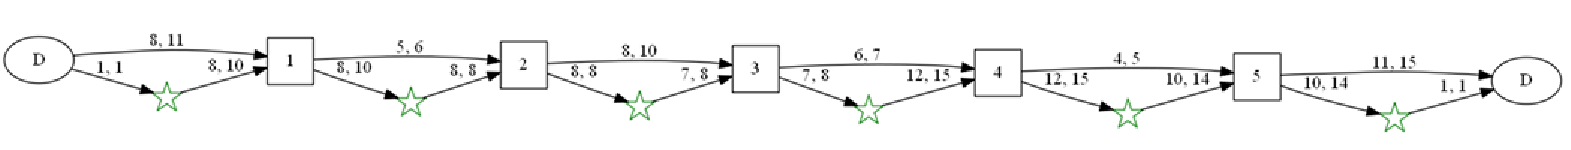
\includegraphics[height=1.7cm]{images_these/inst_Graph_J.pdf}}
	\caption[Une instance]{Une instance}
	\label{inst_Graph_J}
\end{figure}

\begin{figure}[H]
	\centerline{
		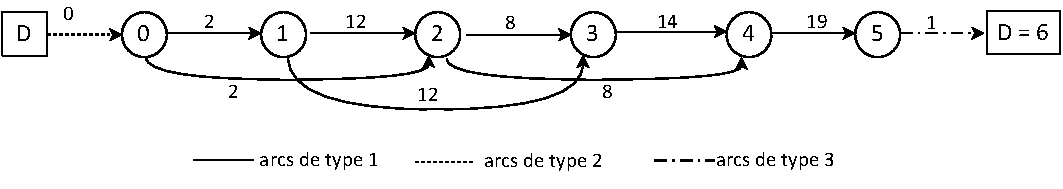
\includegraphics[height=2.9cm]{images_these/Graph_J.pdf}}
	\caption[Le graphe G]{Le graphe G correspondant à l'instance de la figure (	\ref{inst_Graph_J}) .}
	\label{Graph_J}
\end{figure}

Le plus court chemin est : $D \rightarrow 0 \rightarrow 2 \rightarrow 4 \rightarrow 5 \rightarrow 6$ de coût 30 et cela signifie que le véhicule fait le plein après le dépôt initial et après les stations 2, 4 et 5.
Pour chaque recharge, on peut calculer la quantité minimale d'hydrogène que le véhicule doit recharger pour que qu'il fasse le plein afin de pouvoir aller à la prochaine recharge (ou dépôt final). Il en résulte que :

\begin{itemize}[label=$\square$]
	\item A la première recharge, le véhicule arrive à la micro-usine avec 19 (qui correspond à $E_0- \varepsilon_0$) unités d'hydrogène dans son réservoir et il lui en faut 24 pour aller à la prochaine recharge. Il doit donc recharger 5 unités pour faire le plein.
	\item A la deuxième recharge, le véhicule arrive à la micro-usine avec 0 unité d'hydrogène dans son réservoir et il a besoin de 30 pour aller à la prochaine recharge. Il doit donc recharger 30 unités pour faire le plein.
	\item A la troisième recharge, le véhicule arrive à la micro-usine avec 0 unité d'hydrogène dans son réservoir et il lui en faut 28 pour aller à la prochaine recharge. Il doit donc recharger 28 unités pour faire le plein.
	\item A la quatrième recharge, le véhicule arrive à la micro-usine avec 0 unité d'hydrogène dans son réservoir et il lui en faut 21 pour arriver au dépôt final avec $E_0=20$ unités d'hydrogène dans son réservoir. Il doit donc recharger 21 unités pour faire le plein.
\end{itemize}
Ainsi, nous pouvons calculer la quantité totale $H$ d'hydrogène nécessaire pour toutes les recharges du véhicule.

Pour pouvoir comparer l'heuristique précédente aux autres algorithmes qui résolvent SMEPC, il faudrait  calculer un calendrier de production, c'est-à-dire décider pendant quelles périodes la micro-usine produit.
Pour ce faire, nous connaissons déjà la quantité totale $H$ d'hydrogène nécessaire à toutes les recharges du véhicule. Maintenant, nous faisons produire la micro-usine jusqu'à ce qu'au moins $H$ unités d'hydrogène aient été générées.
Plusieurs contraintes doivent être respectées :
\begin{itemize}[label=$\square$]
	\item La micro-usine ne peut pas produire lorsque le véhicule fait le plein ;
	\item La capacité du réservoir de la micro-usine ne doit jamais être dépassée, ;
	\item Le véhicule ne peut faire le plein que si la quantité d'hydrogène dans le réservoir de la micro-usine est suffisante : le véhicule attend que cette quantité soit atteinte.
\end{itemize}
Partant de la solution du problème du véhicule, pour calculer le planning de production, on utilise deux méthodes :
\begin{itemize}[label=$\square$]
	\item La première consiste à produire le plus tôt possible l'énergie $H$ que le véhicule viendra recharger ;
		\item La seconde consiste à trouver la meilleure façon de produire entre deux recharges, c'est-à-dire au coût le plus bas pour satisfaire la recharge. 
	\end{itemize}
Si la quantité d'énergie produite est insuffisante pour satisfaire le recharge, nous essayons de faire attendre le véhicule et de produire uniquement ce dont nous avons besoin pour la prochaine recharge.
On compare les solutions obtenues par ces deux méthodes et on considère que la meilleure solution est celle de l'heuristique rapide qu'on nomme $He$.
\section{Expérimentations numériques}
\label{Experimentations_num}
\subsection{Objectifs et contexte technique}

Notre objectif est d'obtenir une évaluation de l'impact des dispositifs de filtrage décrits et de la qualité des procédures gloutonnes décrites. Cet impact est à double sens : Premièrement, Il fait diminuer le nombre d'états qui sont traités tout au long du processus. Deuxièmement, l'utilisation du filtrage heuristique peut induire un gap par rapport à l'optimalité.

Les algorithmes ont été implémentés en C++ et l'IDE utilisé est Visual Studio 2017. Les expérimentations sont réalisées sur un ordinateur équipé d'un processeur AMD EPYC 7H12 64-Core, 512 Go de RAM et
fonctionnent sous Gnu/linux Ubuntu 20.04.2. Le temps maximum du CPU est fixé à 1 heure.

\subsection{Instances}
Ici, nous utilisons un ensemble de 50 instances, dont les caractéristiques sont décrites par les tableaux (\ref{tab:inst2}) et (\ref{tab:inst}).

%1 et 14(A et B)
Soient les instances A et B illustrées respectivement aux figures (\ref{Inst_0}), (\ref{tourInst_0}) et (\ref{Inst_1}), (\ref{tourInst_1}), on a illustré les solutions obtenues par l'algorithme DPS\_SMEPC. Les solutions des instances A et B sont respectivement illustrées par les figures (\ref{S_Inst_0}) et (\ref{S_Inst_1}).

	\begin{figure}[H]
	\centerline{
		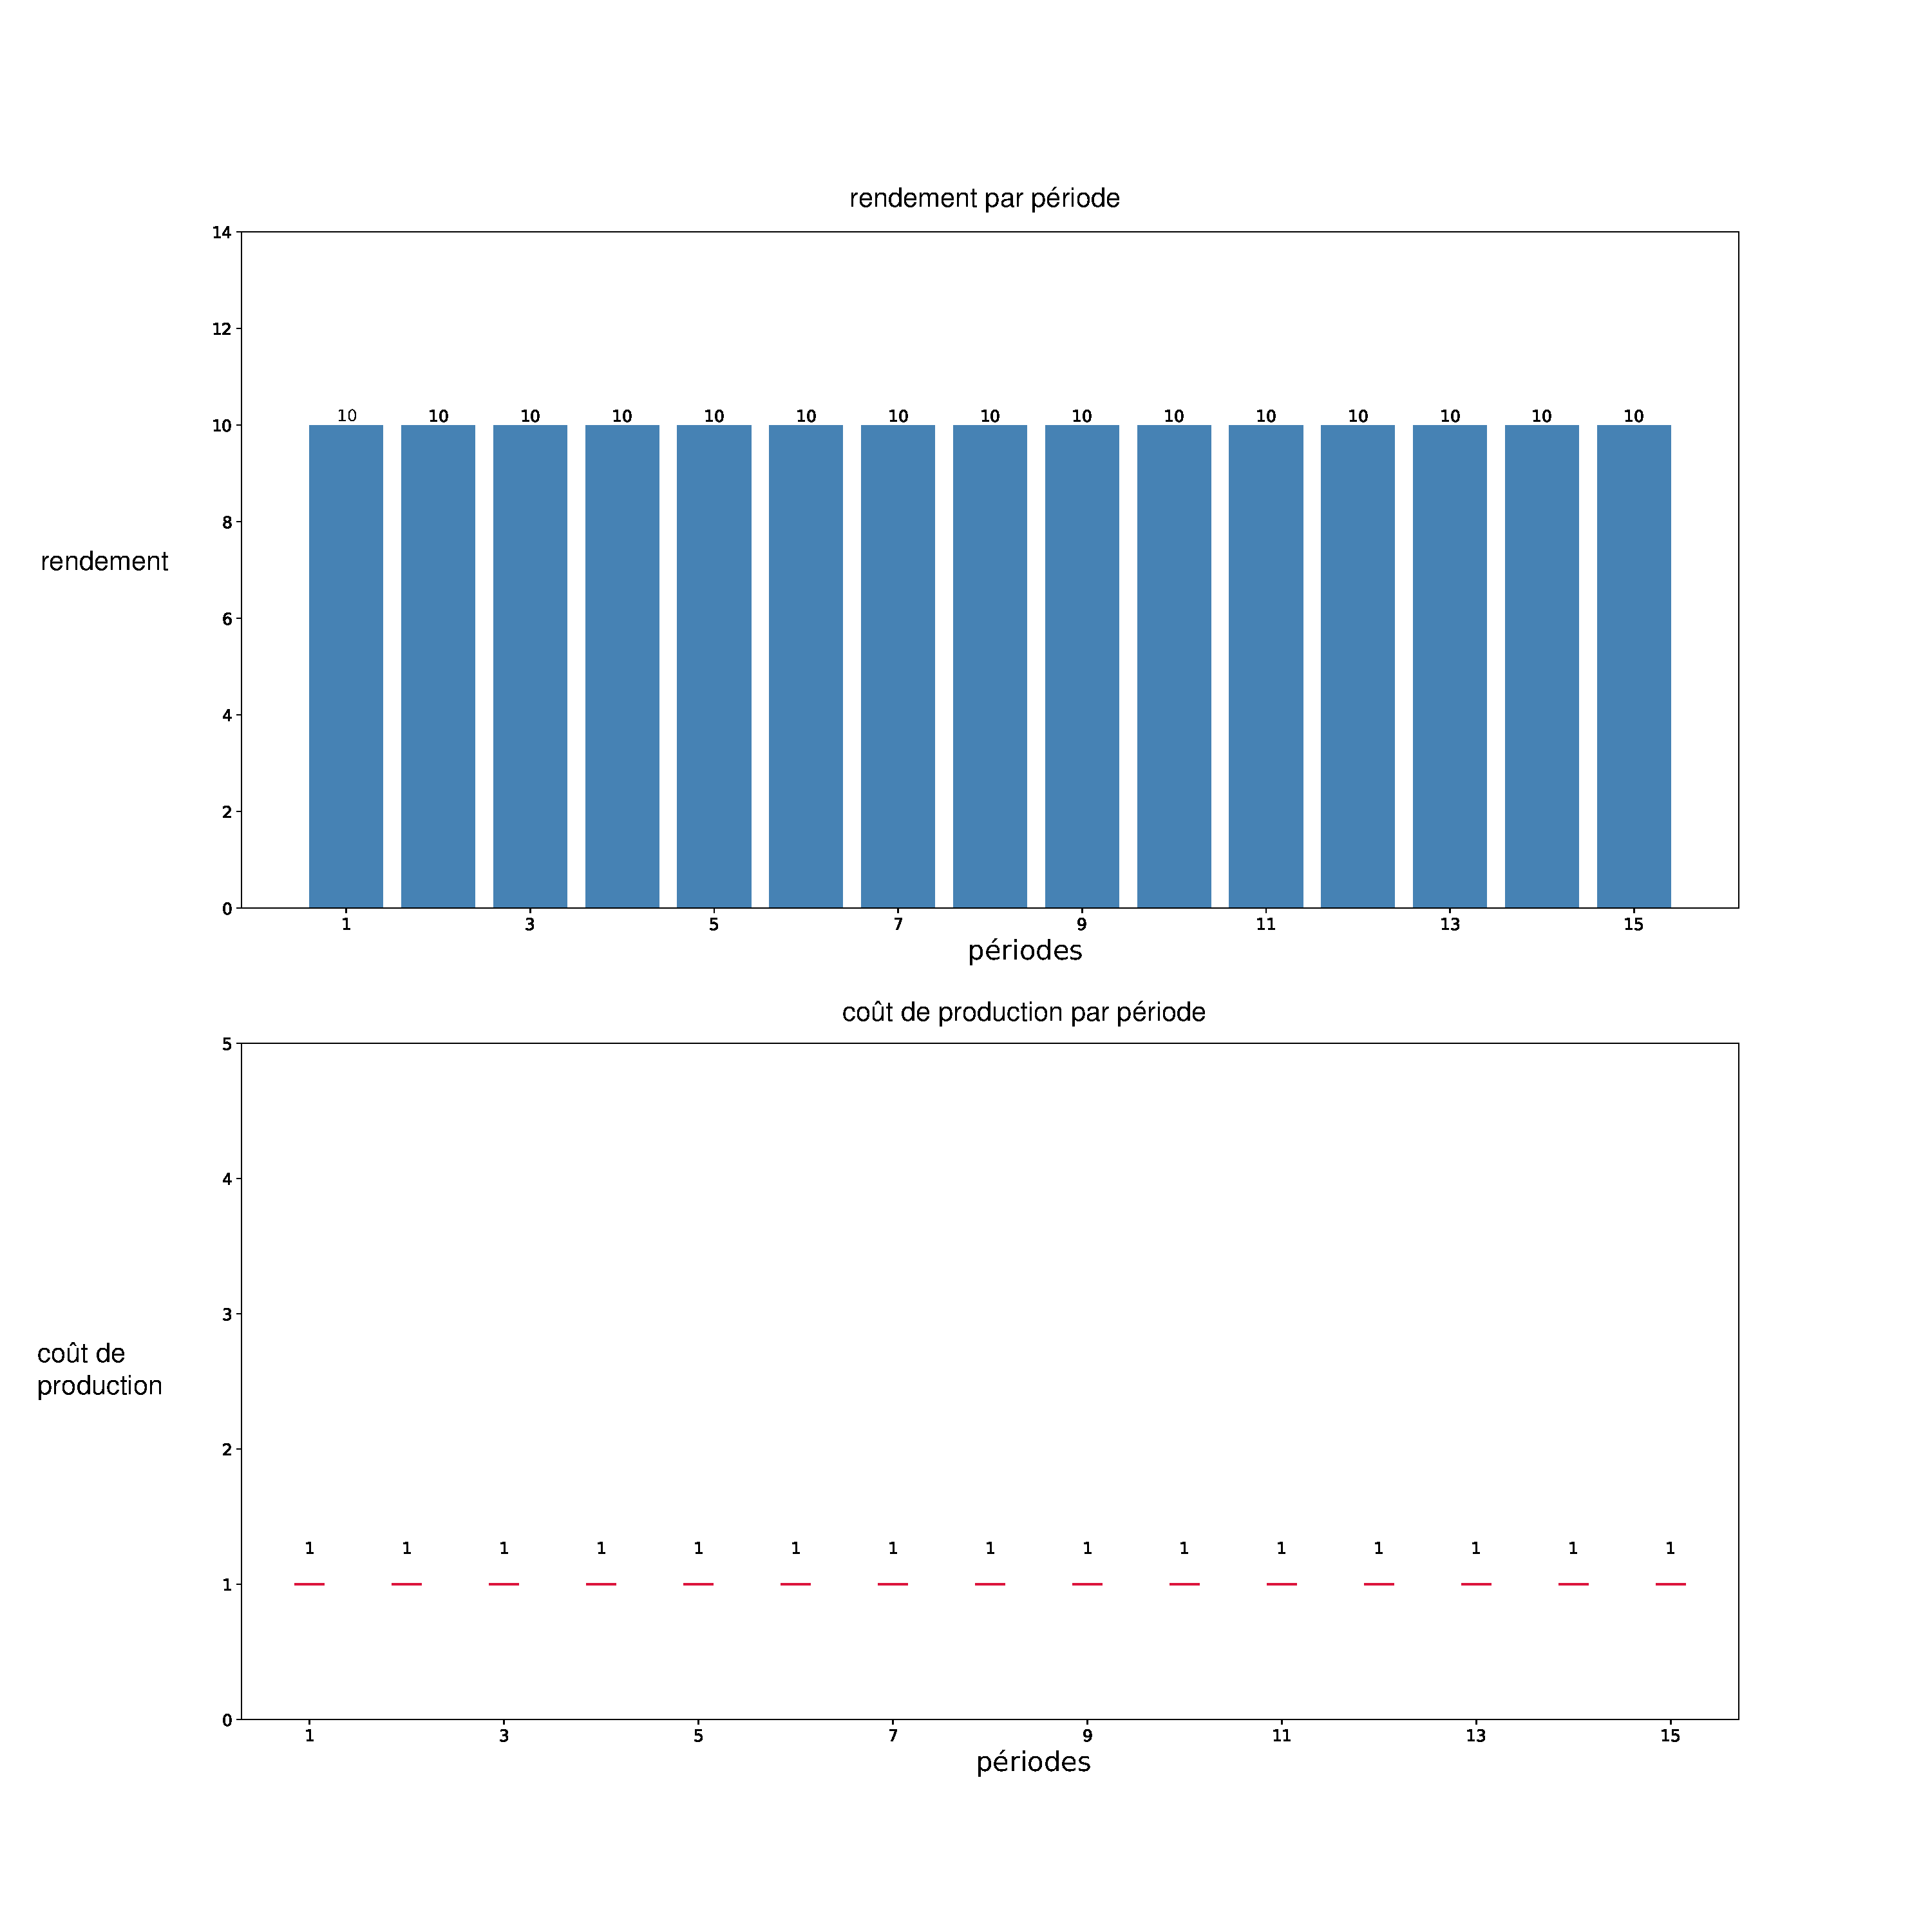
\includegraphics[height=17cm]{images_these/DPS_inputU_0.pdf}}
	\caption[Les données de la partie production de l'instance A]{Les données de la partie production de l'instance A. Sur chaque période, le rendement est 10 et le coût de production est 1.}
	\label{Inst_0}
\end{figure}
\begin{figure}[H]
	\centerline{
		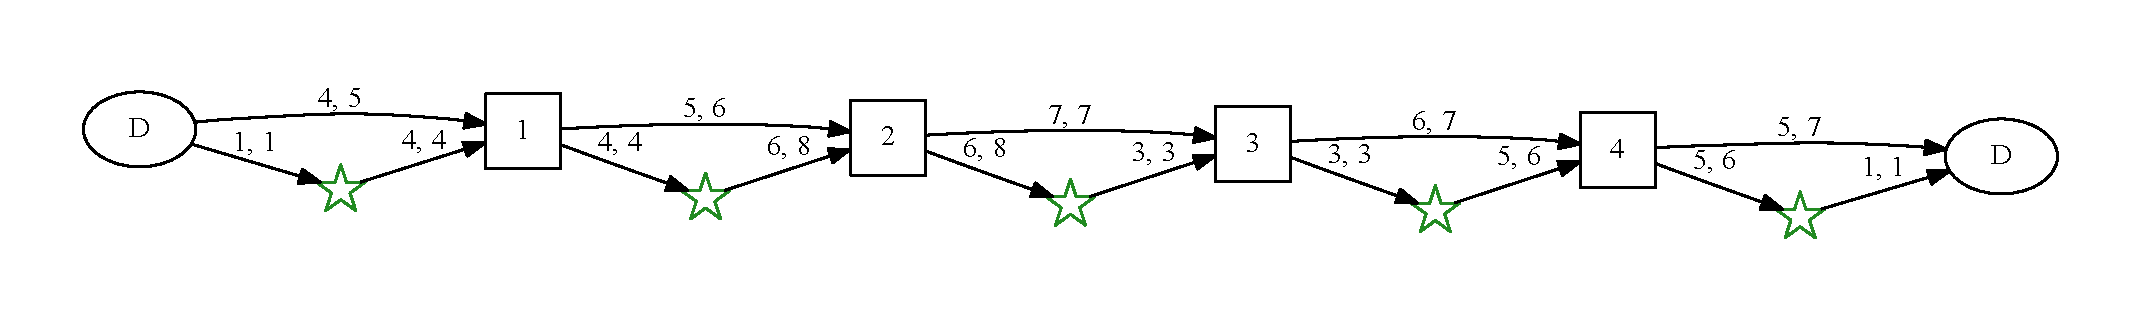
\includegraphics[height=3cm]{images_these/DPS_inputS_0.pdf}}
	\caption[Les données de la partie recharge de l'instance A]{Les données de la partie recharge de l'instance A. Les valeurs sur les arcs sont de la forme (durée, énergie).}
	\label{tourInst_0}
\end{figure}
	\begin{figure}[H]
	\centerline{
		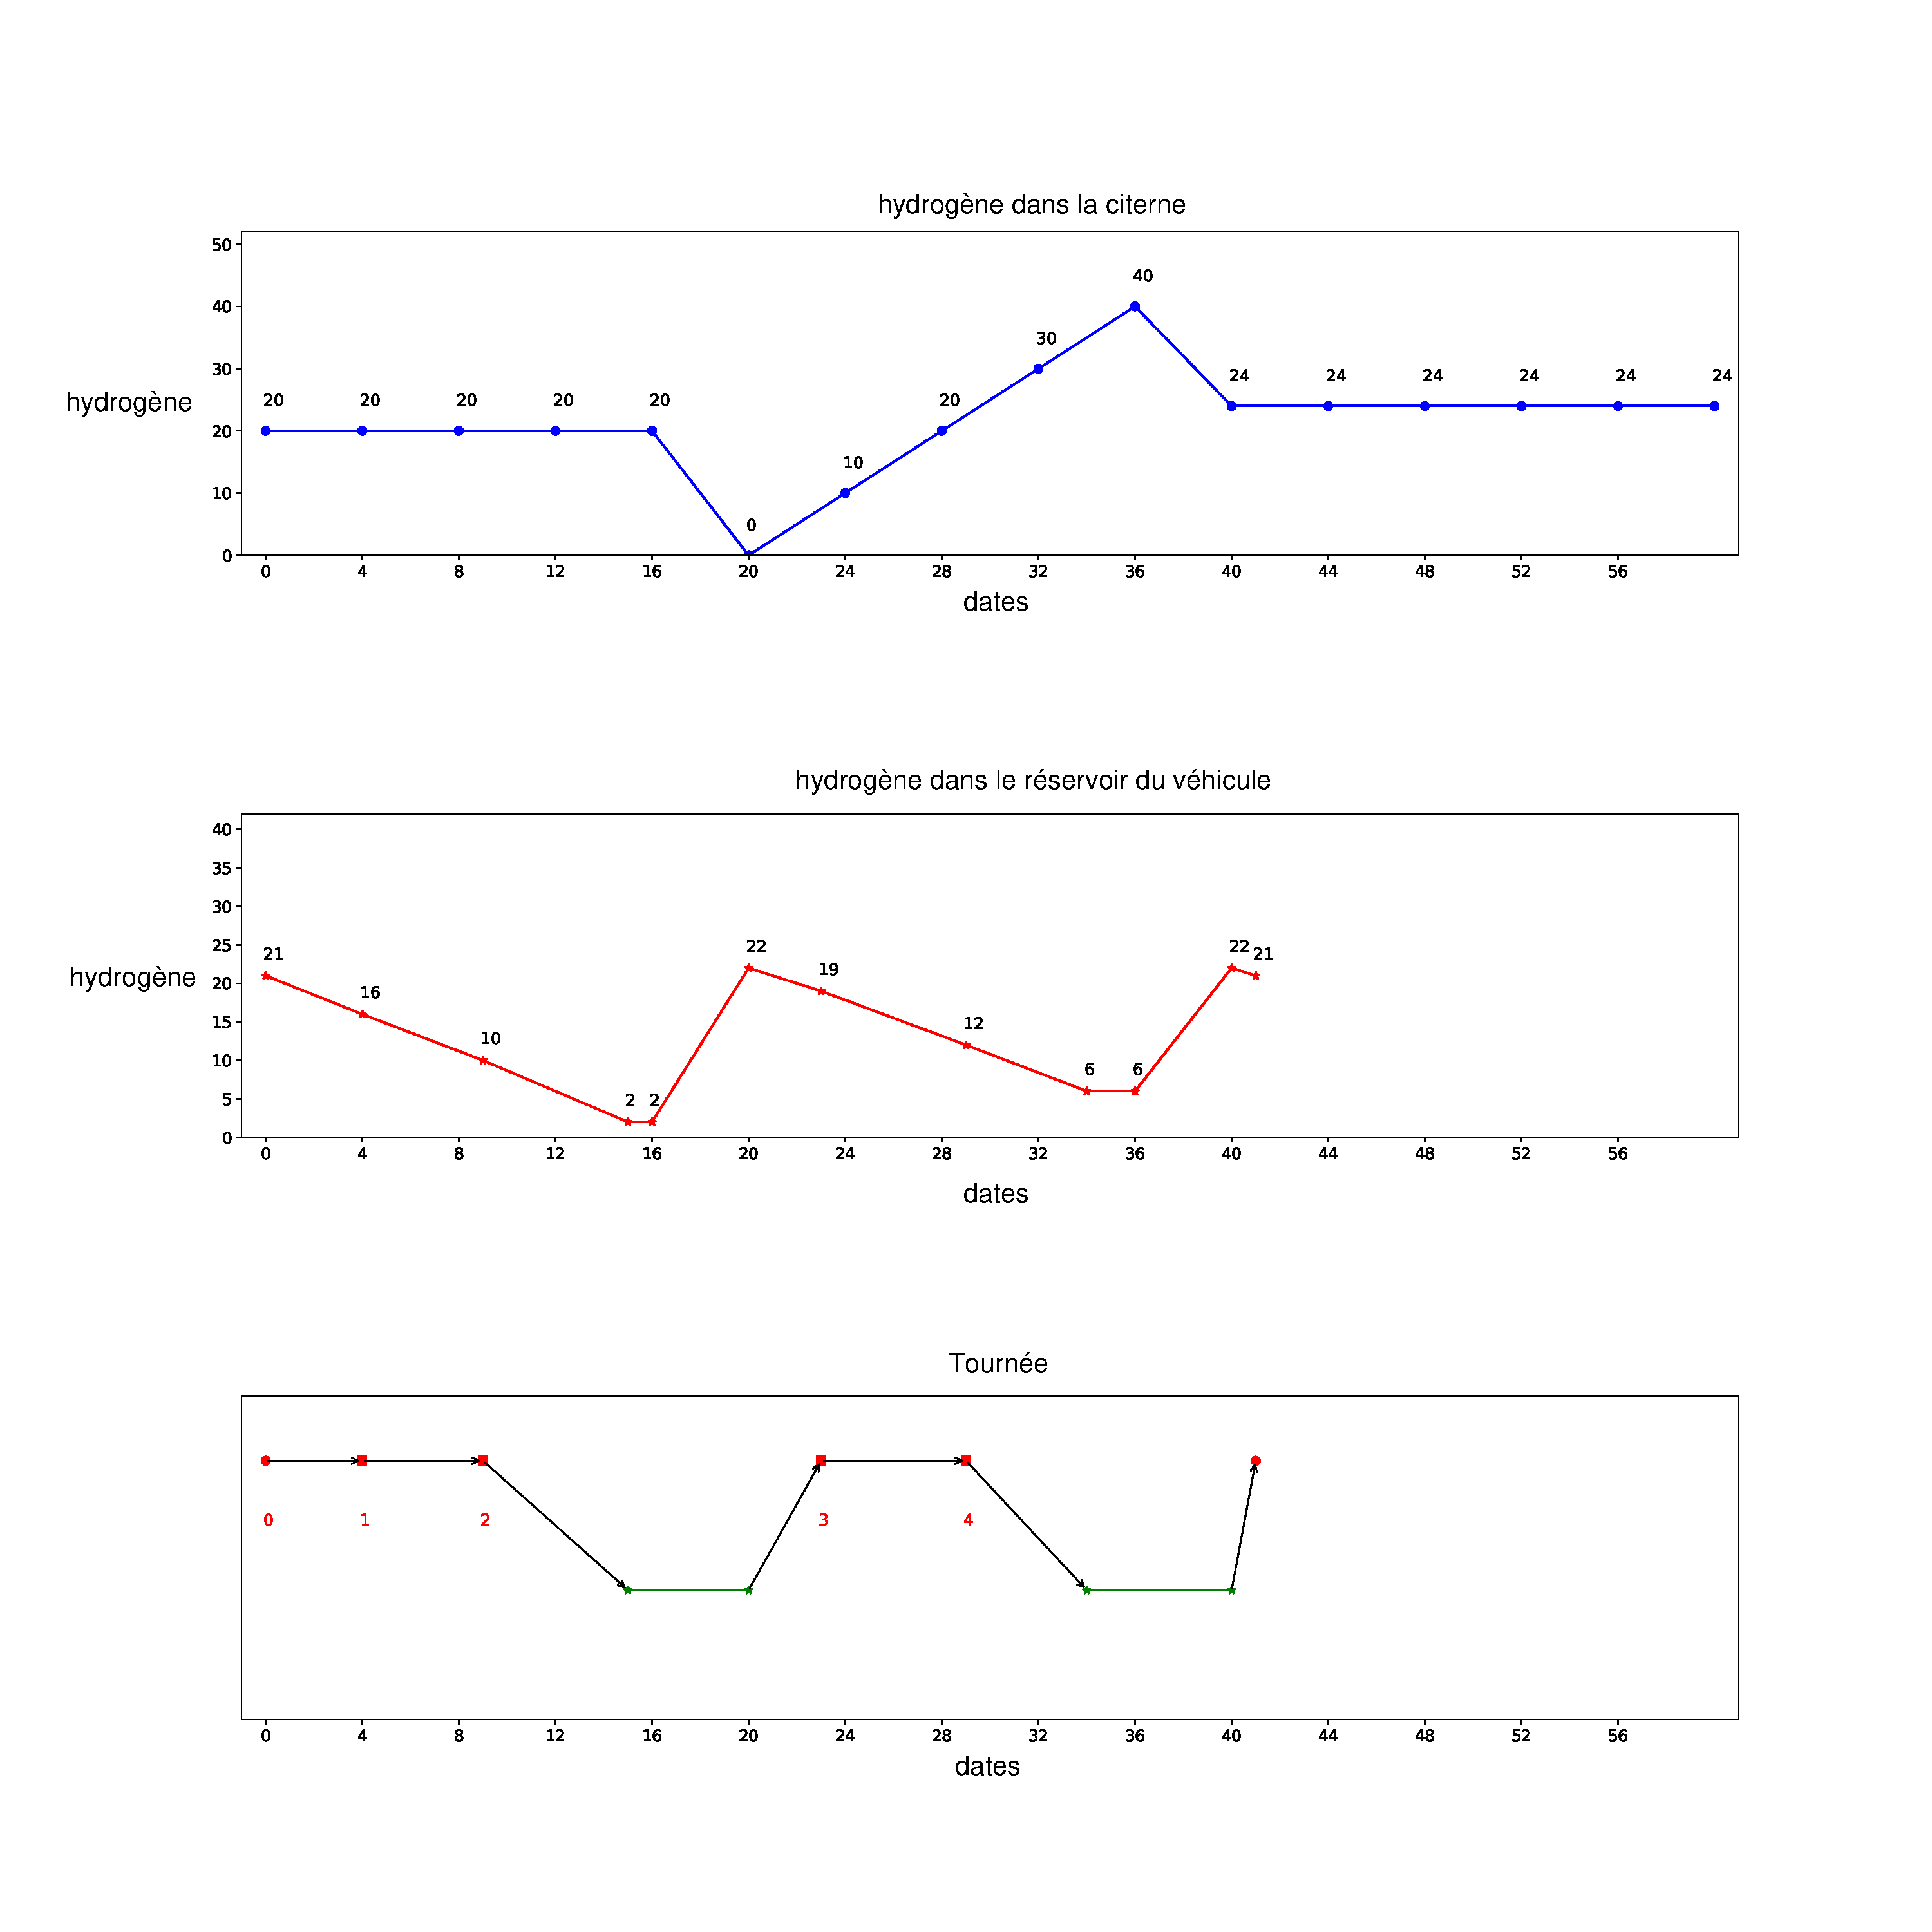
\includegraphics[height=20cm]{images_these/DPS_sol_0.pdf}}
	\caption[La solution de l'instance A]{Solution de l'instance A : on a deux recharges l'une entre la station 2 et la station 3 et l'autre entre la station 4 et le dépôt final.}
	\label{S_Inst_0}
\end{figure}
	\begin{figure}[H]
	\centerline{%trim= 1cm 15cm 1cm 9cm
		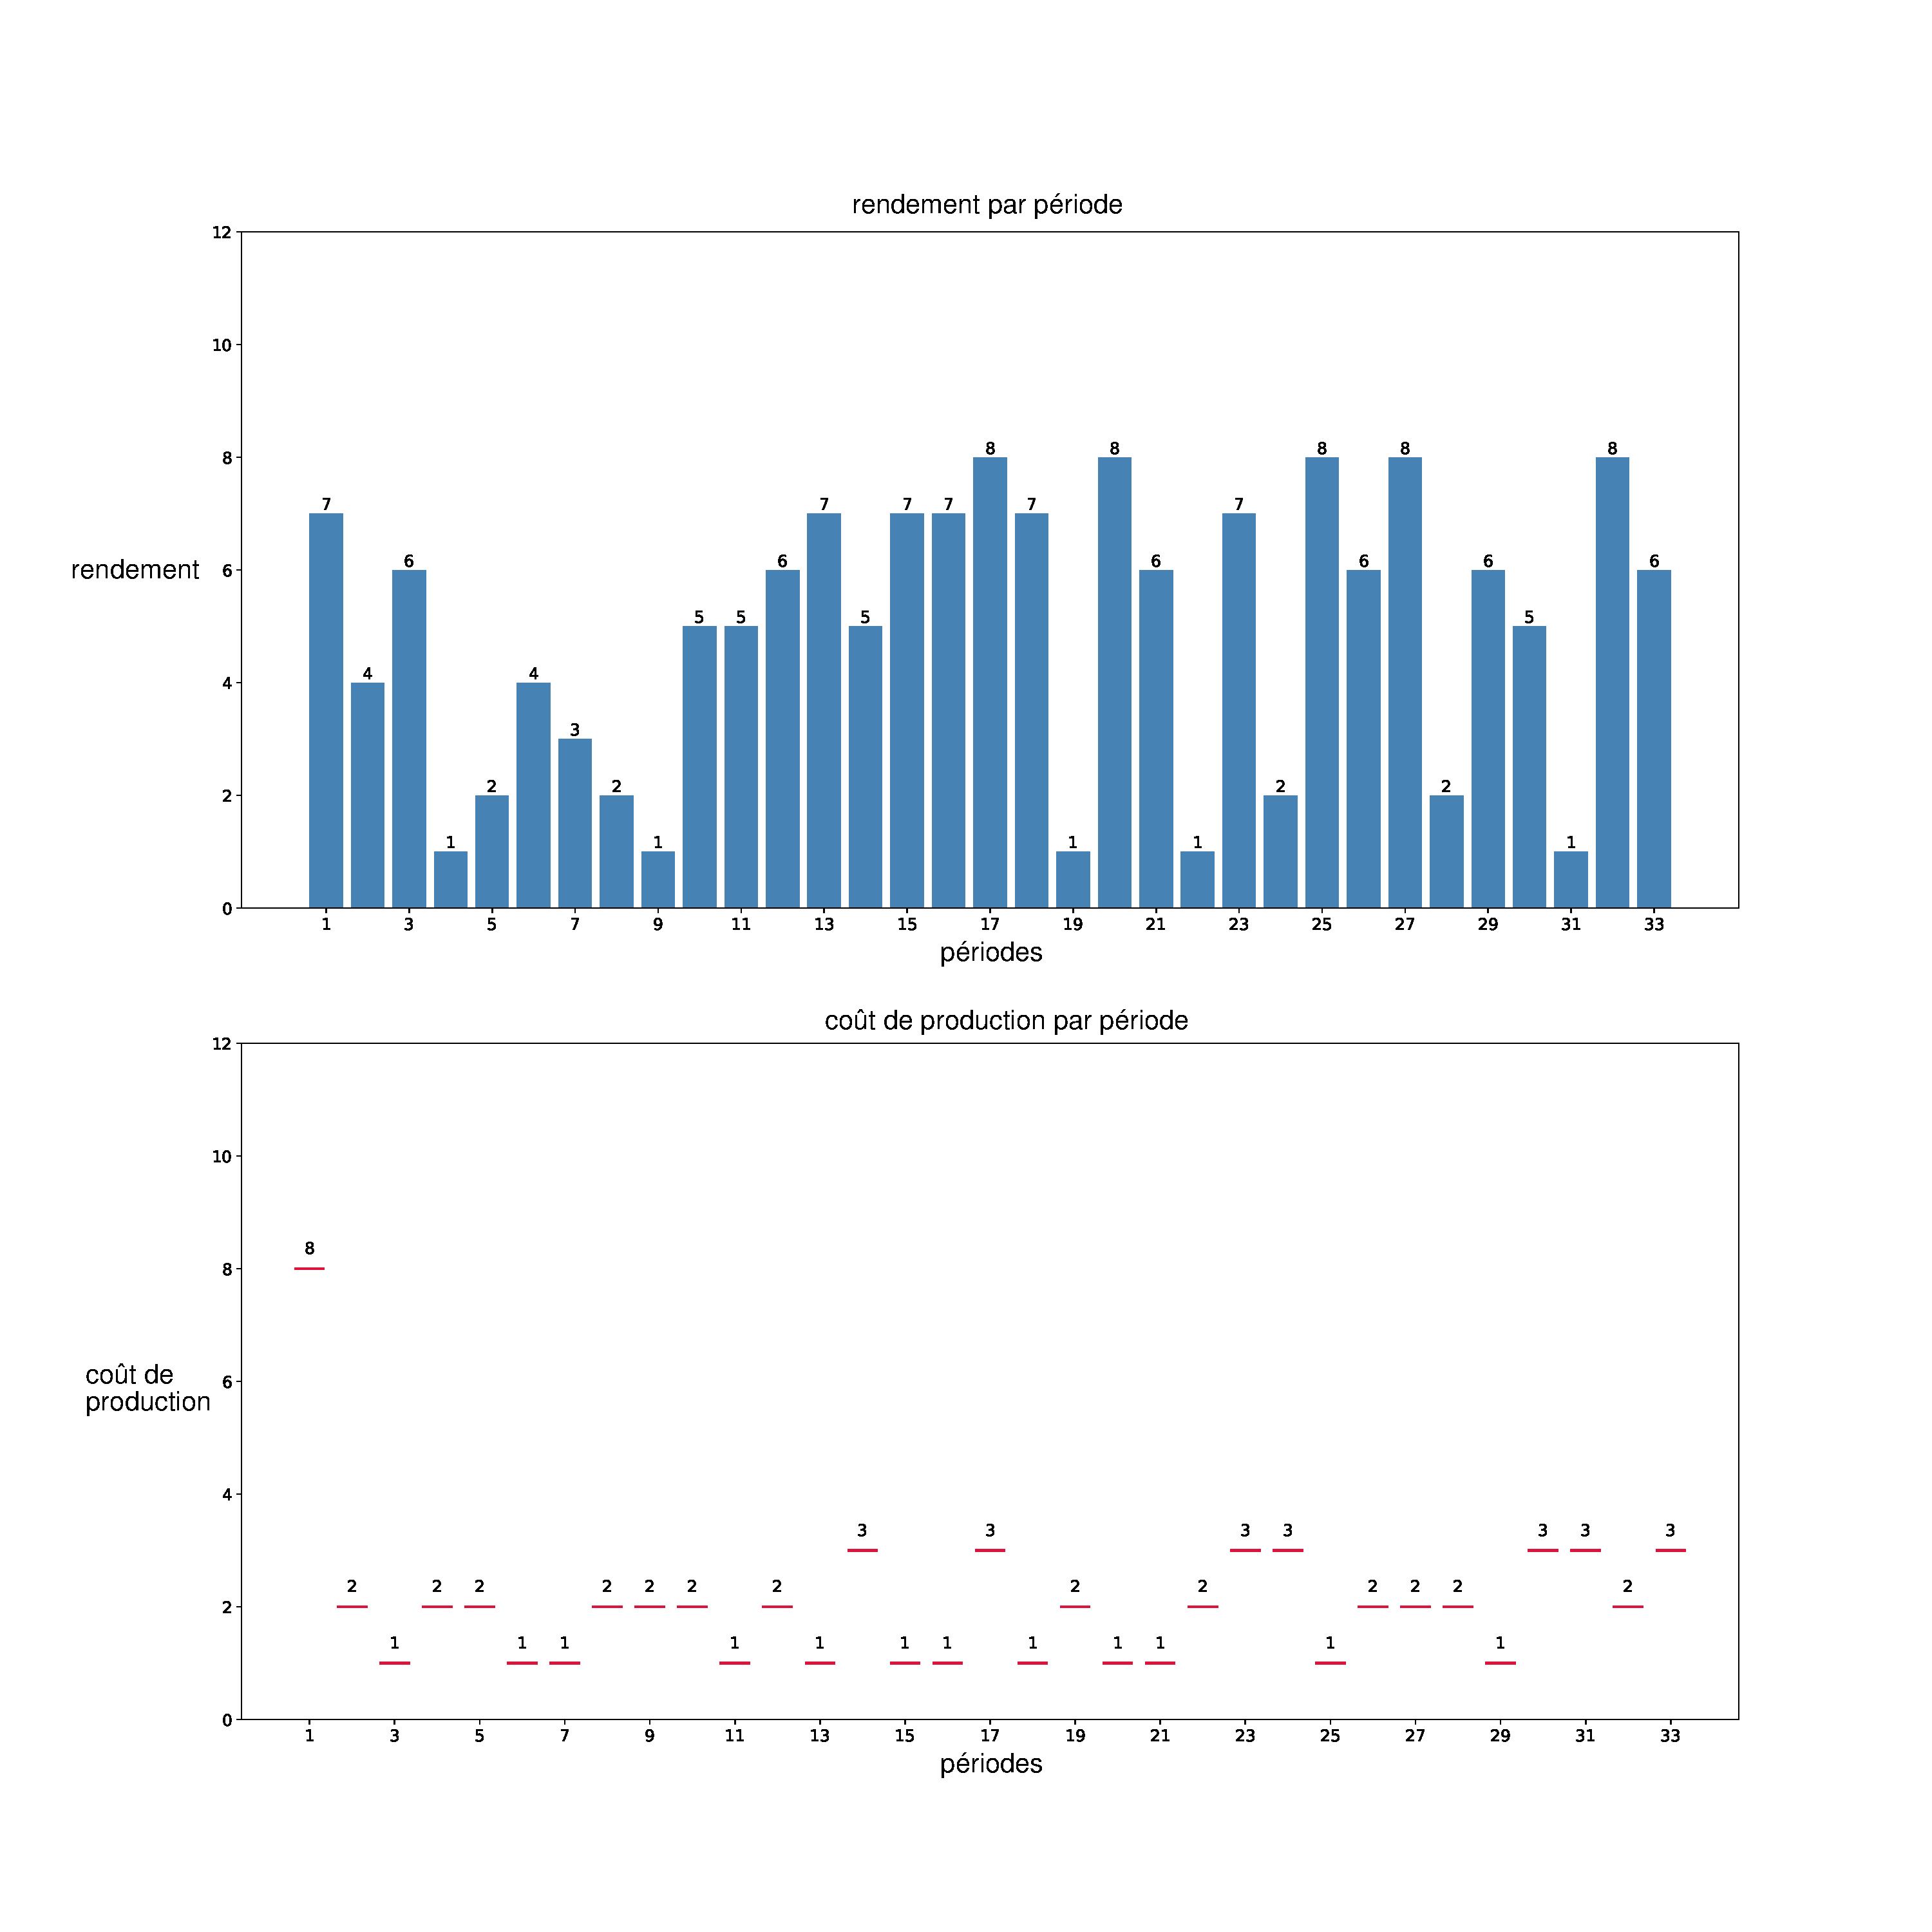
\includegraphics[height=20cm]{images_these/DPS_inputU_24.pdf}}
	\caption[Les données de la partie production de l'instance B]{Les données de la partie production de l'instance B.}
	\label{Inst_1}
\end{figure}
	\begin{figure}[H]
	\centerline{%trim= 1cm 15cm 1cm 9cm
		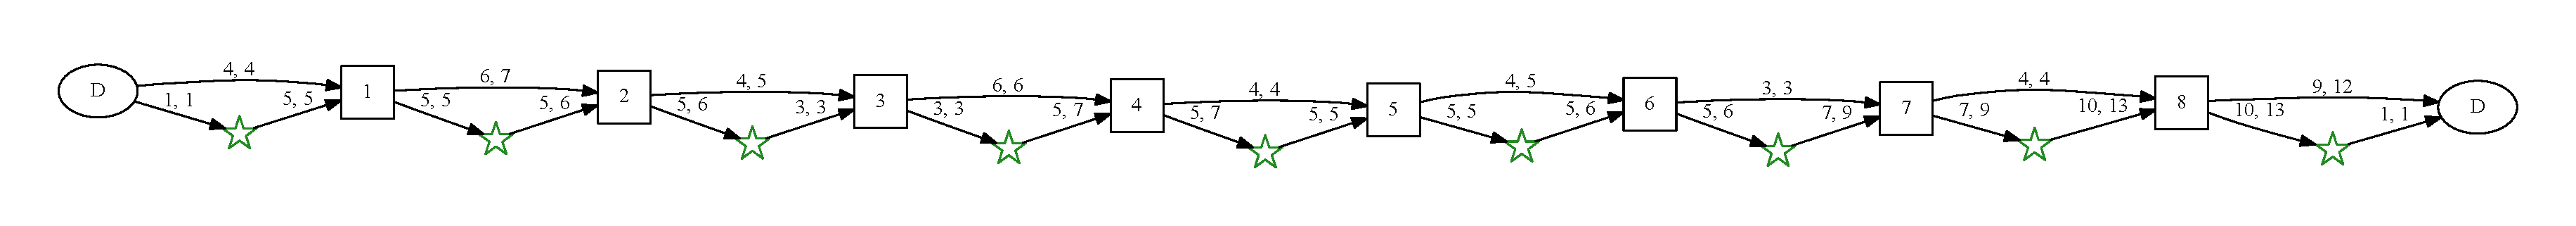
\includegraphics[height=1.9cm]{images_these/DPS_inputS_24.pdf}}
	\caption[Les données de la partie recharge de l'instance B]{Les données de la partie recharge de l'instance B. Les valeurs sur les arcs sont de la forme (durée, énergie).}
	\label{tourInst_1}
	\end{figure}
	\begin{figure}[H]
	\centerline{
		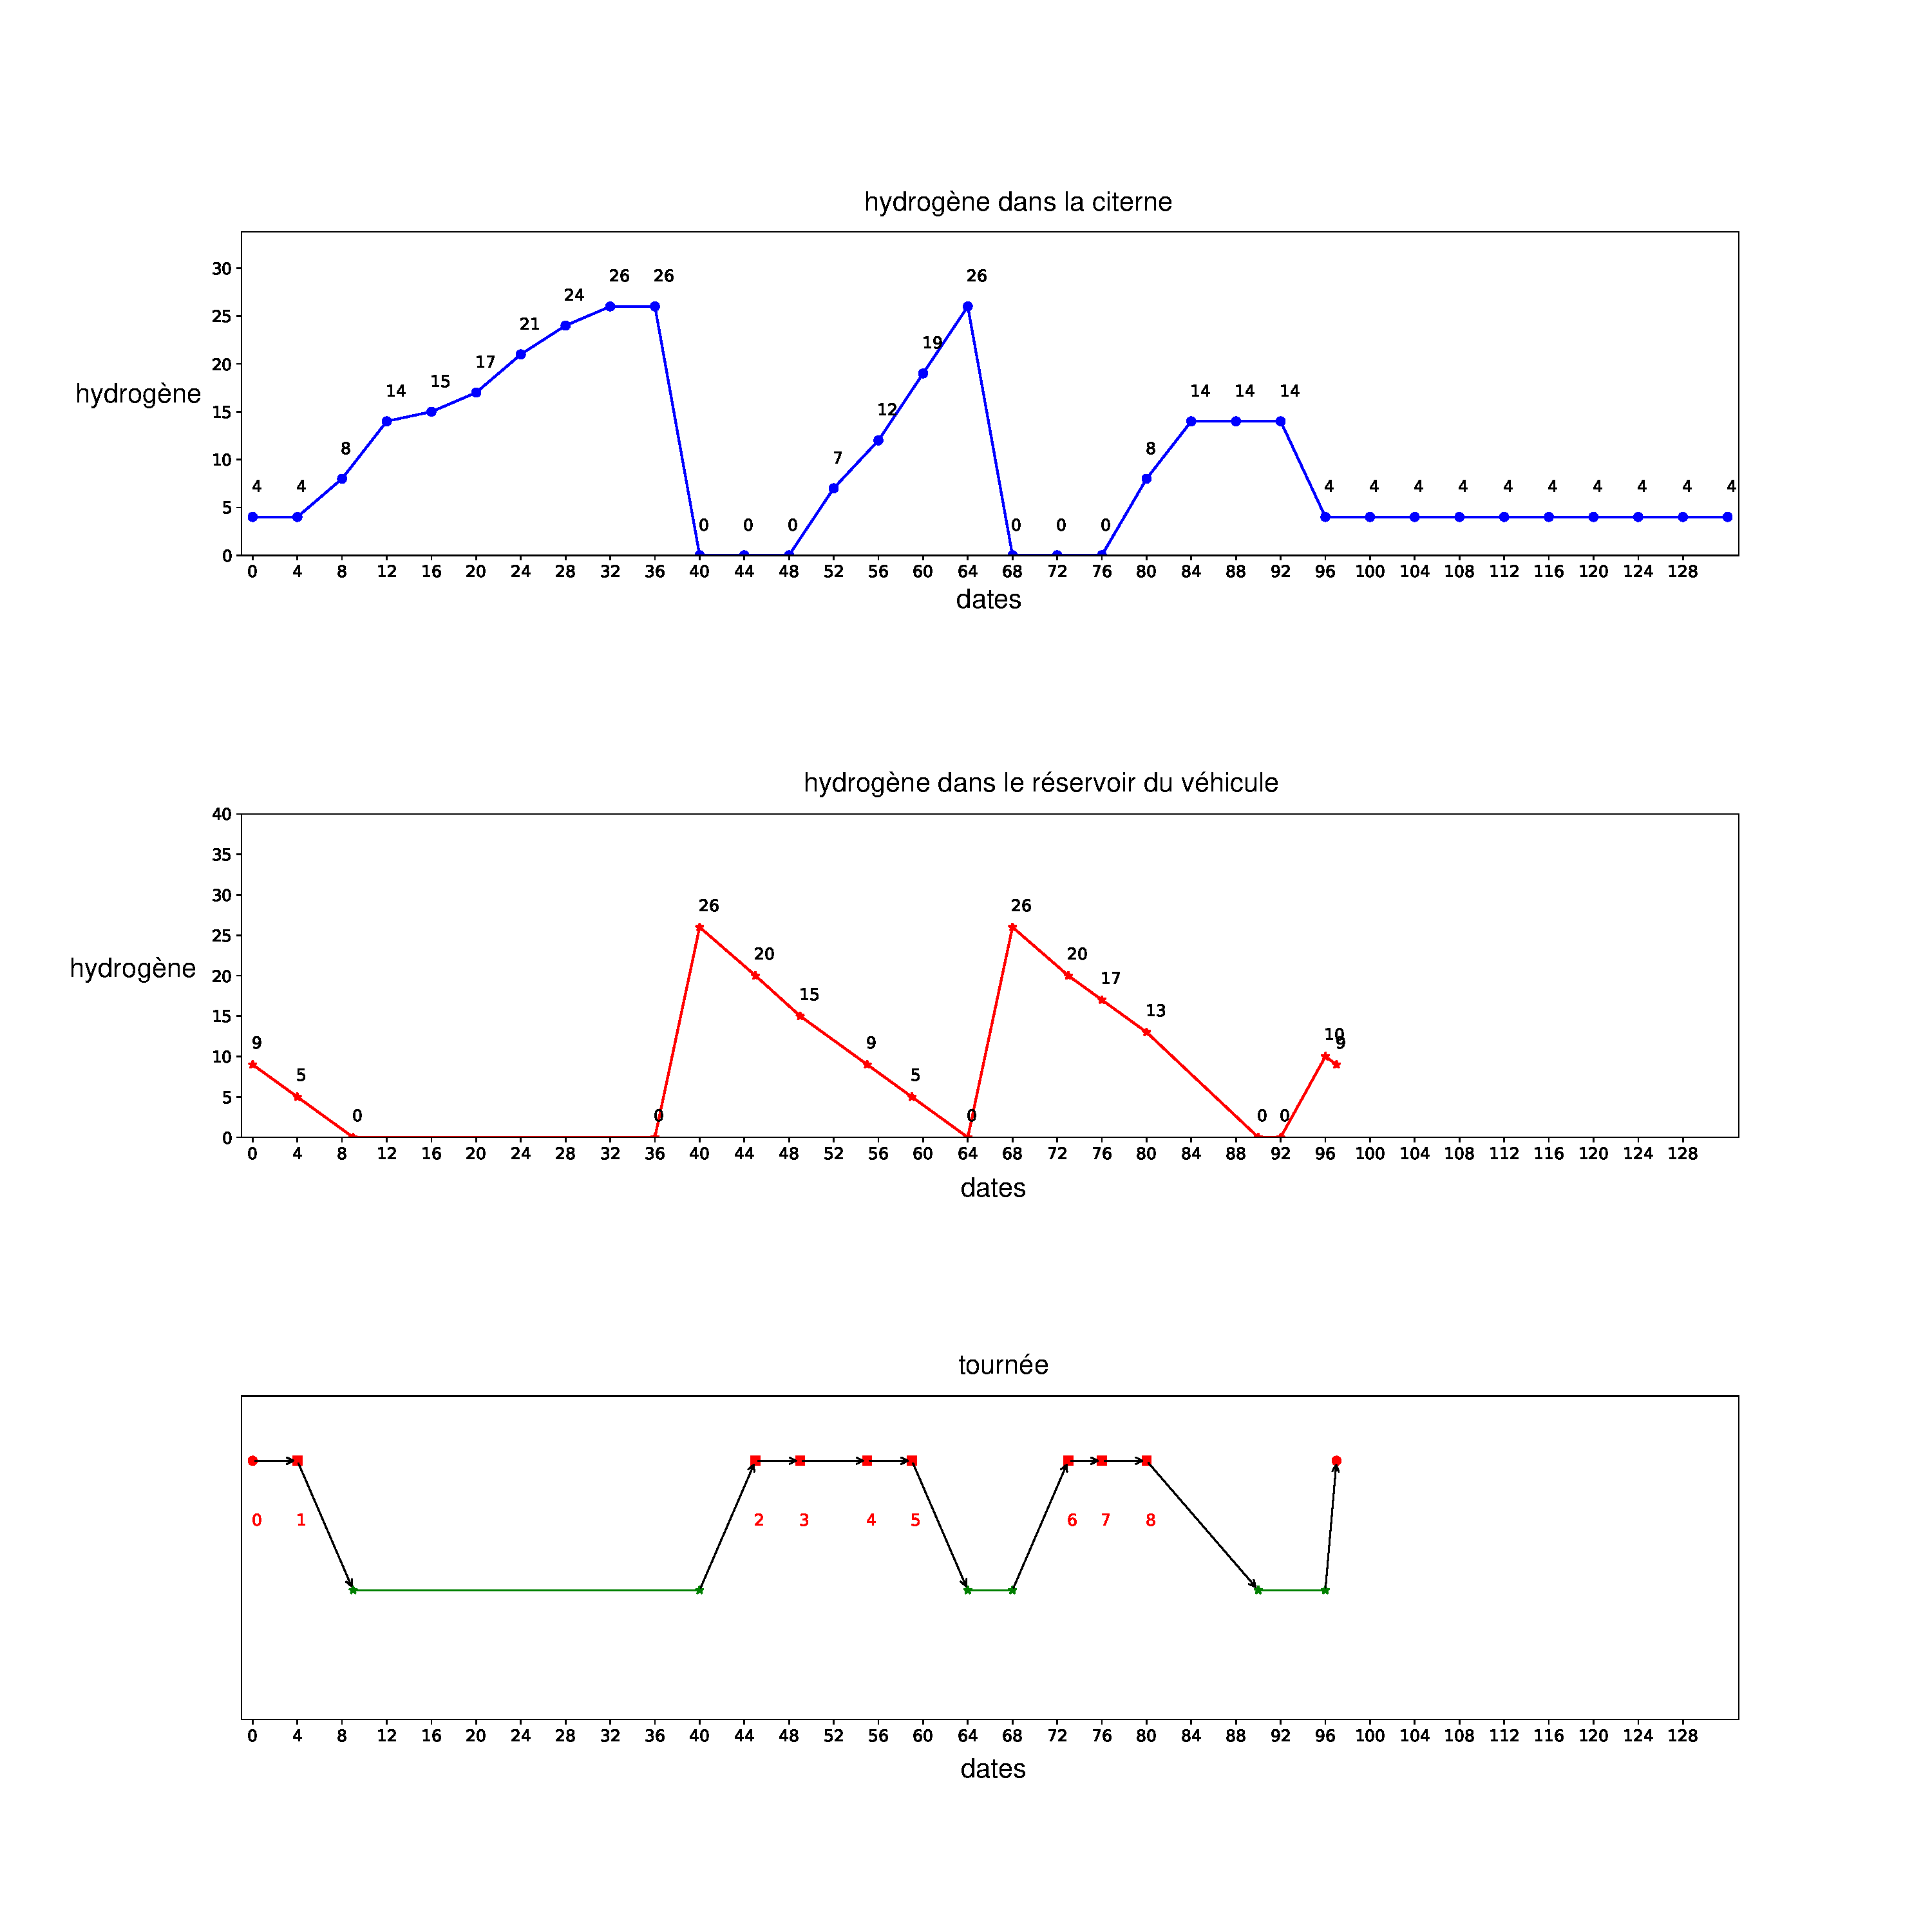
\includegraphics[height=20cm]{images_these/DPS_sol_24.pdf}}
	\caption[La solution de l'instance B]{Solution de l'instance B : on a trois recharges.}
	\label{S_Inst_1}
\end{figure}

\poubelle{
\begin{center}
	\tablefirsthead{%
	\rowcolor{cyan}	\hline\multicolumn{1}{|c|}{\tbsp Num instance}  &$N$  &  $M$ &$TMax$ &$p$  & $C^{Veh}$  & $C^{Tank}$ \\\hline}
	\tablehead{%
	\rowcolor{cyan}	\hline\multicolumn{7}{|c|}{\small\sl suite de la page précédente }\\
	\rowcolor{cyan}\hline\multicolumn{1}{|c|}{\tbsp Num instance} &$N$  &  $M$ &$TMax$ &$p$  & $C^{Veh}$  & $C^{Tank}$\\
%\hline	
}
	\tabletail{%
	\rowcolor{cyan}	\hline\multicolumn{7}{|c|}{\small\sl suite à la page suivante}\\\hline}\tablelasttail{\hline}\bottomcaption{Instances\label{Experiment_DPS-SMEPC}}
	\small
	\begin{supertabular}{|*{7}{c|}}
	%	\hline
		1&	15&	4&	60&	4&	24&	50\\ \hline
		2&	78&	10&	78&	1&	27&	27\\ \hline
		3&	94&	10&	94&	1&	17&	34\\ \hline
		4&	114&	10&	114&	1&	23&	23\\ \hline
		5&	99&	10&	99&	1&	19&	19\\ \hline
		6&	59&	10&	118&	2&	22&	22\\ \hline
		7&	36&	10&	72&	2&	19&	57\\ \hline
		8&	78&	10&	156&	2&	22&	22\\ \hline
		9&	57&	10&	114&	2&	23&	23\\ \hline
		10&	26&	8&	104&	4&	12&	36\\ \hline
		11&	26&	10&	104	&4&	15&	30\\ \hline
		12&	24&	10&	96	&4&	25&	25\\ \hline
	%	11&	26&	10&	96	&4&	25&	25\\ \hline
		13&	30&	10&	120	&4&	17&	17\\ \hline
		14&	33&	8&	132&	4&	26&	26\\ \hline
		15&	20&	8&	80	&4&	15&	30\\ \hline
		16&	25&	8&	100&	4&	21&	21\\ \hline
		17&	27&	8&	108&	4&	26&	78\\ \hline
		18&	50&	10&	200	&4&	28&	28\\ \hline
		19&	24&	10&	96&	4&	24&	72\\ \hline
		20&	44&	10&	176&	4&	20&	40\\ \hline
		21&	32&	12&	128	&4&	28&	28\\ \hline
		22&	32&	12&	128	&4&	28&	28\\ \hline
		23&	45&	14&	180	&4&	24&	24\\ \hline
		24&	30&	8&	120	&4&	29&	29\\ \hline
		25&	26&	8&	104	&4&	22&	66\\ \hline
		26&	17&	10&	68	&4&	14&	42\\ \hline
		27&	19&	10&	76	&4&	16&	48\\ \hline
		28&	20&	10&	80&	4&	27&	27\\ \hline
		29&	50&	12&	200	&4&	18&	36\\ \hline
		30&	50&	12&	200&	4&	18&	36\\ 
	\end{supertabular}
\end{center}
	
%	
\subsection{Résultats des programmes linéaires sur les instances générées}

%05/02/2021
% mettre le contenu du fichier Solution_PL_sans_new_newnew de owncloud ici.
On considère que l'ensemble des inéquations (\ref{37}), (\ref{38}), (\ref{39}) et (\ref{40}) s'appelle I1 et que l'ensemble des inéquations (\ref{42}) et (\ref{43}) s'appelle I2. Les tableaux (\ref{VALPL}) et (\ref{VALFRAC}) représentent respectivement les valeurs de \textit{$MILP_{SMEPC}$} et de \textit{$RMILP_{SMEPC}$}. Les tableaux (\ref{CPUPL}) et (\ref{CPUFRAC}) représentent respectivement les temps CPU de \textit{$MILP_{SMEPC}$} et de \textit{$RMILP_{SMEPC}$}. Les caractéristiques sont :

\begin{itemize}[label=$\square$]
	\item Val PL : valeurs de \textit{$MILP_{SMEPC}$};
	\item Val PL frac : Valeurs de \textit{$RMILP_{SMEPC}$};
	\item CPU (s) PL : Temps CPU en secondes de \textit{$MILP_{SMEPC}$};
	\item CPU (s) PL frac : Temps CPU en secondes de \textit{$RMILP_{SMEPC}$};  
\end{itemize}

\begin{center}
	\tablefirsthead{%
		\rowcolor{cyan}\hline\multicolumn{1}{|c|}{\tbsp Instance
			Id: (N, M, p)}  &Val PL&	Val PL + I1&	Val PL + I2\\
		%\hline
	}
	\tablehead{%
		\rowcolor{cyan}	\hline\multicolumn{4}{|c|}{\small\sl suite de la page précédente }\\
		\rowcolor{cyan}\hline\multicolumn{1}{|c|}{\tbsp Instance
			Id: (N, M, p)} &Val PL&	Val PL + I1&	Val PL + I2\\\hline}
	\tabletail{%
		\rowcolor{cyan}	\hline\multicolumn{4}{|c|}{\small\sl suite à la page suivante}\\\hline}\tablelasttail{\hline}\bottomcaption{Valeurs obtenues par le programme linéaire.\label{VALPL}}
	\small
	\begin{supertabular}{|*{4}{c|}}
		\hline
		1 : (15, 4, 4)&46&	46&	46\\ \hline
		2 : (78, 10, 1)& 94&	94&	94\\ \hline
		3 : (94, 10, 1)&129&	129&	129\\ \hline
		4 : (114, 10, 1)& 131&	131&	131\\ \hline
		5 : (99, 10, 1)	& 157&	157&	157\\ \hline
		6 : (59, 10, 2)& 109&	109&	109\\ \hline
		7 : (36, 10, 2)& 97&	97&	97\\ \hline
		8 : (78, 10, 2)& 140&	140&	140\\ \hline
		9 : (57, 10, 2)& 141&	141&	141\\ \hline
		10 : (26, 8, 4)	& 116&	116&	116\\ \hline
		11 : (26, 10, 4)& 133&	133&	133\\ \hline
		12 : (24, 10, 4)& 184&	184&	184\\ \hline
		13 : (30, 10, 4)& 232	&232&	232\\ \hline
		14 : (33, 8, 4)& 182&	182&	182\\ \hline
		15 : (20, 8, 4)& 81&	81&	81\\ \hline
		16 : (25, 8, 4)& 108&	108&	108\\ \hline
		17 : (27, 8, 4)& 100&	100&	100\\ \hline
		18 : (50, 10, 4)& 131&	131&	131\\ \hline
		19 : (24, 10, 4)& 102&	102&	102\\ \hline
		20 : (44, 10, 4)& 126	&126&	126\\ \hline
		21 : (32, 12, 4)& 297&	297	&297\\ \hline
		22 : (32, 12, 4)& 297&	297&	297\\ \hline
		23 : (45, 14, 4)& 305&	305	&305\\ \hline
		24 : (30, 8, 4)	& 199&	199&	199\\ \hline
		25 : (26, 8, 4)	& 141	&141&	141\\ \hline
		26 : (17, 10, 4)& 65&	65&	65\\ \hline
		27 : (19, 10, 4)& 107&	107&	107\\ \hline
		28 : (20, 10, 4)& 121&	121&	121\\ \hline
		29 : (50, 12, 4)& 202	&202&	202\\ \hline
		30 : (50, 12, 4)& 202&	202	&202\\ 
	\end{supertabular}
\end{center}

\begin{center}
	\tablefirsthead{%
		\rowcolor{cyan}	\hline\multicolumn{1}{|c|}{\tbsp Instance
			Id: (N, M, p)}  &Val PL frac&	Val PL frac + I1&	Val PL frac + I2 \\\hline}
	\tablehead{%
		\rowcolor{cyan}	\hline\multicolumn{4}{|c|}{\small\sl suite de la page précédente }\\ \rowcolor{cyan} \hline\multicolumn{1}{|c|}{\tbsp Instance
			Id: (N, M, p)} &Val PL frac&	Val PL frac + I1&	Val PL frac + I2\\\hline}
	\tabletail{%
		\rowcolor{cyan}	\hline\multicolumn{4}{|c|}{\small\sl suite à la page suivante}\\\hline}\tablelasttail{\hline}\bottomcaption{Valeurs obtenues par le modèle fractionnaire.\label{VALFRAC}}
	\small
	\begin{supertabular}{|*{4}{c|}}
		%	\hline
		1 : (15, 4, 4)&0&	30.4715&	32.100\\ \hline
		2 : (78, 10, 1)&0&	73.52&	76.936\\ \hline
		3 : (94, 10, 1)& 0&	56.9492&	62.034\\ \hline
		4 : (114, 10, 1)& 0&	69.9577&	79.012\\ \hline
		5 : (99, 10, 1)	& 0&	73.2084&	74.729\\ \hline
		6 : (59, 10, 2)& 0&	70.023&	71.554\\ \hline
		7 : (36, 10, 2)& 0&	64.2286	&64.229\\ \hline
		8 : (78, 10, 2)& 0&	73.8&	75.272\\ \hline
		9 : (57, 10, 2)& 0&	71.4381&	80.511\\ \hline
		10 : (26, 8, 4)	& 0&	42.8278	&49.168\\ \hline
		11 : (26, 10, 4)& 0&	60.8454&	64.222\\ \hline
		12 : (24, 10, 4)& 0&	91.5492	&94.358\\ \hline
		13 : (30, 10, 4)& 0&	118.239	&122.931\\ \hline
		14 : (33, 8, 4)& 0&	73.2321	&79.616\\ \hline
		15 : (20, 8, 4)& 0&	33.0567	&36.134\\ \hline
		16 : (25, 8, 4)& 0&	42.3333	&42.333\\ \hline
		17 : (27, 8, 4)& 0&	46.3057	&47.389\\ \hline
		18 : (50, 10, 4)& 0&	76.1563	&76.156\\ \hline
		19 : (24, 10, 4)& 0&	42.6987	&46.787\\ \hline
		20 : (44, 10, 4)& 0&	71.3015	&76.938\\ \hline
		21 : (32, 12, 4)& 0&	148.433	&156.555\\ \hline
		22 : (32, 12, 4)& 0&	148.433	&156.555\\ \hline
		23 : (45, 14, 4)& 0&	156.812	&163.268\\ \hline
		24 : (30, 8, 4)	& 0&	95.8937	&99.298\\ \hline
		25 : (26, 8, 4)	& 0&	50.8382	&57.608\\ \hline
		26 : (17, 10, 4)& 0&	40.8495	&42.088\\ \hline
		27 : (19, 10, 4)& 0&	52.9488	&56.894\\ \hline
		28 : (20, 10, 4)& 0&	59.4177	&62.598\\ \hline
		29 : (50, 12, 4)& 0&	108.462	&115.124\\ \hline
		30 : (50, 12, 4)& 0&	108.462	&115.124\\ 
	\end{supertabular}
\end{center}

\begin{center}
	\tablefirsthead{%
		\rowcolor{cyan}	\hline\multicolumn{1}{|c|}{\tbsp Instance
			Id: (N, M, p)}  &CPU (s) PL& 	CPU (s)PL + I1& CPU (s) PL + I2 \\\hline}
	\tablehead{%
		\rowcolor{cyan}	\hline\multicolumn{4}{|c|}{\small\sl suite de la page précédente }\\
		\rowcolor{cyan}\hline\multicolumn{1}{|c|}{\tbsp Instance
			Id: (N, M, p)} &CPU (s) PL& 	CPU (s)PL + I1& CPU (s) PL + I2\\\hline}
	\tabletail{%
		\rowcolor{cyan}	\hline\multicolumn{4}{|c|}{\small\sl suite à la page suivante}\\\hline}\tablelasttail{\hline}\bottomcaption{Temps d'exécution du programme linéaire.\label{CPUPL}}
	\small
	\begin{supertabular}{|*{4}{c|}}
		%	\hline
		1 : (15, 4, 4)&0,169&	0,081&	0,146\\ \hline
		2 : (78, 10, 1)&87,288&	0,682&	1,772\\ \hline
		3 : (94, 10, 1)& 1411,211&	23,377&	28,821\\ \hline
		4 : (114, 10, 1)& 874,916&	35,205&	23,863\\ \hline
		5 : (99, 10, 1)	& 2102,471&	239,861&	360,762\\ \hline
		6 : (59, 10, 2)& 17,103&	6,249&	5,154\\ \hline
		7 : (36, 10, 2)& 28,584&	0,568&	1,13\\ \hline
		8 : (78, 10, 2)& 676886,495&	45,935&	37,286\\ \hline
		9 : (57, 10, 2)& 52,799&	15,753&	3,488\\ \hline
		10 : (26, 8, 4)	& 1,946&	0,601&	0,983\\ \hline
		11 : (26, 10, 4)& 7,425&	1,738&	1,496\\ \hline
		12 : (24, 10, 4)& 1,14&	1,405&	1,462\\ \hline
		13 : (30, 10, 4)& 76,688&	5,849&	3,827\\ \hline
		14 : (33, 8, 4)& 23,24&	9,51&	7,667\\ \hline
		15 : (20, 8, 4)& 0,615&	0,569&	0,474\\ \hline
		16 : (25, 8, 4)& 13,381&	1,351&	2,54\\ \hline
		17 : (27, 8, 4)& 0,776&	0,431&	0,605\\ \hline
		18 : (50, 10, 4)& 20,294&	2,613&	3,638\\ \hline
		19 : (24, 10, 4)& 3,289&	0,758&	0,769\\ \hline
		20 : (44, 10, 4)& 4,326&	1,287&	1,63\\ \hline
		21 : (32, 12, 4)& 17,435&	8,335&	9,641\\ \hline
		22 : (32, 12, 4)&20,653&	7,826&	9,783\\ \hline
		23 : (45, 14, 4)&14105,918&	300,644&	691,558\\ \hline
		24 : (30, 8, 4)	&  8,758&	1,014&	1,223\\ \hline
		25 : (26, 8, 4)	&0,918&	0,49&	0,492\\ \hline
		26 : (17, 10, 4)& 0,835&	0,211&	0,387\\ \hline
		27 : (19, 10, 4)& 0,227&	0,086&	0,202\\ \hline
		28 : (20, 10, 4)& 0,261&	0,307&	0,317\\ \hline
		29 : (50, 12, 4)&  358,325&	9,763&	12,677\\ \hline
		30 : (50, 12, 4)&352,884&	10,912&	12,704\\ 
	\end{supertabular}
\end{center}

\begin{center}
	\tablefirsthead{%
		\rowcolor{cyan}	\hline\multicolumn{1}{|c|}{\tbsp Instance
			Id: (N, M, p)}  &CPU (s) PL frac&	CPU (s) PL frac + I1&	CPU (s) PL frac + I2\\\hline}
	\tablehead{%
		\rowcolor{cyan}	\hline\multicolumn{4}{|c|}{\small\sl suite de la page précédente }\\
		\rowcolor{cyan}\hline\multicolumn{1}{|c|}{\tbsp Instance
			Id: (N, M, p)} &CPU (s) PL frac&	CPU (s) PL frac + I1&	CPU (s) PL frac + I2\\\hline}
	\tabletail{%
		\rowcolor{cyan}	\hline\multicolumn{4}{|c|}{\small\sl suite à la page suivante}\\\hline}\tablelasttail{\hline}\bottomcaption{Temps d'exécution du modèle fractionnaire.\label{CPUFRAC}}
	\small
	\begin{supertabular}{|*{4}{c|}}
		%\hline	
		1 : (15, 4, 4)&0,118&	0,017&	0,019\\ \hline
		2 : (78, 10, 1)&0,075&	0,123&	0,478\\ \hline
		3 : (94, 10, 1)& 0,071&	0,182&	1,21\\ \hline
		4 : (114, 10, 1)& 0,082&	0,179&	1,041\\ \hline
		5 : (99, 10, 1)	& 0,072&	0,129&	0,77\\ \hline
		6 : (59, 10, 2)& 0,059&	0,096&	0,358\\ \hline
		7 : (36, 10, 2)& 0,031&	0,036&	0,168\\ \hline
		8 : (78, 10, 2)& 0,07&	0,112&	0,602\\ \hline
		9 : (57, 10, 2)& 0,05&	0,091&	0,298\\ \hline
		10 : (26, 8, 4)	& 0,019&	0,029&	0,066\\ \hline
		11 : (26, 10, 4)& 0,023&	0,033&	0,107\\ \hline
		12 : (24, 10, 4)& 0,027&	0,029&	0,064\\ \hline
		13 : (30, 10, 4)& 0,024&	0,059&	0,153\\ \hline
		14 : (33, 8, 4)& 0,024&	0,039&	0,081\\ \hline
		15 : (20, 8, 4)& 0,015&	0,02&	0,037\\ \hline
		16 : (25, 8, 4)& 0,022&	0,024&	0,056\\ \hline
		17 : (27, 8, 4)& 0,022&	0,024&	0,058\\ \hline
		18 : (50, 10, 4)& 0,034&	0,088&	0,255\\ \hline
		19 : (24, 10, 4)& 0,023&	0,027&	0,066\\ \hline
		20 : (44, 10, 4)& 0,033&	0,052&	0,222\\ \hline
		21 : (32, 12, 4)& 0,029&	0,042&	0,177\\ \hline
		22 : (32, 12, 4)& 0,025&	0,038&	0,173\\ \hline
		23 : (45, 14, 4)& 0,05&	0,093&	0,44\\ \hline
		24 : (30, 8, 4)	& 0,02&	0,027&	0,069\\ \hline
		25 : (26, 8, 4)	& 0,021&	0,026&	0,06\\ \hline
		26 : (17, 10, 4)& 0,017&	0,025&	0,039\\ \hline
		27 : (19, 10, 4)& 0,017&	0,029&	0,05\\ \hline
		28 : (20, 10, 4)& 0,018&	0,027&	0,057\\ \hline
		29 : (50, 12, 4)& 0,047&	0,135&	0,418\\ \hline
		30 : (50, 12, 4)& 0,048&	0,128&	0,449\\ 
	\end{supertabular}
	
\end{center}
}

\subsection{Recherche d'une borne supérieure de qualité pour le DPS\_SMEPC}%{Comparaison du Greedy-SMEPC et du DPS\_SMEPC}
\label{Borne_sup}

L'algorithme (\ref{Search_BSUP}) décrit la méthode de recherche de la borne supérieure pour le DPS\_SMEPC.
\begin{algorithm} 
	\caption{Search\_BSUP}
	\label{Search_BSUP}
	\begin{algorithmic}[1]
		
		\ENSURE BSUP
		\hline
		
		\vspace{0.3cm}
		
		\STATE Exécuter l'heuristique rapide $He$ et mettre sa valeur dans $BSUP_1$ ;
		\STATE Exécuter l'heuristique \textbf{Greedy-SMEPC}(20) avec comme borne supérieure $BSUP_1$ et mettre sa valeur dans $BSUP_2$ ;
		\STATE Exécuter l'heuristique \textbf{Greedy-SMEPC}(50) avec comme borne supérieure $Inf(BSUP_1,BSUP_2)$ et mettre sa valeur dans $BSUP_3$ ;
		\STATE Exécuter l'heuristique \textbf{Greedy-SMEPC}(100) avec comme borne supérieure $Inf(BSUP_1,BSUP_2,BSUP_3)$ et mettre sa valeur dans $BSUP_4$ ;
		\STATE $BSUP \leftarrow Inf(BSUP_1,BSUP_2,BSUP_3,BSUP_4,)$ ;
	\end{algorithmic}
\end{algorithm}

Pour pouvoir exécuter l'algorithme DPS\_SMEPC avec le filtrage par estimation optimiste on a besoin de connaitre une borne supérieure.
Pour calculer cette borne supérieure, on va exécuter plusieurs algorithmes et sélectionner la valeur la plus petite comme borne supérieure. Le premier algorithme qu'on exécute est l'heuristique rapide de la section \ref{Heuristique_rapide}. Ensuite, on exécute l'algorithme \textbf{Greedy-SMEPC}(NS) avec $NS=20$, en utilisant comme borne supérieure la valeur de l'heuristique rapide. Puis, on exécute \textbf{Greedy-SMEPC}(NS) avec $NS=50$, en utilisant comme borne supérieure la meilleure valeur entre $NS=20$ et l'heuristique rapide. Enfin, on exécute \textbf{Greedy-SMEPC}(NS) avec $NS=100$, en utilisant comme borne supérieur la meilleure valeur entre $NS=20$, $NS=50$ et l'heuristique rapide. Au final, la borne supérieure qui est utilisée pour le schéma de programmation dynamique est la meilleure valeur parmi les valeurs des algorithmes suivants : \textbf{Greedy-SMEPC}(20), \textbf{Greedy-SMEPC}(50), \textbf{Greedy-SMEPC}(100) et l'heuristique rapide.

Nous voulons obtenir une évaluation de la qualité de la procédure gloutonne \textbf{Greedy-SMEPC}(NS) décrite plus haut et de l'heuristique rapide présenté plus haut. Les tableaux (\ref{Comparaison_DPS-SMEPC_greedd}) et (\ref{Comparaison_DPS-SMEPC_greed2}) présentent respectivement les valeurs, les gaps et les temps CPU des instances du paquet INST\_CTE et du paquet INST\_VAR.  La signification des colonnes est :
\begin{itemize}[label=$\square$]
	\item  \textbf{Obj} est la valeur obtenue ;
	\item \textbf{Gap} est le gap par rapport à l'optimalité $Gap  = 100 \times \frac{ Obj-opt}{opt}$ ; où $Obj$ est la valeur obtenue et $opt$ est la valeur optimale obtenue à l'aide du modèle $MILP_{SMEPC}$ du chapitre précédent. Si une instance n'a pas été résolu jusqu'à l'optimalité, on utilise la borne supérieure de l'exécution sur 8 threads avec un temps limite de 3 heures (voir tableau (\ref{tab:resultSYM_STC}) et (\ref{tab:resultSYM_STC2})).
	\item \textbf{CPU} est le temps d'exécution en secondes. 
\end{itemize}

On recherche ici la meilleure borne supérieure qu'on utilisera lors de l'exécution de l'algorithme DPS\_SMEPC pour diminuer le nombre d'états. Pour cela, on exécute plusieurs algorithmes. Et la borne supérieure sera la meilleure valeur obtenue. La première procédure qu'on exécute est l'heuristique rapide \textbf{He}. En analysant les résultats des instances du paquet INST\_CTE, on remarque que l'algorithme \textbf{He} donne toujours une solution. En moyenne, parmi les valeurs de $NS$ testées, la procédure la plus rapide est \textbf{Greedy-SMEPC}(20) et la procédure la plus lente est \textbf{Greedy-SMEPC}(100), ce qui est normal car on garde beaucoup plus d'états.
% Cette valeur est utilisée comme borne supérieure de l'algorithme \textbf{Greedy-SMEPC}(20). %\og Lorsqu'un algorithme ne parvient pas à trouver une meilleure solution que sa borne supérieure, on considère que sa valeur est sa borne supérieure. \fg{}

Pour le paquet d'instances INST\_CTE et le paquet d'instances INST\_VAR on fait les remarques suivantes : 
\begin{itemize}[label=$\square$]
\item On remarque que lorsqu'on augmente la valeur de $NS$, on obtient de meilleures solutions, ce qui est surement dû au fait que la valeur de la procédure exécutée précédemment est utilisée comme borne supérieure de la procédure suivante. 
\item On constate qu'il y a une amélioration de la valeur et cela s'accompagne d'une augmentation du temps de calcul, car on augmente le nombre d'états qu'on garde.	

\item La rapidité d'exécution de la procédure \textbf{Greedy-SMEPC}(NS) peut être dû à l'efficacité de l'heuristique rapide \textbf{He}. 										
\end{itemize}
%Nous exécutons d'abord Greedy-SMEPC abrégé $GS$ et calculons le gap $GAP\_GS$ entre la solution $GS$ obtenue et la solution optimale. Ensuite, nous exécutons également le \textbf{DPS\_SMEPC} avec la mécanisme de filtrage par relation dominance faible ainsi que les autres mécanismes de filtrage, de telle sorte que le nombre d'états est toujours contrôlé en dessous d'un certain seuil $NS$ à chaque pas de temps au sens de la programmation dynamique, et nous nous concentrons sur le gap  $GAP\_GS(NS)$ entre la solution obtenue et la solution optimale. Par exemple, dans le cas où NS vaut 100, le gap vaut $GAP\_GS(100)  = (GS(100) -  ValDPS\_SMEPC)/ ValDPS\_SMEPC$.
%Nous désignons par $GS(NS)$ la valeur induite par cette dernière procédure. ValDPS\_SMEPC est la valeur de \textbf{DPS\_SMEPC}. Ici -1 signifie que l'algorithme n'a pas fournit de résultat.
\poubelle{
	\begin{center}
		\tablefirsthead{%
			\hline
			\rowcolor{cyan}	\multicolumn{1}{|c|}{\tbsp Instance
				Id: (N, M, p)}    & ValDPS\_SMEPC &  GS(1) &GS(50) &GS(100)&	GAP\_GS(100) \\\hline}
		\tablehead{%
			\hline
			\rowcolor{cyan}\multicolumn{6}{|c|}{\small\sl suite de la page précédente }\\
			\rowcolor{cyan}\hline\multicolumn{1}{|c|}{\tbsp Instance
				Id: (N, M, p)}    &  DPS\_SMEPC &  GS(1) &GS(50) &GS(100)&	GAP\_GS(100) \\\hline}
		\tabletail{%
			\rowcolor{cyan}	\hline\multicolumn{6}{|c|}{\small\sl suite à la page suivante}\\\hline}\tablelasttail{\hline}\bottomcaption{Comparaison du DPS\_SMEPC et du Greedy-SMEPC.\label{Comparaison_DPS-SMEPC_greed}}
		\small
		\begin{supertabular}{|*{6}{c|}}
			%\hline
			1 : (15, 4, 4)&	46&	-1&	46&	46&	0\\
			\hline
			2 : (78, 10, 1)&	94&	-1&	127&	103&	9,57 \\
			\hline
			3 : (94, 10, 1)&	129&	-1&	173&	141&	9,30 \\
			\hline
			4 : (114, 10, 1)&	131&	-1&	150&	144	&9,92 \\
			\hline
			5 : (99, 10, 1)	&157&	-1&	165&	163&	3,82 \\
			\hline
			6 : (59, 10, 2)&	109&	-1&	117&	113&	3,66 \\
			\hline
			7 : (36, 10, 2)&	97&	173&	133&	97&	0\\
			\hline
			8 : (78, 10, 2)&140&	-1&	141&	176&	25,7 \\
			\hline
			9 : (57, 10, 2)&	141&	-1&	154&	150&	6,38 \\
			\hline
			10 : (26, 8, 4)&	116&	-1&	116&	116&	0\\
			\hline
			11 : (26, 10, 4)&	133&	-1&	171&	133&	0\\
			\hline
			12 : (24, 10, 4)&	184&	-1&	188&	-1&	-1\\
			\hline
			13 : (30, 10, 4)&	232&	-1&	248&	248&	6,89 \\
			\hline
			14 : (33, 8, 4)&	182&	-1&	207	&201&	10,4 \\
			\hline
			15 : (20, 8, 4)&	81&	-1&	87&	81&	0\\
			\hline
			16 : (25, 8, 4)&	108&	-1&	119	&108&	0\\
			\hline
			17 : (27, 8, 4)&	100&	102&	100	&100&	0\\
			\hline
			18 : (50, 10, 4)&	131&	182	&140&	139&	6,10 \\
			\hline
			19 : (24, 10, 4)&	102&	-1&	145&	102&	0\\
			\hline
			20 : (44, 10, 4)&	126&	-1&	135&	126&	0\\
			\hline
			21 : (32, 12, 4)&	297	&-1&	314&	305	&2,69 \\
			\hline
			22 : (32, 12, 4)&	297&	-1&	314	&305&	2,69 \\
			\hline
			23 : (45, 14, 4)&	305&	-1&	350	&309&	1,31 \\
			\hline
			24 : (30, 8, 4)&	199	&-1	&242&	199&	0\\
			\hline
			25 : (26, 8, 4)&	141&	-1&	169&	141&	0\\
			\hline
			26 : (17, 10, 4)&	65&	-1&	65	&65&	0\\
			\hline
			27 : (19, 10, 4)&	107&	-1&	124	&107&	0\\
			\hline
			28 : (20, 10, 4)&	121&	-1&	122&	121&	0\\
			\hline
			29 : (50, 12, 4)&	202&	-1&	261&	202&	0\\
			\hline
			30 : (50, 12, 4)&	202	&-1	&261&	46&	0\\
			
		\end{supertabular}
	\end{center}
}


%%%%%%%%%%%%%%%%%%%%%%%%%%%%%%%%%%%%%%%%%%%%%%%%%%
\subsubsection{Recherche d'une borne supérieure de qualité pour le DPS\_SMEPC : les instances du paquet INST\_VAR}
%En analysant les résultats des instances du paquet INST\_VAR, on remarque que l'algorithme \textbf{He} donnent toujours une solution. Lorsqu'un algorithme ne parvient pas à trouver une meilleure solution que sa borne supérieure, on considère que sa valeur est sa borne supérieure. Les valeurs de gaps absentes sont les instances dont on ne connait pas la valeur optimale. On remarque que lorsqu'on augmente la valeur de $NS$, on obtient de meilleures solutions. Le temps d'exécution de tous les algorithmes est toujours inférieur à 0,6 seconde. La rapidité d'exécution de la procédure \textbf{Greedy-SMEPC}(NS) peut être dû à l'efficacité de l'heuristique rapide \textbf{He}.

%On recherche ici la meilleure borne supérieure qu'on utilisera lors de l'exécution de l'algorithme DPS\_SMEPC. Pour cela, on exécute plusieurs algorithmes à la queue leu-leu. Et la borne supérieure sera la meilleure valeur obtenue. La première procédure qu'on exécute est \textbf{He}. En analysant les résultats des instances du paquet INST\_VAR, on remarque que l'algorithme \textbf{He} donne toujours une solution. Cette valeur est utilisée comme borne supérieure de l'algorithme \textbf{Greedy-SMEPC}(20). Lorsqu'un algorithme ne parvient pas à trouver une meilleure solution que sa borne supérieure, on considère que sa valeur est sa borne supérieure. 
%Les valeurs de gaps absentes sont les instances dont on ne connait pas la valeur optimale.

 %La rapidité d'exécution de la procédure \textbf{Greedy-SMEPC}(NS) peut être dû à l'efficacité de l'heuristique rapide \textbf{He}.
  %On remarque que lorsqu'on augmente la valeur de $NS$, on obtient de meilleures solutions, ce qui est surement dû au fait que la valeur de la procédure exécutée précédemment est utilisée comme borne supérieure de la procédure suivante.
  Le tableau (\ref{Comparaison_DPS-SMEPC_greedd}) présente les résultats du calcul d'une borne supérieure de qualité pour les instances du paquet INST\_VAR. 
   Le temps d'exécution de tous les algorithmes est toujours inférieur à 0,7 seconde.
   
  %Ici, \textbf{Greedy-SMEPC}(50) est en moyenne plus rapide que l'heuristique \textbf{He}.
  % Globalement le gap moyen de \textbf{He}, \textbf{Greedy-SMEPC}(20), \textbf{Greedy-SMEPC}(50), \textbf{Greedy-SMEPC}(100) est respectivement 20,315 ; 12,6581	; 6,9131 ; 4,2625 et le temps d'exécution moyen en seconde est respectivement 0,007 ; 0,032 ; 0,066 ; 0,1268. On a calculé la moyenne des gaps seulement sur les 16 premiers instances. La valeur moyenne de \textbf{He}, \textbf{Greedy-SMEPC}(20), \textbf{Greedy-SMEPC}(50), \textbf{Greedy-SMEPC}(100) est respectivement 1576,5 ; 1563,533 ; 1548,833 ; 1538,4. %On constate qu'il y a une amélioration de la valeur et cela s'accompagne d'une augmentation du temps de calcul, car on augmente le nombre d'états qu'on garde. 
  		
  		
  		
  		
  									
%%%%%%%%%%%%%%%%%%%%%%%%%%%%%%%%%%%%%%%%%%%%%%%%%%%%%%%%%%%%%%%%%%%%%%%%%%%%%%%%%%%%%%%%%
\begin{table}[H]
	\centering
	\small
	\begin{tabular}{|r|rrr|rrr|rrr|rrr|}
		\toprule
		\hline
		\rowcolor{cyan}	& \multicolumn{3}{c|}{\textbf{He}}&\multicolumn{3}{c|}{\textbf{NS(20)}}&\multicolumn{3}{c|}{\textbf{NS(50)}}&\multicolumn{3}{c|}{\textbf{NS(100)}} \\ \hline
		\midrule
		\rowcolor{cyan}	\textbf{num} & \textbf{Obj}& \textbf{Gap}  & \textbf{CPU} & \textbf{Obj}& \textbf{Gap}  & \textbf{CPU} & \textbf{Obj}& \textbf{Gap}  & \textbf{CPU} & \textbf{Obj}&\textbf{Gap}  & \textbf{CPU} \\ \hline
		\midrule
1	&	169	&	29,01	&	0,01	&	141	&	7,63	&	0,00	&	131	&	0,00	&	0,00	&	131	&	0,00	&	0,00	\\ \hline
2	&	199	&	31,79	&	0,01	&	171	&	13,25	&	0,00	&	155	&	2,65	&	0,00	&	155	&	2,65	&	0,00	\\ \hline
3	&	173	&	20,14	&	0,01	&	152	&	5,56	&	0,00	&	149	&	3,47	&	0,00	&	144	&	0,00	&	0,00	\\ \hline
4	&	211	&	50,71	&	0,01	&	198	&	41,43	&	0,00	&	160	&	14,29	&	0,00	&	155	&	10,71	&	0,00	\\ \hline
5	&	194	&	20,50	&	0,01	&	184	&	14,29	&	0,00	&	172	&	6,83	&	0,00	&	161	&	0,00	&	0,00	\\ \hline
6	&	237	&	33,15	&	0,01	&	220	&	23,60	&	0,00	&	209	&	17,42	&	0,00	&	199	&	11,80	&	0,01	\\ \hline
7	&	258	&	16,22	&	0,00	&	226	&	1,80	&	0,00	&	222	&	0,00	&	0,00	&	222	&	0,00	&	0,00	\\ \hline
8	&	240	&	25,00	&	0,00	&	219	&	14,06	&	0,00	&	207	&	7,81	&	0,00	&	200	&	4,17	&	0,01	\\ \hline
9	&	715	&	11,02	&	0,00	&	702	&	9,01	&	0,00	&	683	&	6,06	&	0,01	&	680	&	5,59	&	0,01	\\ \hline
10	&	1231	&	8,08	&	0,00	&	1212	&	6,41	&	0,00	&	1191	&	4,57	&	0,01	&	1178	&	3,42	&	0,01	\\ \hline
11	&	181	&	35,07	&	0,00	&	168	&	25,37	&	0,00	&	154	&	14,93	&	0,00	&	140	&	4,48	&	0,01	\\ \hline
12	&	1033	&	13,27	&	0,00	&	1014	&	11,18	&	0,01	&	990	&	8,55	&	0,02	&	970	&	6,36	&	0,03	\\ \hline
13	&	1017	&	6,38	&	0,00	&	1006	&	5,23	&	0,01	&	992	&	3,77	&	0,01	&	970	&	1,46	&	0,02	\\ \hline
14	&	1535	&	11,88	&	0,00	&	1535	&	11,88	&	0,01	&	1524	&	11,08	&	0,03	&	1513	&	10,28	&	0,06	\\ \hline
15	&	1407	&	4,53	&	0,00	&	1402	&	4,16	&	0,01	&	1381	&	2,60	&	0,01	&	1371	&	1,86	&	0,02	\\ \hline
16	&	1398	&	8,29	&	0,00	&	1390	&	7,67	&	0,01	&	1376	&	6,58	&	0,02	&	1361	&	5,42	&	0,04	\\ \hline
17	&	1356	&	5,53	&	0,00	&	1343	&	4,51	&	0,03	&	1324	&	3,04	&	0,06	&	1318	&	2,57	&	0,11	\\ \hline
18	&	2553	&	7,59	&	0,03	&	2551	&	7,50	&	0,03	&	2518	&	6,11	&	0,05	&	2490	&	4,93	&	0,09	\\ \hline
19	&	2457	&	11,03	&	0,05	&	2449	&	10,66	&	0,04	&	2449	&	10,66	&	0,09	&	2449	&	10,66	&	0,16	\\ \hline
20	&	2807	&	5,57	&	0,00	&	2780	&	4,55	&	0,03	&	2751	&	3,46	&	0,06	&	2733	&	2,78	&	0,12	\\ \hline
21	&	1562	&	10,78	&	0,00	&	1557	&	10,43	&	0,06	&	1542	&	9,36	&	0,12	&	1529	&	8,44	&	0,22	\\ \hline
22	&	1487	&	10,80	&	0,00	&	1482	&	10,43	&	0,06	&	1477	&	10,06	&	0,13	&	1465	&	9,17	&	0,26	\\ \hline
23	&	2897	&	11,85	&	0,00	&	2885	&	11,39	&	0,06	&	2860	&	10,42	&	0,12	&	2837	&	9,54	&	0,23	\\ \hline
24	&	3110	&	10,87	&	0,00	&	3094	&	10,30	&	0,07	&	3076	&	9,66	&	0,12	&	3058	&	9,02	&	0,22	\\ \hline
25	&	2153	&	4,87	&	0,00	&	2151	&	4,77	&	0,08	&	2150	&	4,72	&	0,17	&	2147	&	4,58	&	0,34	\\ \hline
26	&	2482	&	5,35	&	0,00	&	2475	&	5,05	&	0,03	&	2460	&	4,41	&	0,06	&	2459	&	4,37	&	0,10	\\ \hline
27	&	2583	&	4,66	&	0,00	&	2564	&	3,89	&	0,12	&	2552	&	3,40	&	0,19	&	2543	&	3,04	&	0,36	\\ \hline
28	&	3246	&	6,29	&	0,00	&	3243	&	6,19	&	0,11	&	3229	&	5,73	&	0,25	&	3213	&	5,21	&	0,50	\\ \hline
29	&	4750	&	7,05	&	0,00	&	4750	&	7,05	&	0,07	&	4749	&	7,03	&	0,14	&	4740	&	6,83	&	0,28	\\ \hline
30	&	3654	&	3,75	&	0,00	&	3642	&	3,41	&	0,13	&	3632	&	3,12	&	0,31	&	3621	&	2,81	&	0,60	\\ \hline

		\bottomrule
	\end{tabular}%
	\caption{Les instances du paquet INST\_VAR : recherche d'une borne supérieure de qualité pour le DPS\_SMEPC.}
	\label{Comparaison_DPS-SMEPC_greedd}%
\end{table}%
%%%%%%%%%%%%%%%%%%%%%%%%%%%%%%%%%%%%%%%%%%%%%%%%%%

\begin{figure}[H]
	\centering
	\begin{tabular}{c c}
		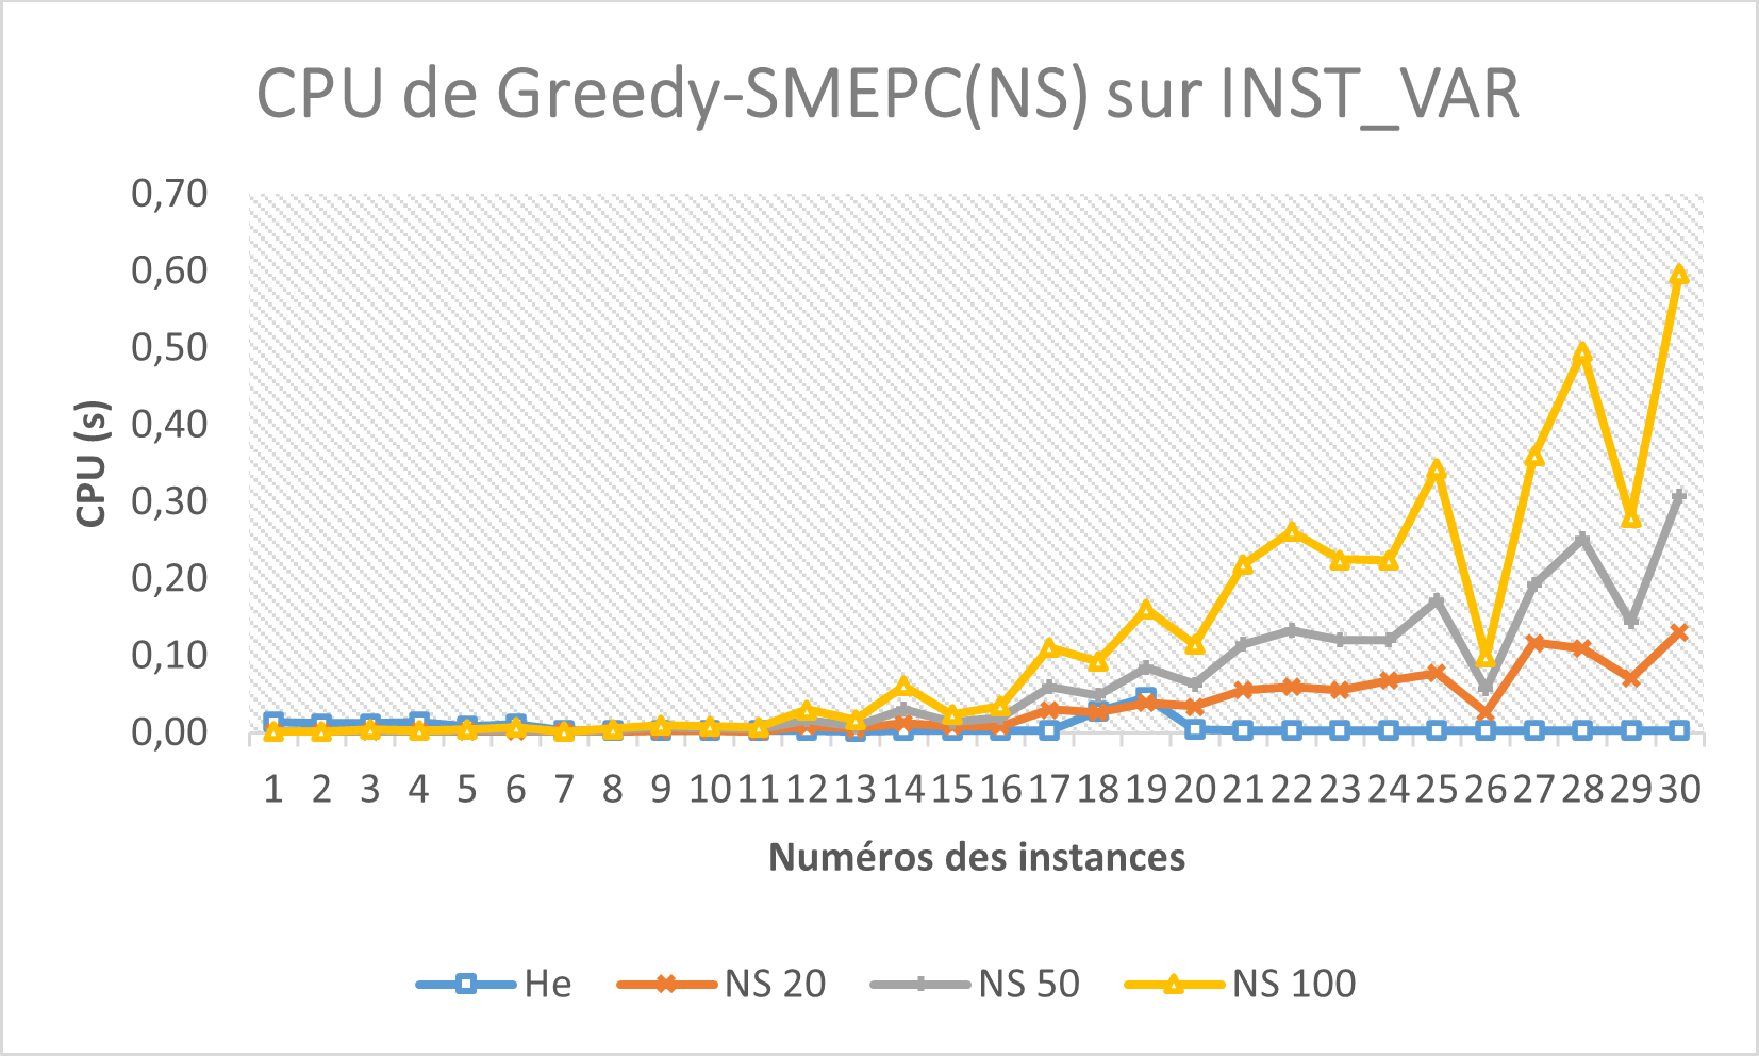
\includegraphics[width=9cm]{images_these/CPU_NS_INST_VAR.pdf}&
		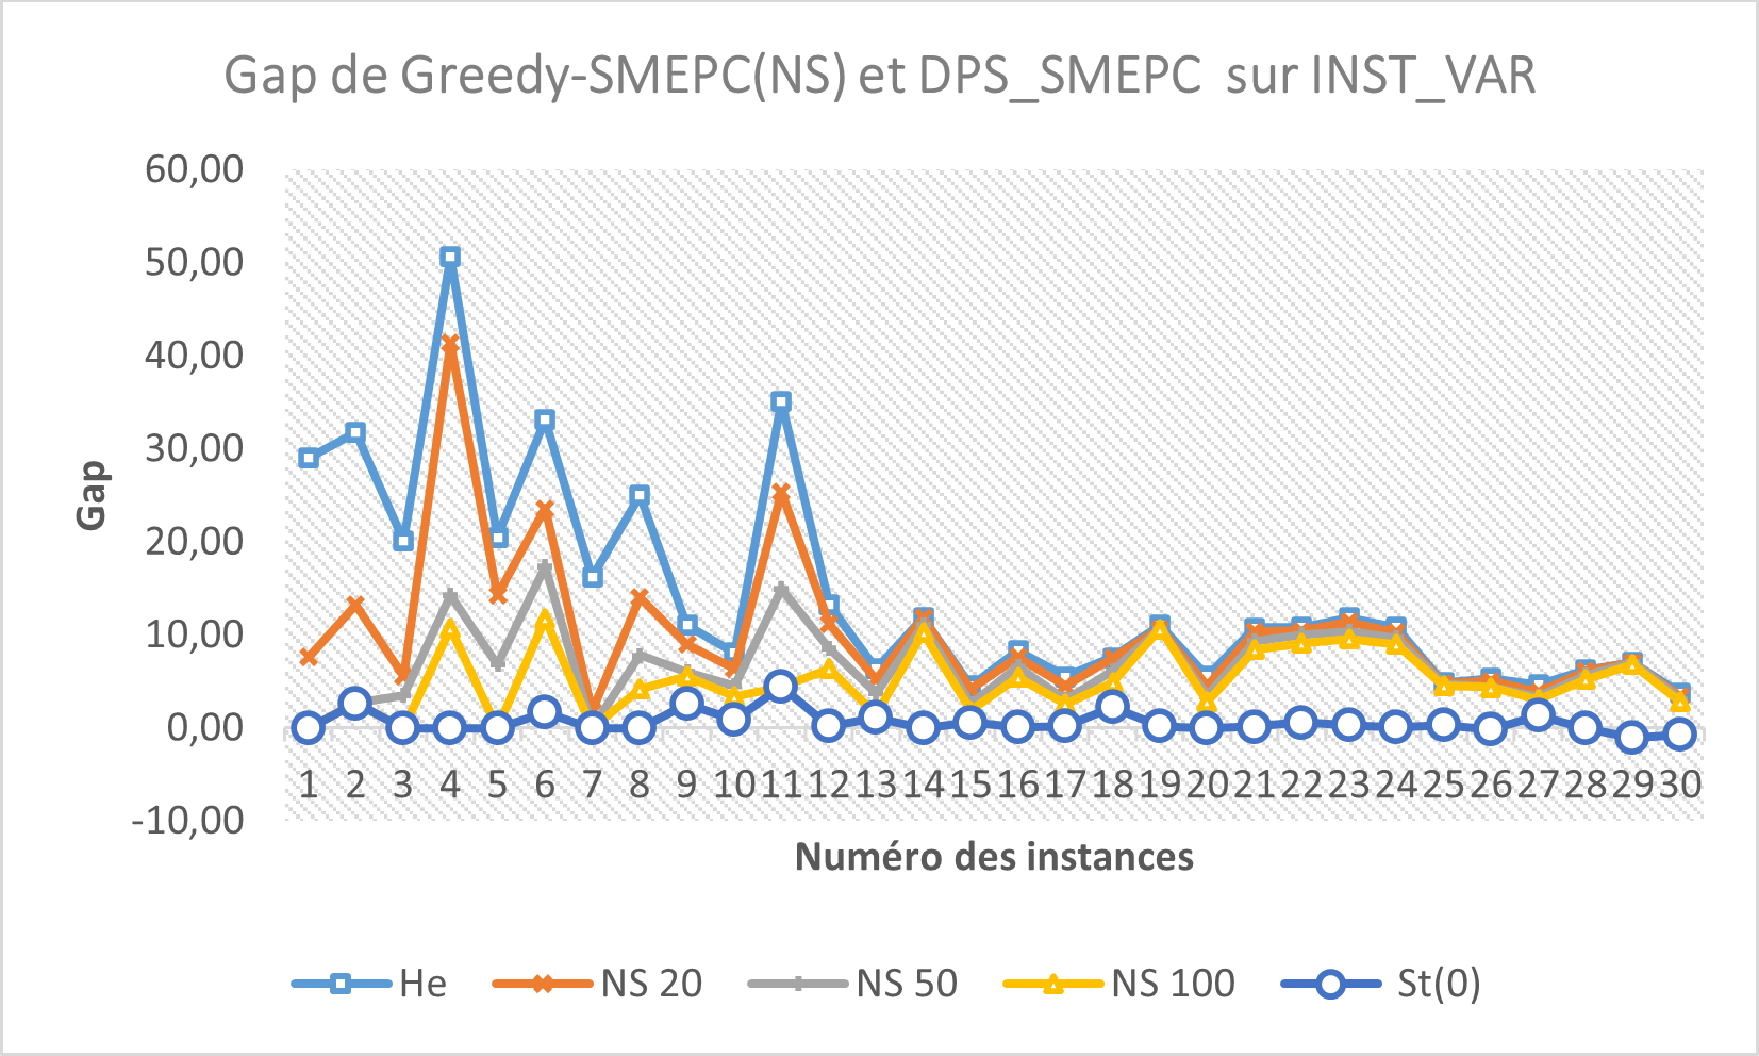
\includegraphics[width=9cm]{images_these/Gap_NS_INST_VAR.pdf}
		\\
		(a) & (b)
	\end{tabular}
	\caption[Représentation graphique du CPU et du gap du tableau (\ref{Comparaison_DPS-SMEPC_greedd})]{Représentation graphique du tableau (\ref{Comparaison_DPS-SMEPC_greedd}) et de $St(0)$. (a) représente le temps CPU et (b) représente le gap à l'optimalité de chaque instance de INST\_VAR.}\label{gap_cpu_NS_INST_VAR}
\end{figure}

\subsubsection{Recherche d'une borne supérieure de qualité pour le DPS\_SMEPC : les instances du paquet INST\_CTE}
 
%On recherche ici la meilleure borne supérieure qu'on utilisera lors de l'exécution de l'algorithme DPS\_SMEPC. Pour cela, on exécute plusieurs algorithmes à la queue leu-leu. Et la borne supérieure sera la meilleure valeur obtenue. La première procédure qu'on exécute est l'heuristique rapide \textbf{He}. En analysant les résultats des instances du paquet INST\_CTE, on remarque que l'algorithme \textbf{He} donne toujours une solution. Cette valeur est utilisée comme borne supérieure de l'algorithme \textbf{Greedy-SMEPC}(20). Lorsqu'un algorithme ne parvient pas à trouver une meilleure solution que sa borne supérieure, on considère que sa valeur est sa borne supérieure.
%La rapidité d'exécution de la procédure \textbf{Greedy-SMEPC}(NS) peut être dû à l'efficacité de l'heuristique rapide \textbf{He}.

%On remarque que lorsqu'on augmente la valeur de $NS$, on obtient de meilleures solutions, ce qui est surement dû au fait que la valeur de la procédure exécutée précédemment est utilisée comme borne supérieure de la procédure suivante.
Consécutivement, le tableau (\ref{Comparaison_DPS-SMEPC_greed2}) présente les résultats des instances du paquet INST\_CTE.
On a plus de la moitié des instances qui ont un gap inférieur à 25\%. 
Le temps d'exécution de tous les algorithmes est toujours inférieur à 0,03 seconde.% En moyenne, la procédure la plus rapide est \textbf{Greedy-SMEPC}(20) et la procédure la plus lente est \textbf{Greedy-SMEPC}(100), ce qui est normal car on garde beaucoup plus d'états. 
%Ici, \textbf{Greedy-SMEPC}(50) est en moyenne plus rapide que l'heuristique \textbf{He}.
%Globalement le gap moyen de \textbf{He}, \textbf{Greedy-SMEPC}(20), \textbf{Greedy-SMEPC}(50), \textbf{Greedy-SMEPC}(100) est respectivement 20,732 ; 14,8525	; 8,5055 ; 5,169 et le temps d'exécution moyen en seconde est respectivement 0,0062 ; 0,0023 ; 0,0049 ; 0,0091. %On constate qu'il y a une amélioration de la valeur  et cela s'accompagne d'une augmentation du temps de calcul, car on augmente le nombre d'états qu'on garde.											


%%%%%%%%%%%%%%%%%%%%%%%%%%%%%%%%%%%%%%%%%%%%%%%%%%%%%%%%%%%%%%%%%%%%%%%%%%%%%%%%%%%%%%%%%
\begin{table}[H]
	\centering
	\small
	\begin{tabular}{|r|rrr|rrr|rrr|rrr|}
		\toprule
		\hline
		\rowcolor{cyan}	& \multicolumn{3}{c|}{\textbf{He}}&\multicolumn{3}{c|}{\textbf{NS(20)}}&\multicolumn{3}{c|}{\textbf{NS(50)}}&\multicolumn{3}{c|}{\textbf{NS(100)}} \\ \hline
		\midrule
		\rowcolor{cyan}	\textbf{num} & \textbf{Obj}& \textbf{Gap}  & \textbf{CPU} & \textbf{Obj}& \textbf{Gap}  & \textbf{CPU} & \textbf{Obj}& \textbf{Gap}  & \textbf{CPU} & \textbf{Obj}&\textbf{Gap}  & \textbf{CPU} \\ \hline
		\midrule
		31	&	325	&	34,85	&	0,02	&	325	&	34,85	&	0,00	&	325	&	34,85	&	0,00	&	325	&	34,85	&	0,00	\\ \hline
		32	&	520	&	45,25	&	0,01	&	520	&	45,25	&	0,00	&	415	&	15,92	&	0,00	&	373	&	4,19	&	0,00	\\ \hline
		33	&	271	&	21,52	&	0,01	&	263	&	17,94	&	0,00	&	231	&	3,59	&	0,00	&	223	&	0,00	&	0,00	\\ \hline
		34	&	259	&	28,22	&	0,01	&	235	&	16,34	&	0,00	&	235	&	16,34	&	0,00	&	235	&	16,34	&	0,00	\\ \hline
		35	&	395	&	53,70	&	0,01	&	323	&	25,68	&	0,00	&	306	&	19,07	&	0,00	&	298	&	15,95	&	0,00	\\ \hline
		36	&	380	&	68,14	&	0,00	&	335	&	48,23	&	0,00	&	276	&	22,12	&	0,00	&	237	&	4,87	&	0,00	\\ \hline
		37	&	222	&	25,42	&	0,01	&	186	&	5,08	&	0,00	&	177	&	0,00	&	0,00	&	177	&	0,00	&	0,00	\\ \hline
		38	&	357	&	26,60	&	0,01	&	303	&	7,45	&	0,00	&	283	&	0,35	&	0,00	&	283	&	0,35	&	0,00	\\ \hline
		39	&	347	&	10,86	&	0,01	&	347	&	10,86	&	0,00	&	341	&	8,95	&	0,00	&	339	&	8,31	&	0,00	\\ \hline
		40	&	361	&	7,44	&	0,01	&	357	&	6,25	&	0,00	&	336	&	0,00	&	0,00	&	336	&	0,00	&	0,00	\\ \hline
		41	&	974	&	8,10	&	0,00	&	945	&	4,88	&	0,00	&	924	&	2,55	&	0,01	&	924	&	2,55	&	0,01	\\ \hline
		42	&	1619	&	12,43	&	0,00	&	1619	&	12,43	&	0,00	&	1593	&	10,63	&	0,01	&	1440	&	0,00	&	0,01	\\ \hline
		43	&	1623	&	5,66	&	0,00	&	1623	&	5,66	&	0,00	&	1623	&	5,66	&	0,01	&	1623	&	5,66	&	0,02	\\ \hline
		44	&	992	&	7,94	&	0,00	&	977	&	6,31	&	0,00	&	960	&	4,46	&	0,01	&	919	&	0,00	&	0,01	\\ \hline
		45	&	957	&	3,01	&	0,00	&	947	&	1,94	&	0,00	&	947	&	1,94	&	0,01	&	947	&	1,94	&	0,01	\\ \hline
		46	&	969	&	13,87	&	0,00	&	945	&	11,05	&	0,00	&	868	&	2,00	&	0,01	&	868	&	2,00	&	0,02	\\ \hline
		47	&	1170	&	24,20	&	0,00	&	1134	&	20,38	&	0,01	&	1016	&	7,86	&	0,01	&	942	&	0,00	&	0,02	\\ \hline
		48	&	1325	&	6,00	&	0,00	&	1325	&	6,00	&	0,01	&	1325	&	6,00	&	0,01	&	1325	&	6,00	&	0,02	\\ \hline
		49	&	886	&	6,62	&	0,00	&	878	&	5,66	&	0,01	&	856	&	3,01	&	0,01	&	831	&	0,00	&	0,02	\\ \hline
		50	&	1132	&	4,81	&	0,00	&	1132	&	4,81	&	0,01	&	1132	&	4,81	&	0,01	&	1084	&	0,37	&	0,02	\\ \hline
		
		\bottomrule
	\end{tabular}%
	\caption{Les instances du paquet INST\_CTE : recherche d'une borne supérieure de qualité pour le DPS\_SMEPC.}
	
	\label{Comparaison_DPS-SMEPC_greed2}%
\end{table}%

\begin{figure}[H]
	\centering
	\begin{tabular}{c c}
		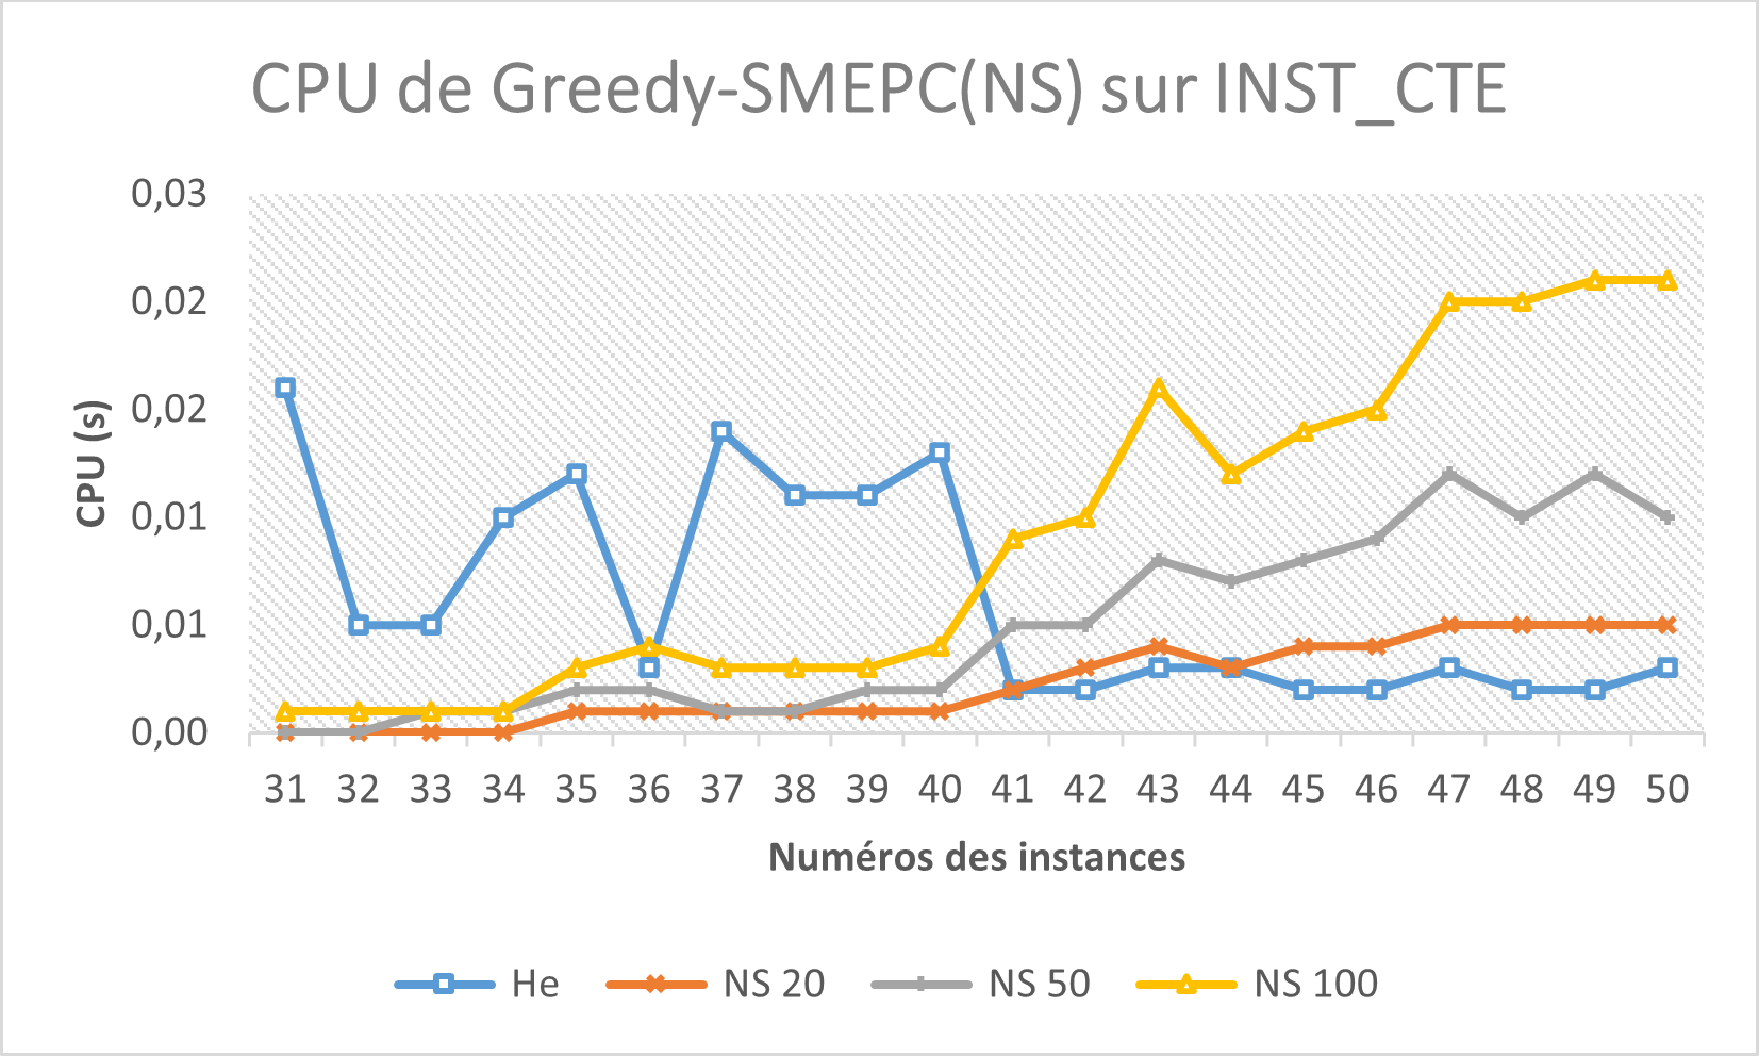
\includegraphics[width=9cm]{images_these/CPU_NS_INST_CTE.pdf}&
		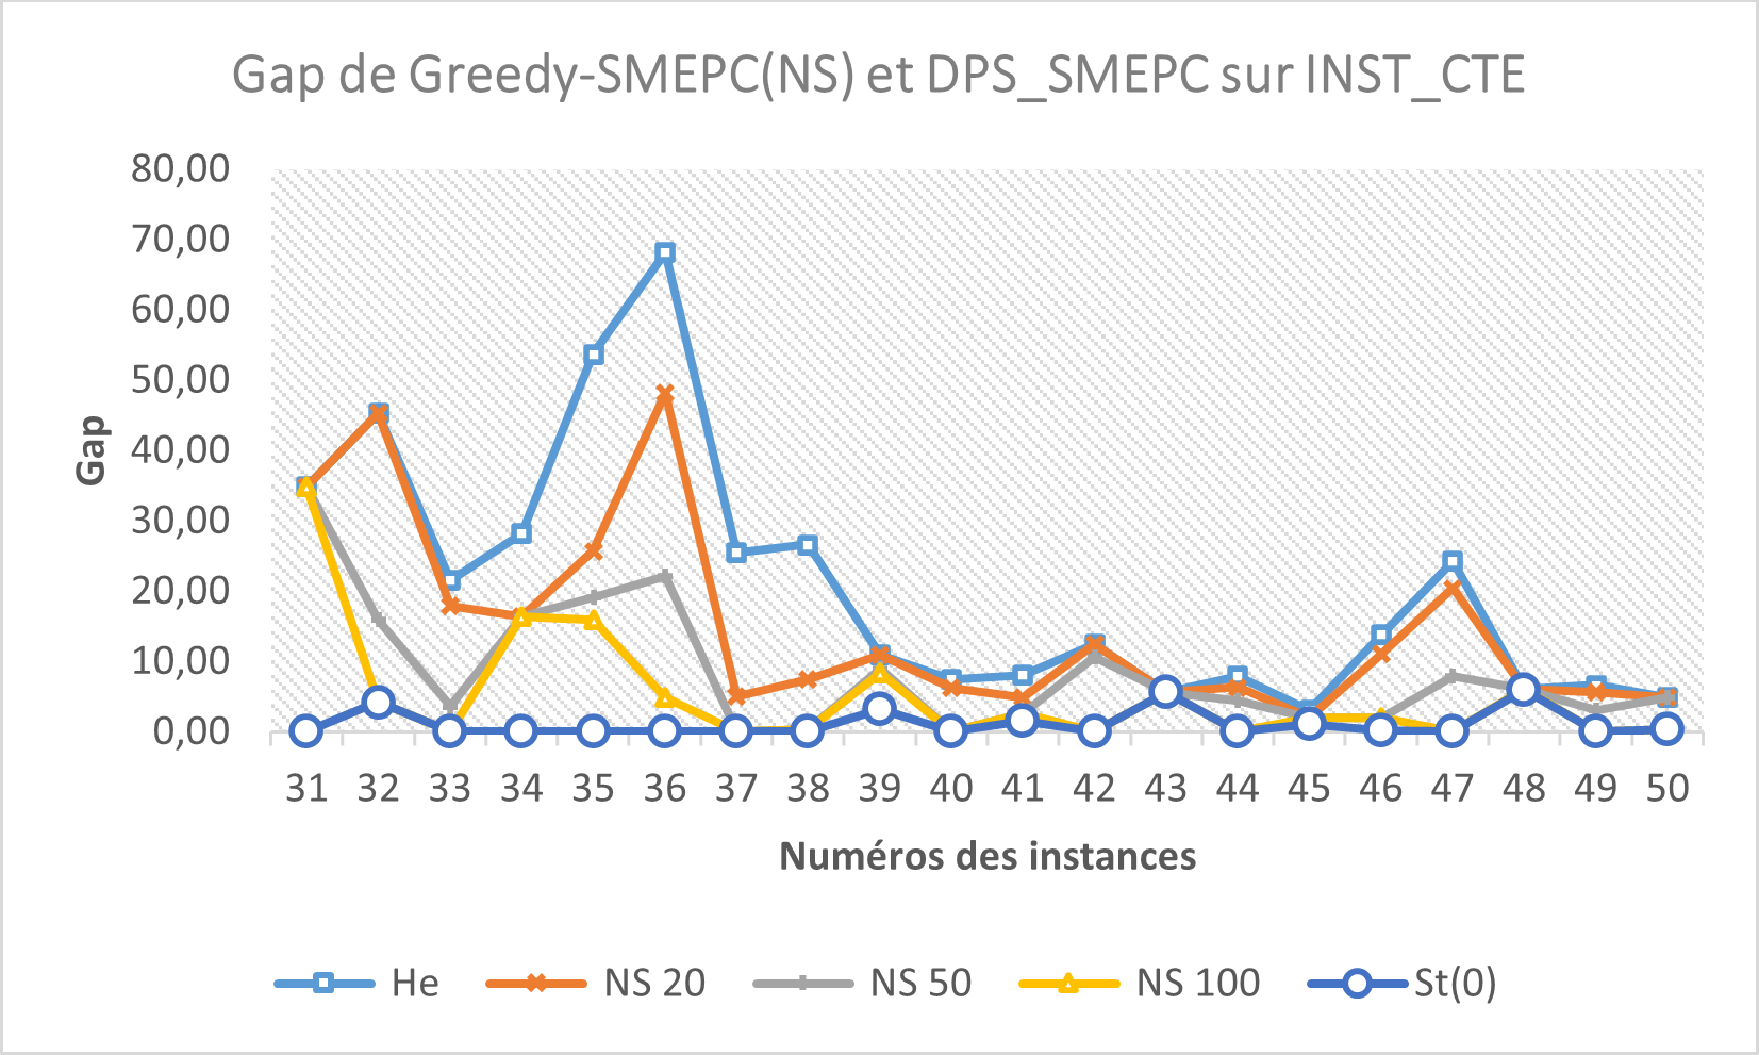
\includegraphics[width=9cm]{images_these/Gap_NS_INST_CTE.pdf}
		\\
		(a) & (b)
	\end{tabular}
	\caption[Représentation graphique du CPU et du gap du tableau (\ref{Comparaison_DPS-SMEPC_greed2})]{Représentation graphique du tableau (\ref{Comparaison_DPS-SMEPC_greed2}) et de $St(0)$. (a) représente le temps CPU et (b) représente le gap à l'optimalité de chaque instance de INST\_CTE.}\label{gap_cpu_NS_INST_CTE}
\end{figure}

On vient de présenter le mécanisme de recherche d'une borne supérieure de qualité pour le DPS\_SMEPC. La section suivante sera consacrée à la mesure de l'impact des mécanismes de filtrage du \textbf{DPS\_SMEPC} sur le nombre d'états générés.

\subsection{Impact des mécanismes de filtrage du DPS\_SMEPC}
%\subsubsection{Résultats}
\label{TempsEnergie}
 Nous voulons obtenir une évaluation de la qualité du schéma de programmation dynamique \textbf{DPS\_SMEPC}. On commence cette partie en rappelant tous les mécanismes de filtrage.
Si on donne maintenant une paire de temps $(i, j)$ et un état connexe $s = (Z, T, V^{Tank}, V^{Veh})$ avec la valeur $W$. Soient $Temps_{j,V^{Veh}}$ et $Energie_{j,V^{Veh}}$ qui représentent respectivement la quantité minimale de temps et d'énergie dont le véhicule  a besoin pour se déplacer de la station $j$ au dépôt final avec la quantité d'hydrogène $V^{Veh}$ dans son réservoir. Afin de limiter le nombre d'états, on applique différents mécanismes de filtrage. En particulier, si on veut ajouter l'état $s$ au temps $(i,j)$, celui-ci doit respecter certains mécanismes de filtrage. Les mécanismes de filtrages qui ont été implémentés sont les suivants :
\begin{enumerate}
	\item Les mécanismes de filtrage logique :
	\begin{itemize} [label=$\square$]
		\item La durée de la tournée ne peut pas être supérieure au temps maximal : $[(i \times p \leq T) \land (T + Temps_{j,V^{Veh}}  \leq TMax)] \lor [(i \times p > T ) \land ( i \times p + d^*_{j+1} + \sum_{j+1\leq k \leq M}t_k \leq TMax)]$
		\item La quantité d'énergie utilisée par le véhicule lors de la tournée ne peut pas être supérieure à la somme de l'énergie stockée et de l'énergie qu'on peut produire : $[(i \times p \leq T ) \land ( V^{Tank} + \sum_{i \leq k \leq N-1}R_k +V^{Veh} \geq Energie_{j,V^{Veh}} )] \lor [(i \times p > T ) \land (V^{Tank} + \sum_{i \leq k \leq N-1}R_k +V^{Veh} \geq \varepsilon^*_{j+1} +\sum_{j+1 \leq k \leq M}e_k )]$
	\end{itemize}
\item Le mécanisme de filtrage par estimation optimiste stipule qu'on supprime un état si ce dernier aboutira à une solution \og moins bonne\fg{} qu'une solution calculée avec une heuristique rapide : 

$W + CostMin(i,Z,(Energie_{j,V^{Veh}}-V^{Tank}-V^{Veh})^+) + \beta \times Temps_{j,V^{Veh}}  \leq BSUP $,

 où $BSUP$ est une borne supérieure calculée avec l'algorithme (\ref{Search_BSUP}). La section précédente était consacré à la présentation du mécanisme de recherche de la valeur $BSUP$.
 
 \item Les mécanismes de filtrage heuristique stipulent que si on trouve dans $(i,j)$ un état $s_1=(Z_1, T_1, V^{Tank}_1, V^{Veh}_1)$ (accompagné d'une valeur $W_1$) qui est équivalent modulo $K$ à $s$ alors si $W<W_1$ alors on remplace $E_1$, $W_1$ par $E$, $W$ dans les états du temps $(i,j)$. Les états $s$ et $s_1$ sont équivalents modulo $K$ si $Z =Z_1$ et $|V^{Tank} - V^{Tank}_1| \leq (C^{Tank} / K)$ et $|V^{Veh} - V^{Veh}_1| \leq (C^{Veh} / K)$ et $|T - T_1| \leq (\Pi_j / K)$. sachant que le paramètre $K$ doit être préalablement préfixé.
\end{enumerate}

Nous voulons ici obtenir une évaluation de l'impact des mécanismes de filtrage décrit ci-dessus. Cet impact est à double sens : premièrement, il fait diminuer le nombre d'états qui sont traités tout au long du processus ; deuxièmement, le filtrage heuristique peut induire un gap entre la solution obtenue et la solution optimale.
 On exécute \textbf{DPS\_SMEPC} de quatre manières : 
\begin{enumerate}
	
	\item Sans mécanismes de filtrage, on nomme ces résultats $St(1)$ ;
	\item Avec les mécanismes de filtrage logique, on nomme ces résultats $St(2)$ ;
	\item Avec les mécanismes de filtrage logique et les mécanismes de filtrage par estimation optimiste, on nomme ces résultats $St(3)$ ;
	\item Avec les mécanismes de filtrage logique, les mécanismes de filtrage par estimation optimiste et les mécanismes de filtrage heuristique, on nomme ces résultats $St(0)$. Concernant le filtrage heuristique, on a testé plusieurs valeurs de $K$ et on a choisi la plus petite valeur qui permettait d'avoir une solution de chaque instance. Le paramètre obtenu pour ces instances est $K=7$.
	
\end{enumerate}


%Nous nous concentrons sur les nombres maximaux \# Etats Max, \# Etats LOG et \# Etats (BSUP NS 50) d'états $s$ qui sont gérés pour une paire donnée $(i, j)$. 
%$\#etats max$ est le nombre d'état obtenus au maximum sans mécanismes de filtrage. $ST\_Gap(i)$ est le gap entre la solution obtenue et la solution optimale en exécutant \textbf{DPS\_SMEPC} avec uniquement la mécanisme de filtrage $ST(i)$. Ceci est fait pour mesurer si l'application ou non des mécanismes de filtrage ont un impact sur la solution optimale.
%\begin{landscape}
%(\ref{power_filter})
\poubelle{
\begin{center}
	\tablefirsthead{%
	\rowcolor{cyan}	\hline\multicolumn{1}{|c|}{\tbsp Instance
			Id: (N, M, p)}  &\# Etats Max  &  \# Etats LOG &\# Etats (BSUP NS 50) \\\hline}
	\tablehead{%
	\rowcolor{cyan}	\hline\multicolumn{4}{|c|}{\small\sl suite de la page précédente }\\
	\rowcolor{cyan}\hline\multicolumn{1}{|c|}{\tbsp Instance
			Id: (N, M, p)} &\# Etats Max  &  \# Etats LOG &\# Etats (BSUP NS 50) \\\hline}
	\tabletail{%
	\rowcolor{cyan}	\hline\multicolumn{4}{|c|}{\small\sl suite à la page suivante}\\\hline}\tablelasttail{\hline}\bottomcaption{Pouvoir de filtrage des mécanismes de filtrage logiques et basées sur la qualité.\label{power_filter}}
	\small
	\begin{supertabular}{|*{4}{c|}}
		%\hline
		1 : (15, 4, 4)&	576000&	421&	28\\
		\hline
		2 : (78, 10, 1)&	1137240	&31810&	30873\\
		\hline
		3 : (94, 10, 1)&	1086640&	22394&	20370\\
		\hline
		4 : (114, 10, 1)&	1206120&	40032&	9030\\
		\hline
		5 : (99, 10, 1)	&714780&	32765&	10281\\
		\hline
		6 : (59, 10, 2)&	1142240	&53053&	13339\\
		\hline
		7 : (36, 10, 2)&	1559520&	28876&	3082\\
		\hline
		8 : (78, 10, 2)&	1510080&	81790&	10536\\
		\hline
		9 : (57, 10, 2)&	1206120&	16028&	2938\\
		\hline
		10 : (26, 8, 4)	&718848&	13476&	916\\
		\hline
		11 : (26, 10, 4)&	936000&	8060&	2844\\
		\hline
		12 : (24, 10, 4)&	300000&	4800&	1933\\
		\hline
		13 : (30, 10, 4)&	173400&	14929&	7916\\
		\hline
		14 : (33, 8, 4)&	356928&	18761&	12201\\
		\hline
		15 : (20, 8, 4)&	576000&	8078&	581\\
		\hline
		16 : (25, 8, 4)&	705600&	16658&	3503\\
		\hline
		17 : (27, 8, 4)&	876096&	48501&	312\\
		\hline
		18 : (50, 10, 4)&	3136000	&118795&	10608\\
		\hline
		19 : (24, 10, 4)&	3317760&	31415&	7995\\
		\hline
		20 : (44, 10, 4)&	2816000	&26639&	492\\
		\hline
		21 : (32, 12, 4)&	602112&	11589&	10805\\
		\hline
		22 : (32, 12, 4)&	602112	&11589&	10805\\
		\hline
		23 : (45, 14, 4)&	2903040&	28073&	22307\\
		\hline
		24 : (30, 8, 4)	&1614720&	13608&	11486\\
		\hline
		25 : (26, 8, 4)	&2416128&	10989&	2730\\
		\hline
		26 : (17, 10, 4)&	199920&	6013&	35\\
		\hline
		27 : (19, 10, 4)&	291840&	887	&370\\
		\hline
		28 : (20, 10, 4)&	291600&	1718&	545\\
		\hline
		29 : (50, 12, 4)&	3110400&41858&	25020\\
		\hline
		30 : (50, 12, 4)&	3110400	&40820&	25020\\
		
	\end{supertabular}
\end{center}
}
%\begin{table}[htbp]
%	\begin{center}
%		\begin{tabular}{|*{9}{c|}}
%			\hline
%			$(M,N)$ & $\#etats max$ & $\# Etats Max$ & $\# Etats LOG$  & $State\_DPS\_SMEPC$& $ST\_Gap(1)$ & $ST\_Gap(2)$  & $ST\_Gap(3)$ \\
%			\hline
%		\end{tabular}
%		\caption{Impact des mécanismes de filtrage sur le DPS\_SMEPC. \label{mécanismes_filtrage}}
%	\end{center}
%\end{table}
%\end{landscape}
%# Etats (BSUP NS 50) ==Etats DPS global(BSUP NS 50)
%$\#$ Etats ($X$) est le nombre d'états du DPS global avec comme borne supérieure la borne supérieure BSUP qui représente la valeur de la procédure $X$.
%BSUP pipe représente la procédure décrite au chapitre suivant et BSUP PL 1 sec représente $MILP_{SMEPC}$ lorsqu'on impose comme temps d'exécution maximale 1 seconde.

\poubelle{
\begin{center}
	\tablefirsthead{%
	\rowcolor{cyan}	\hline\multicolumn{1}{|c|}{\tbsp Instance
			Id: (N, M, p)}  &\# Etats (BSUP NS 50)  &\# Etats (BSUP pipe) & \# Etats (BSUP PL 1 sec)\\\hline}
	\tablehead{%
	\rowcolor{cyan}	\hline\multicolumn{4}{|c|}{\small\sl suite de la page précédente }\\
	\rowcolor{cyan}\hline\multicolumn{1}{|c|}{\tbsp Instance
				Id: (N, M, p)}  &\# Etats (BSUP NS 50)  &\# Etats (BSUP pipe) & \# Etats (BSUP PL 1 sec)\\\hline}
	\tabletail{%
	\rowcolor{cyan}	\hline\multicolumn{4}{|c|}{\small\sl suite à la page suivante}\\\hline}\tablelasttail{\hline}\bottomcaption{Pouvoir de filtrage des mécanismes de filtrage logiques et basées sur la qualité (en fonction de la BSUP utilisée).\label{power_filter2}}
	\small
	\begin{supertabular}{|*{4}{c|}}
		\hline
1 : (15, 4, 4)& 28&	36&	28\\
\hline
2 : (78, 10, 1)& 30873&	4146&	9303\\
\hline
3 : (94, 10, 1)& 20370&		1122&	1639\\
\hline
4 : (114, 10, 1)& 9030&	4209&	14014\\
\hline
5 : (99, 10, 1)	&10281&	6848&	29761\\
\hline
6 : (59, 10, 2)& 13339&	10197&	10964\\
\hline
7 : (36, 10, 2)& 3082&		93&	61\\
\hline
8 : (78, 10, 2)& 10536&	9727&	21442\\
\hline
9 : (57, 10, 2)& 2938&	1988&	3687\\
\hline
10 : (26, 8, 4)	& 916&	916&	1564\\
\hline
11 : (26, 10, 4)& 2844&	123&	344\\
\hline
12 : (24, 10, 4)& 1933&		1891&	1741\\
\hline
13 : (30, 10, 4)& 7916&	7763&	7583\\
\hline
14 : (33, 8, 4)& 12201&	3796&	9775\\
\hline
15 : (20, 8, 4)& 581&	335&	246\\
\hline
16 : (25, 8, 4)& 3503&	16439&	7654\\
\hline
17 : (27, 8, 4)& 312&	410	&312\\
\hline
18 : (50, 10, 4)& 10608&	4360&	12533\\
\hline
19 : (24, 10, 4)& 7995&	65&	222\\
\hline
20 : (44, 10, 4)& 492&	104&	104\\
\hline
21 : (32, 12, 4)& 10805&	10189&	10404\\
\hline
22 : (32, 12, 4)& 10805&	10189&	10579\\
\hline
23 : (45, 14, 4)& 22307&	16700&	16334\\
\hline
24 : (30, 8, 4)	& 11486&	3014&	8608\\
\hline
25 : (26, 8, 4)	& 2730&	121&	121\\
\hline
26 : (17, 10, 4)& 35&	35&	35\\
\hline
27 : (19, 10, 4)& 370&	101&	403\\
\hline
28 : (20, 10, 4)& 545&	558&	16629\\
\hline
29 : (50, 12, 4)& 25020&	1966&	41858\\
\hline
30 : (50, 12, 4)& 25020&	1966&	41858\\

	\end{supertabular}
\end{center}
}
%	\subsubsection{Interprétations}

Les tableaux (\ref{power_filter}) et (\ref{power_filter2}) présentent les résultats de $St(0)$, $St(1)$, $St(2)$ et $St(3)$ respectivement pour les instances du paquet INST\_CTE et du paquet INST\_VAR. La signification des colonnes est :
\begin{itemize}[label=$\square$]
	\item  \textbf{Obj} est la valeur obtenue ;
	\item \textbf{Gap} est le gap par rapport à l'optimalité $Gap  = 100 \times \frac{Obj-opt}{opt}$ ; où $Obj$ est la valeur obtenue et $opt$ est la valeur optimale obtenue à l'aide du modèle $MILP_{SMEPC}$ du chapitre précédent. Si une instance n'a pas été résolu jusqu'à l'optimalité, on utilise la borne supérieure du modèle exécuté sur CPLEX sur 8 threads avec un temps limite de 3 heures (voir tableau (\ref{tab:resultSYM_STC}) et (\ref{tab:resultSYM_STC2})).
	\item \textbf{\#Etats} est le nombre d'états maximal générés
	\item \textbf{CPU} est le temps d'exécution. 
\end{itemize}

%On cherche à obtenir une évaluation de l'impact des mécanismes de filtrage. Pour cela, 
On exécute plusieurs fois l'algorithme \textbf{DPS\_SMEPC} en activant à chaque fois les filtrages qui nous intéressent. La borne supérieure a été calculée par l'algorithme (\ref{Search_BSUP}). On n'a pas inscrit dans le tableau les valeurs objectives de $St(2)$ et $St(1)$ car elles sont identiques à la valeur de $St(3)$. On ne calcule pas le gap de $St(1)$, $St(2)$ et $St(3)$ car on obtient la valeur optimale donc le gap vaut zéro.

On remarque que lorsqu'on ajoute des mécanismes de filtrage l'algorithme est de plus en plus rapide car les mécanismes de filtrage diminuent le nombre d'états. En comparant le nombre d'états $\#Etats$ des algorithmes, on remarque que le mécanisme de filtrage exact le plus efficace est le filtrage par estimation optimiste. 

On fait les remarques suivantes :
\begin{itemize}[label=$\square$]
	
	\item L'ajout du filtrage heuristique ($ST(0)$) permet d'obtenir une solution à toutes les instances et ces solutions sont proches (inférieure à 6\%) de celles obtenues par CPLEX (3 heures et 8 threads). Pour 5 instances du paquet INST\_VAR on obtient de meilleures solutions que la borne supérieure calculée par CPLEX ;
	\item On constate que le temps CPU de la colonne $ST(0)$ est très faible comparé aux résultats de CPLEX. De plus l'algorithme devient plus rapide avec le filtrage heuristique qu'avec uniquement les filtrages exactes ;
	\item  C'est uniquement sur le paquet d'instances INST\_VAR qu'on voit une diminution du gap lors de l'ajout du filtrage heuristique. On résout des instances qu'on ne résolvait pas avec les filtrages exactes. 
	\item Toutes les instances du paquet INST\_CTE sont résolues jusqu'à l'optimum avec les filtrages exactes. Or, ce n'est pas le cas pour le paquet d'instances INST\_VAR. En effet, on n'arrive pas à résoudre 17 instances du paquet INST\_VAR lorsqu'on utilise uniquement les filtrages exactes ;
	\item Les solutions obtenues par $ST(0)$ sont meilleures que les valeurs des heuristiques de la section précédente. Ceci est dû au fait que la meilleure valeur calculée par les heuristiques est utilisée comme borne supérieure lors du filtrage par estimation optimiste ;
	\item Le nombre d'états obtenus par le paquet d'instances INST\_VAR est supérieur au nombre d'états du paquet d'instances INST\_CTE. On fait la même remarque pour le temps de calcul.
	
\end{itemize}
\subsubsection{Impact des mécanismes de filtrage du DPS\_SMEPC : les instances du paquet INST\_VAR}
\label{B_power_filter2}
Le tableau (\ref{power_filter}) présente les résultats des instances du paquet INST\_VAR.
%On cherche à obtenir une évaluation de l'impact des mécanismes de filtrage. Pour cela, on exécute plusieurs fois l'algorithme \textbf{DPS\_SMEPC} en activant à chaque fois les filtrages qui nous intéressent. La borne supérieure est celle obtenue à la section précédente. On n'a pas inscrit dans le tableau les valeurs objectifs de $St(2)$ et $St(1)$ car elles sont identiques à la valeur de $St(3)$. On ne calcule pas le gap de $St(1)$, $St(2)$ et $St(3)$ car on obtient la valeur optimale donc le gap vaut zéro.
 Lorsque la valeur vaut \og - \fg{} cela veut dire que l'algorithme s'est arrêté au bout d'une heure sans trouver de solution.
Le gap moyen de $St(0)$ est 0,596\%.
En analysant les résultats des instances du paquet INST\_VAR, on remarque que le filtrage heuristique est efficace car on obtient toujours une solution de bonne qualité en moins d'une heure. Or, en ajoutant les filtrages exactes au DPS\_SMEPC ($St(1)$, $St(2)$ et $St(3)$), on ne parvient pas à résoudre 56,6\% des instances en moins d'une heure. De plus, en ajoutant le filtrage heuristique la méthode devient très rapide et on obtient des gaps qui sont inférieurs à 5\%, ces filtrages ne dégradent que légèrement la solution. De plus avec le filtrage heuristique on obtient 6 solutions optimales en moins de 0,02 seconde. Par exemple, pour l'instance 16, on passe de 1,02 heure de temps d'exécution lorsqu'on exécute sans filtrage à 0,037 seconde lorsqu'on exécute avec tous les filtrages et on a un gap de 0,08\%. 
Globalement le nombre d'états moyen des colonnes $St(0)$, $St(3)$, $St(2)$, $St(1)$ est respectivement 2449,133 ; 799762,7333 ; 962697,333 ; 1033360,2
et le temps d'exécution moyen en minutes est respectivement 0,96 ; 36,1048 ; 44,11 ; 44,75. 
%On remarque que lorsqu'on ajoute des mécanismes de filtrage l'algorithme est de plus en plus rapide car les mécanismes de filtrage diminuent le nombre d'états. En comparant le nombre d'états de chaque algorithme, on constante que le mécanisme de filtrage exact le plus efficace est le filtrage par estimation optimiste.

%%%%%%%%%%%%%%%%%%%%%%%%%%%%%%%%%%%%%%%%%%%%%%%%%%%%%%%%%%%%%%%%%%%%%%%%%%%%%%%%%%%%%%%%%
\begin{table}[H]
	\centering
	\small
	\begin{tabular}{|r|rrrr|rrr|rr|rr|}
		\toprule
		\hline
		\rowcolor{cyan}	&\multicolumn{4}{c|}{\textbf{St(0)}} & \multicolumn{3}{c|}{\textbf{St(3)}}&\multicolumn{2}{c|}{\textbf{St(2)}}&\multicolumn{2}{c|}{\textbf{St(1)}} \\ \hline
		\midrule
		
		\hline
		\rowcolor{cyan}	&\multicolumn{4}{c|}{ \tiny{Tous les filtrages exacts et heuristiques}} & \multicolumn{3}{c|}{\tiny{Tous les filtrages exacts}}&\multicolumn{2}{c|}{\tiny{Filtrages logiques et optimistes}}&\multicolumn{2}{c|}{\tiny{Sans filtrage}}
		\\ \hline
		\midrule
		
		\rowcolor{cyan}	\textbf{num} &\textbf{Obj} & \textbf{Gap} & \textbf{\#Etats} & \textbf{CPU} &\textbf{Obj} & \textbf{\#Etats} & \textbf{CPU}  & \textbf{\#Etats} & \textbf{CPU}  & \textbf{\#Etats} & \textbf{CPU} \\ \hline
		\midrule
	1	&	131	&	0,00	&	61	&	0,00	&	131	&	554	&	0,00	&	4329	&	0,02	&	4604	&	0,03	\\ \hline
	2	&	155	&	2,65	&	161	&	0,00	&	151	&	1739	&	0,01	&	4241	&	0,04	&	4820	&	0,04	\\ \hline
	3	&	144	&	0,00	&	63	&	0,00	&	144	&	2213	&	0,03	&	129720	&	15,38	&	131744	&	15,91	\\ \hline
	4	&	140	&	0,00	&	321	&	0,01	&	140	&	2155	&	0,03	&	4748	&	0,06	&	4865	&	0,07	\\ \hline
	5	&	161	&	0,00	&	48	&	0,00	&	161	&	406	&	0,01	&	82005	&	9,62	&	83001	&	9,75	\\ \hline
	6	&	181	&	1,69	&	198	&	0,01	&	178	&	9960	&	0,26	&	13761	&	0,65	&	19072	&	0,84	\\ \hline
	7	&	222	&	0,00	&	126	&	0,00	&	222	&	1732	&	0,01	&	7914	&	0,07	&	14375	&	0,17	\\ \hline
	8	&	192	&	0,00	&	87	&	0,00	&	192	&	1607	&	0,02	&	37060	&	4,23	&	39376	&	4,44	\\ \hline
	9	&	661	&	2,64	&	286	&	0,04	&	644	&	263867	&	329,67	&	1410815	&	3910,25	&	1344462	&	4321,23	\\ \hline
	10	&	1149	&	0,88	&	148	&	0,02	&	1139	&	326094	&	127,00	&	716815	&	3810,17	&	1024128	&	3676,93	\\ \hline
	11	&	140	&	4,48	&	29	&	0,00	&	134	&	536	&	0,01	&	42913	&	6,75	&	43867	&	6,98	\\ \hline
	12	&	914	&	0,22	&	314	&	0,14	&	-	&	613249	&	3613,47	&	1020778	&	3856,31	&	1020778	&	3707,92	\\ \hline
	13	&	967	&	1,15	&	59	&	0,01	&	956	&	7115	&	0,70	&	1610932	&	3673,96	&	1610932	&	3844,40	\\ \hline
	14	&	1372	&	0,00	&	642	&	0,63	&	-	&	1550626	&	3602,32	&	1559487	&	3710,34	&	1559487	&	3862,77	\\ \hline
	15	&	1354	&	0,59	&	106	&	0,03	&	1346	&	261078	&	408,83	&	1067321	&	3799,09	&	1115578	&	4056,97	\\ \hline
	16	&	1292	&	0,08	&	429	&	0,37	&	-	&	909386	&	4080,64	&	1118045	&	3751,39	&	1118045	&	3684,39	\\ \hline
	17	&	1288	&	0,23	&	410	&	0,71	&	-	&	703595	&	3809,08	&	1019333	&	3769,64	&	1169832	&	3678,05	\\ \hline
	18	&	2427	&	2,28	&	390	&	0,44	&	-	&	872810	&	3701,67	&	764772	&	3664,77	&	1256433	&	3631,32	\\ \hline
	19	&	2218	&	0,23	&	442	&	1,94	&	-	&	2238483	&	3642,79	&	2010204	&	3654,53	&	2238483	&	3660,75	\\ \hline
	20	&	2657	&	-0,08	&	609	&	1,43	&	-	&	1137757	&	3646,60	&	918477	&	3839,88	&	1227651	&	3759,62	\\ \hline
	21	&	1412	&	0,14	&	2138	&	10,98	&	-	&	1207299	&	3671,79	&	846485	&	3611,51	&	1219554	&	3631,16	\\ \hline
	22	&	1350	&	0,60	&	5148	&	38,67	&	-	&	1759894	&	4088,15	&	1687911	&	3630,61	&	1850181	&	4065,63	\\ \hline
	23	&	2598	&	0,31	&	1284	&	4,92	&	-	&	1320005	&	3694,15	&	1320005	&	3672,38	&	1320005	&	3660,03	\\ \hline
	24	&	2808	&	0,11	&	1116	&	5,18	&	-	&	1450961	&	3738,81	&	1450961	&	3626,02	&	1450961	&	3660,26	\\ \hline
	25	&	2060	&	0,34	&	869	&	7,89	&	-	&	1626287	&	3715,09	&	1484155	&	3660,78	&	1484155	&	3639,51	\\ \hline
	26	&	2353	&	-0,13	&	53759	&	1604,02	&	-	&	1550660	&	3638,91	&	1637832	&	3642,65	&	1637832	&	3782,43	\\ \hline
	27	&	2500	&	1,30	&	696	&	4,26	&	-	&	1817157	&	3624,48	&	2510242	&	4460,81	&	2510242	&	4507,72	\\ \hline
	28	&	3053	&	-0,03	&	1258	&	11,85	&	-	&	1468315	&	3853,50	&	1468854	&	3727,84	&	1468854	&	4227,10	\\ \hline
	29	&	4390	&	-1,06	&	1070	&	8,65	&	-	&	1764386	&	4155,38	&	1764386	&	4127,95	&	1861070	&	3726,37	\\ \hline
	30	&	3496	&	-0,74	&	1207	&	17,69	&	-	&	1122956	&	3845,23	&	1166419	&	3758,72	&	1166419	&	3723,97	\\ \hline
		\bottomrule
	\end{tabular}%
	\caption{Les instances du paquet INST\_VAR : impact des mécanismes de filtrage du DPS\_SMEPC.}
	\label{power_filter}%
\end{table}%

\begin{figure}[H]
	\centering
	\begin{tabular}{c c}
		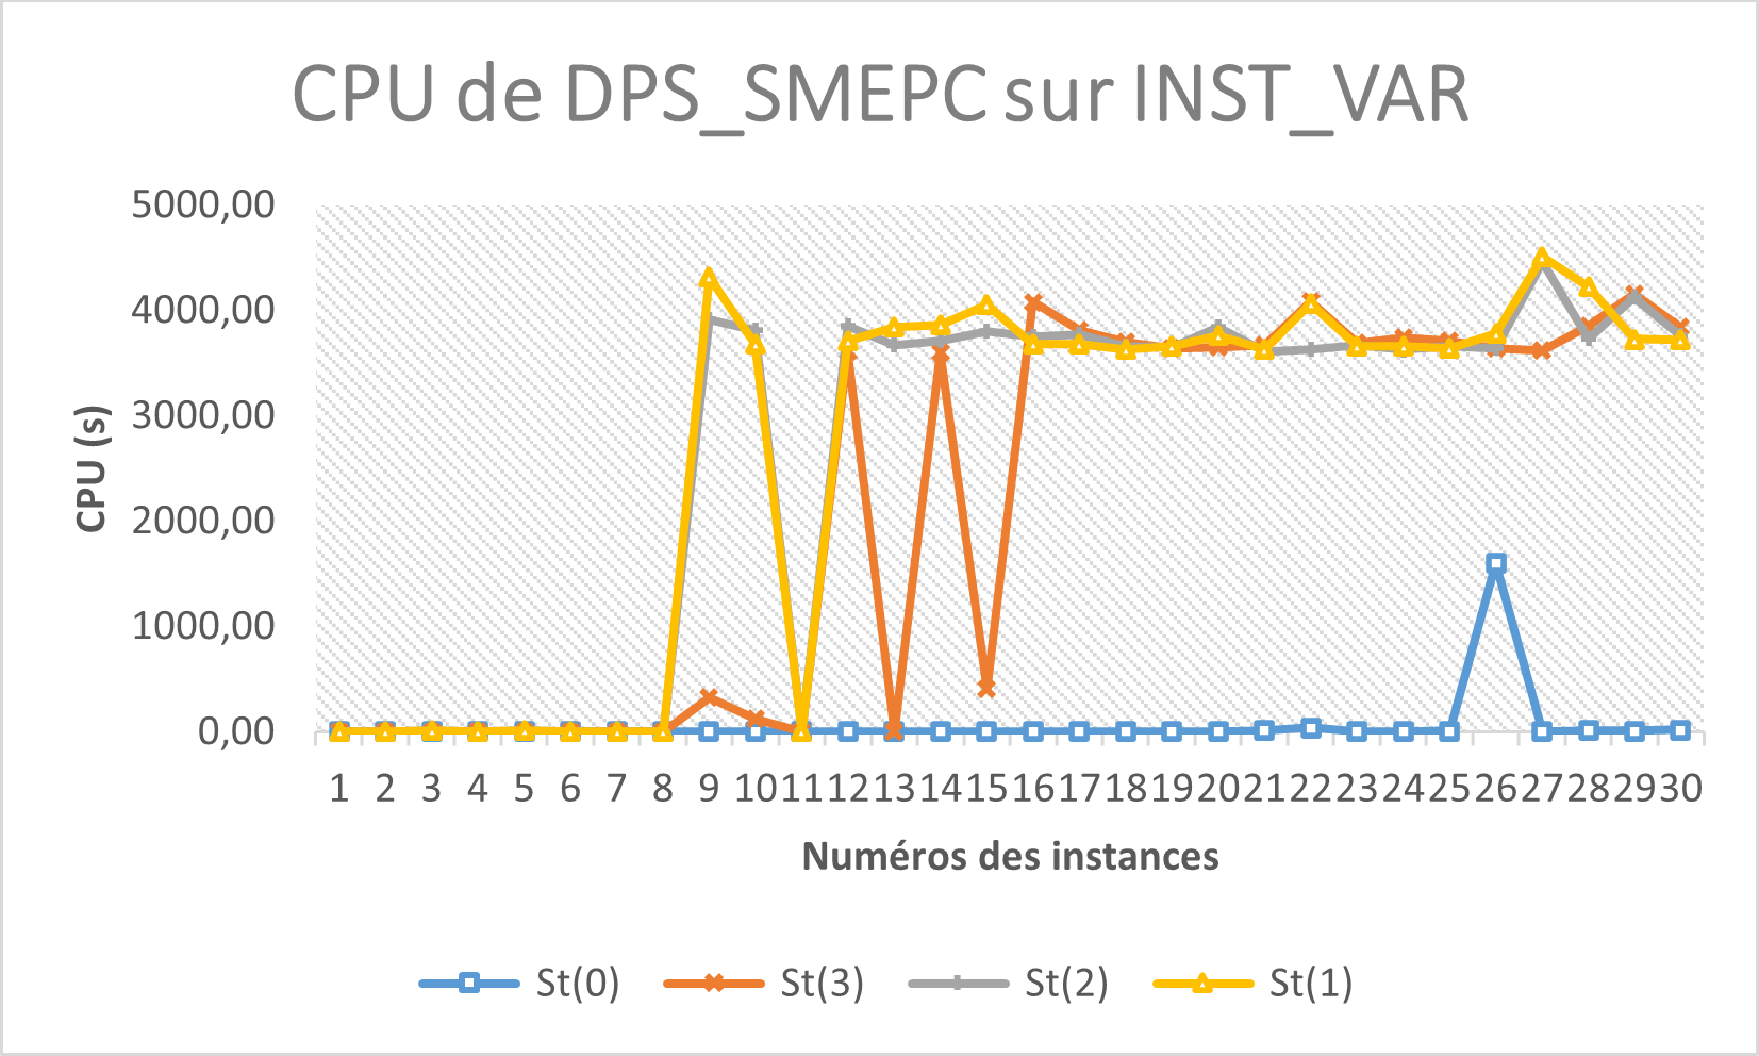
\includegraphics[width=9cm]{images_these/CPU_DPS_SMEPC_INST_VAR.pdf}&
		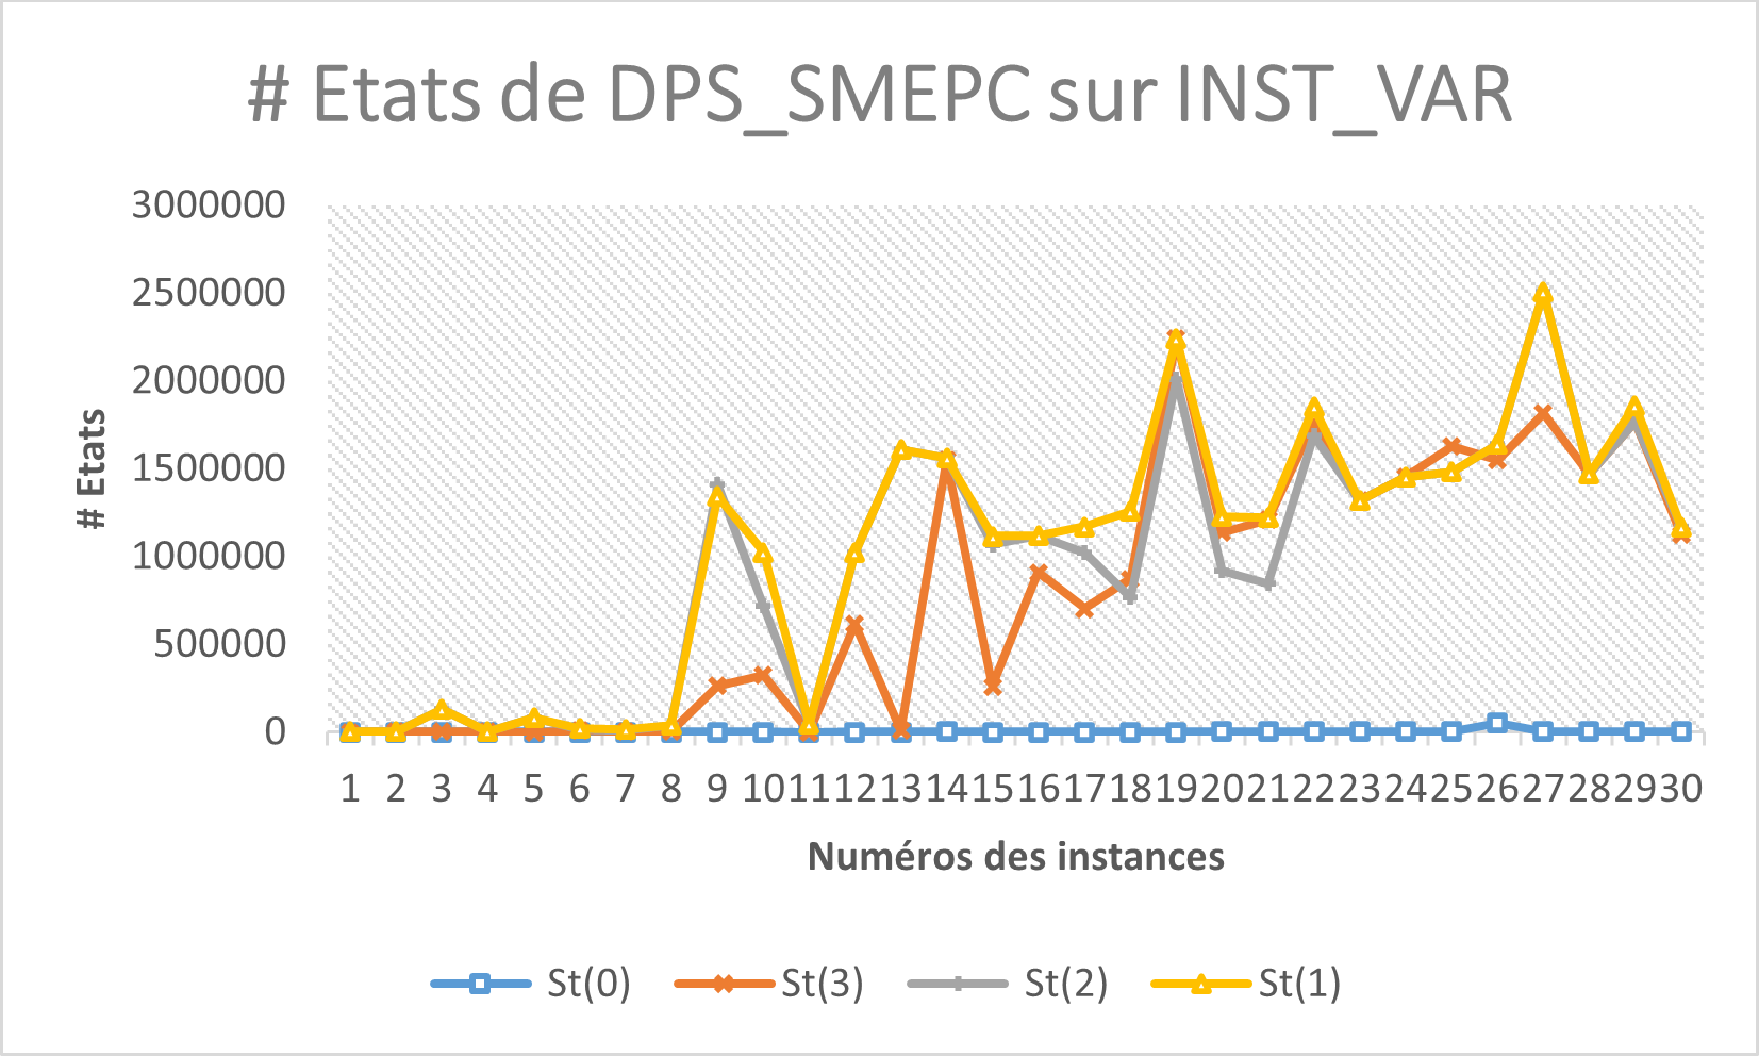
\includegraphics[width=9cm]{images_these/Etats_DPS_SMEPC_INST_VAR.pdf}
		\\
		(a) & (b)
	\end{tabular}
	\caption[Représentation graphique du CPU et du gap du tableau (\ref{power_filter})]{Représentation graphique du tableau (\ref{power_filter}). (a) représente le temps CPU et (b) représente le nombre d'états de chaque instance de INST\_VAR.}\label{gap_cpu_dps_smepc_INST_VAR}
\end{figure}

%On vient de mesurer l'impact des mécanismes de filtrage du \textbf{DPS\_SMEPC} sur le nombre d'états générés. La section suivante sera consacrée aux expérimentations numériques du Greedy-DPS et du \textbf{DPS\_SMEPC}.



%\begin{table}[htbp]
%	\begin{center}
%		\begin{tabular}{|*{5}{c|}}
%			\hline
			%(N,M)  & Coût DPS\_SMEPC  &Coût Greedy-SMEPC &Coût NS 10&Coût NS 50&Coût NS 100 \\
%			$(M,N)$  & $G\_Gap$ &$W\_Gap(100)$ & $W\_Gap(50)$&   $W\_Gap(10)$\\
%			\hline
			
%		\end{tabular}
%		\caption{Comparaison du DPS\_SMEPC et du Greedy-SMEPC . \label{ Gap1}}
%	\end{center}
%\end{table}


% Résultats : Nous fixons ici CVeh = 20, et CMP = 50, TMax = 200, et faisons varier N, M et NS. Nous obtenons alors, pour tout ensemble de 5 exemples, les valeurs moyennes suivantes :  
%	\subsubsection{Interprétations}
\subsubsection{Impact des mécanismes de filtrage du DPS\_SMEPC : les instances du paquet INST\_CTE}
\label{A_power_filter2}
Le tableau (\ref{power_filter2}) présente les résultats des instances du paquet INST\_CTE. 
%On cherche à obtenir une évaluation de l'impact des mécanismes de filtrage. Pour cela, on exécute plusieurs fois l'algorithme \textbf{DPS\_SMEPC} en activant à chaque fois les filtrages qui nous intéressent. La borne supérieure est celle obtenue à la section précédente. On n'a pas inscrit dans le tableau les valeurs objectifs de $St(2)$ et $St(1)$ car elles sont identiques à la valeur de $St(3)$. On ne calcule pas le gap de $St(1)$, $St(2)$ et $St(3)$ car on obtient la valeur optimale donc le gap vaut zéro.
Le gap moyen de $St(0)$ est 1,108\%.
En analysant les résultats des instances du paquet INST\_CTE, on remarque que le filtrage heuristique est efficace car en ajoutant ce filtrage, la méthode devient très rapide et les gaps sont inférieurs à 7\%, ces filtrages ne dégradent que légèrement la solution. De plus, avec le filtrage heuristique on obtient 60\% de solutions optimales. Par exemple, pour l'instance 48, on passe de 52,85 minutes de temps d'exécution lorsqu'on exécute sans filtrage à 0,02 seconde lorsqu'on exécute avec tous les filtrages et on a un gap de 6\%. 
Globalement le nombre d'états moyen de $St(0)$, $St(3)$, $St(2)$, $St(1)$ est respectivement 118,2
; 13746,85 ; 191125,9 ; 216886,55 
et le temps d'exécution moyen en seconde est respectivement 0,007
; 2,448 ; 129,874; 316,798. 
%On remarque que lorsqu'on ajoute des mécanismes de filtrage l'algorithme est de plus en plus rapide car les mécanismes de filtrage diminuent le nombre d'états. En comparant le nombre d'états $\#Etats$ des algorithmes, on constante que le mécanisme de filtrage exact le plus efficace est le filtrage par estimation optimiste. 

% On constate qu'il y a une amélioration de la valeur et cela s'accompagne d'une augmentation du temps de calcul, car on augmente le nombre d'états qu'on garde.											
%Cette valeur est utilisée comme borne supérieure de l'algorithme \textbf{Greedy-SMEPC}(20). Lorsqu'un algorithme ne parvient pas à trouver une meilleure solution que sa borne supérieure, on considère que sa valeur est sa borne supérieure. Les valeurs de gaps absentes sont les instances dont on ne connait pas la valeur optimale.
%La rapidité d'exécution de la procédure \textbf{Greedy-SMEPC}(NS) peut être dû à l'efficacité de l'heuristique rapide \textbf{He}. On a plus de la moitié des instances qui ont un gap inférieur à 25\%.

% la valeur de $NS$, on obtient de meilleures solutions, ce qui est surement dû au fait que la valeur de la procédure exécutée précédemment est utilisée comme borne supérieure de la procédure suivante. Le temps d'exécution de tous les algorithmes est toujours inférieur à 0,6 seconde.
%En moyenne, la procédure le plus rapide est \textbf{Greedy-SMEPC}(20) et la procédure la plus lente est \textbf{Greedy-SMEPC}(100), ce qui est normal car on garde beaucoup plus d'états. Ici, \textbf{Greedy-SMEPC}(50) est en moyenne plus rapide que l'heuristique \textbf{He}. 
%%%%%%%%%%%%%%%%%%%%%%%%%%%%%%%%%%%%%%%%%%%%%%%%%%%%%%%%%%%%%%%%%%%%%%%%%%%%%%%%%%%%%%%%%
\begin{table}[H]
	\centering
	\small
	\begin{tabular}{|r|rrrr|rrr|rr|rr|}
		\toprule
		\hline
		\rowcolor{cyan}	&\multicolumn{4}{c|}{\textbf{St(0)}} & \multicolumn{3}{c|}{\textbf{St(3)}}&\multicolumn{2}{c|}{\textbf{St(2)}}&\multicolumn{2}{c|}{\textbf{St(1)}} \\ \hline
		\midrule
		
		\hline
		\rowcolor{cyan}	&\multicolumn{4}{c|}{ \scriptsize{Tous les filtrages exacts et heuristiques}} & \multicolumn{3}{c|}{\scriptsize{Tous les filtrages exacts}}&\multicolumn{2}{c|}{\scriptsize{Filtrages logiques et optimistes}}&\multicolumn{2}{c|}{\scriptsize{Sans filtrage}}
		\\ \hline
		\midrule
		
		\rowcolor{cyan}	\textbf{num} &\textbf{Obj} & \textbf{Gap} & \textbf{\#Etats} & \textbf{CPU} &\textbf{Obj} & \textbf{\#Etats} & \textbf{CPU}  & \textbf{\#Etats} & \textbf{CPU}  & \textbf{\#Etats} & \textbf{CPU} \\ \hline
		\midrule
		31	&	241	&	0,00	&	131	&	0,00	&	241	&	3077	&	0,03	&	10083	&	0,04	&	11422	&	0,06	\\ \hline
		32	&	373	&	4,19	&	80	&	0,00	&	358	&	1074	&	0,01	&	6042	&	0,02	&	6834	&	0,03	\\ \hline
		33	&	223	&	0,00	&	56	&	0,00	&	223	&	1670	&	0,01	&	11016	&	0,06	&	11504	&	0,07	\\ \hline
		34	&	202	&	0,00	&	120	&	0,00	&	202	&	5631	&	0,06	&	9757	&	0,09	&	11491	&	0,12	\\ \hline
		35	&	257	&	0,00	&	164	&	0,01	&	257	&	6728	&	0,11	&	20679	&	0,34	&	23413	&	0,51	\\ \hline
		36	&	226	&	0,00	&	48	&	0,00	&	226	&	531	&	0,01	&	67657	&	2,24	&	68316	&	2,47	\\ \hline
		37	&	177	&	0,00	&	46	&	0,00	&	177	&	602	&	0,01	&	64720	&	3,11	&	66144	&	3,40	\\ \hline
		38	&	282	&	0,00	&	190	&	0,01	&	282	&	5513	&	0,06	&	11052	&	0,14	&	15478	&	0,25	\\ \hline
		39	&	323	&	3,19	&	110	&	0,00	&	313	&	8724	&	0,08	&	14777	&	0,21	&	18045	&	0,35	\\ \hline
		40	&	336	&	0,00	&	149	&	0,01	&	336	&	24125	&	0,68	&	314059	&	18,72	&	327525	&	23,93	\\ \hline
		41	&	915	&	1,55	&	301	&	0,02	&	901	&	35121	&	3,99	&	62471	&	9,23	&	82386	&	15,97	\\ \hline
		42	&	1440	&	0,00	&	227	&	0,02	&	1440	&	16635	&	1,28	&	27568	&	2,10	&	40821	&	4,81	\\ \hline
		43	&	1623	&	5,66	&	169	&	0,01	&	1536	&	31508	&	2,77	&	31508	&	2,75	&	61652	&	10,71	\\ \hline
		44	&	919	&	0,00	&	75	&	0,00	&	919	&	4957	&	0,18	&	117870	&	27,46	&	131961	&	33,55	\\ \hline
		45	&	939	&	1,08	&	73	&	0,01	&	929	&	8930	&	0,82	&	221946	&	93,68	&	240786	&	124,16	\\ \hline
		46	&	852	&	0,12	&	98	&	0,02	&	851	&	11841	&	1,09	&	388485	&	279,66	&	424646	&	343,15	\\ \hline
		47	&	942	&	0,00	&	72	&	0,01	&	942	&	14009	&	1,45	&	841912	&	686,84	&	890054	&	1444,54	\\ \hline
		48	&	1325	&	6,00	&	117	&	0,02	&	1250	&	64992	&	32,71	&	662529	&	664,03	&	893074	&	3171,79	\\ \hline
		49	&	831	&	0,00	&	44	&	0,01	&	831	&	5497	&	0,49	&	474977	&	488,81	&	501320	&	744,16	\\ \hline
		50	&	1084	&	0,37	&	94	&	0,01	&	1080	&	23772	&	3,13	&	463410	&	317,95	&	510859	&	411,94	\\ \hline
		
		\bottomrule
	\end{tabular}%
	\caption{Les instances du paquet INST\_CTE : impact des mécanismes de filtrage du DPS\_SMEPC.}
	\label{power_filter2}%
\end{table}%
%%%%%%%%%%%%%%%%%%%%%%%%%%%%%%%%%%%%%%%%%%%%%%%%%%
\begin{figure}[H]
	\centering
	\begin{tabular}{c c}
		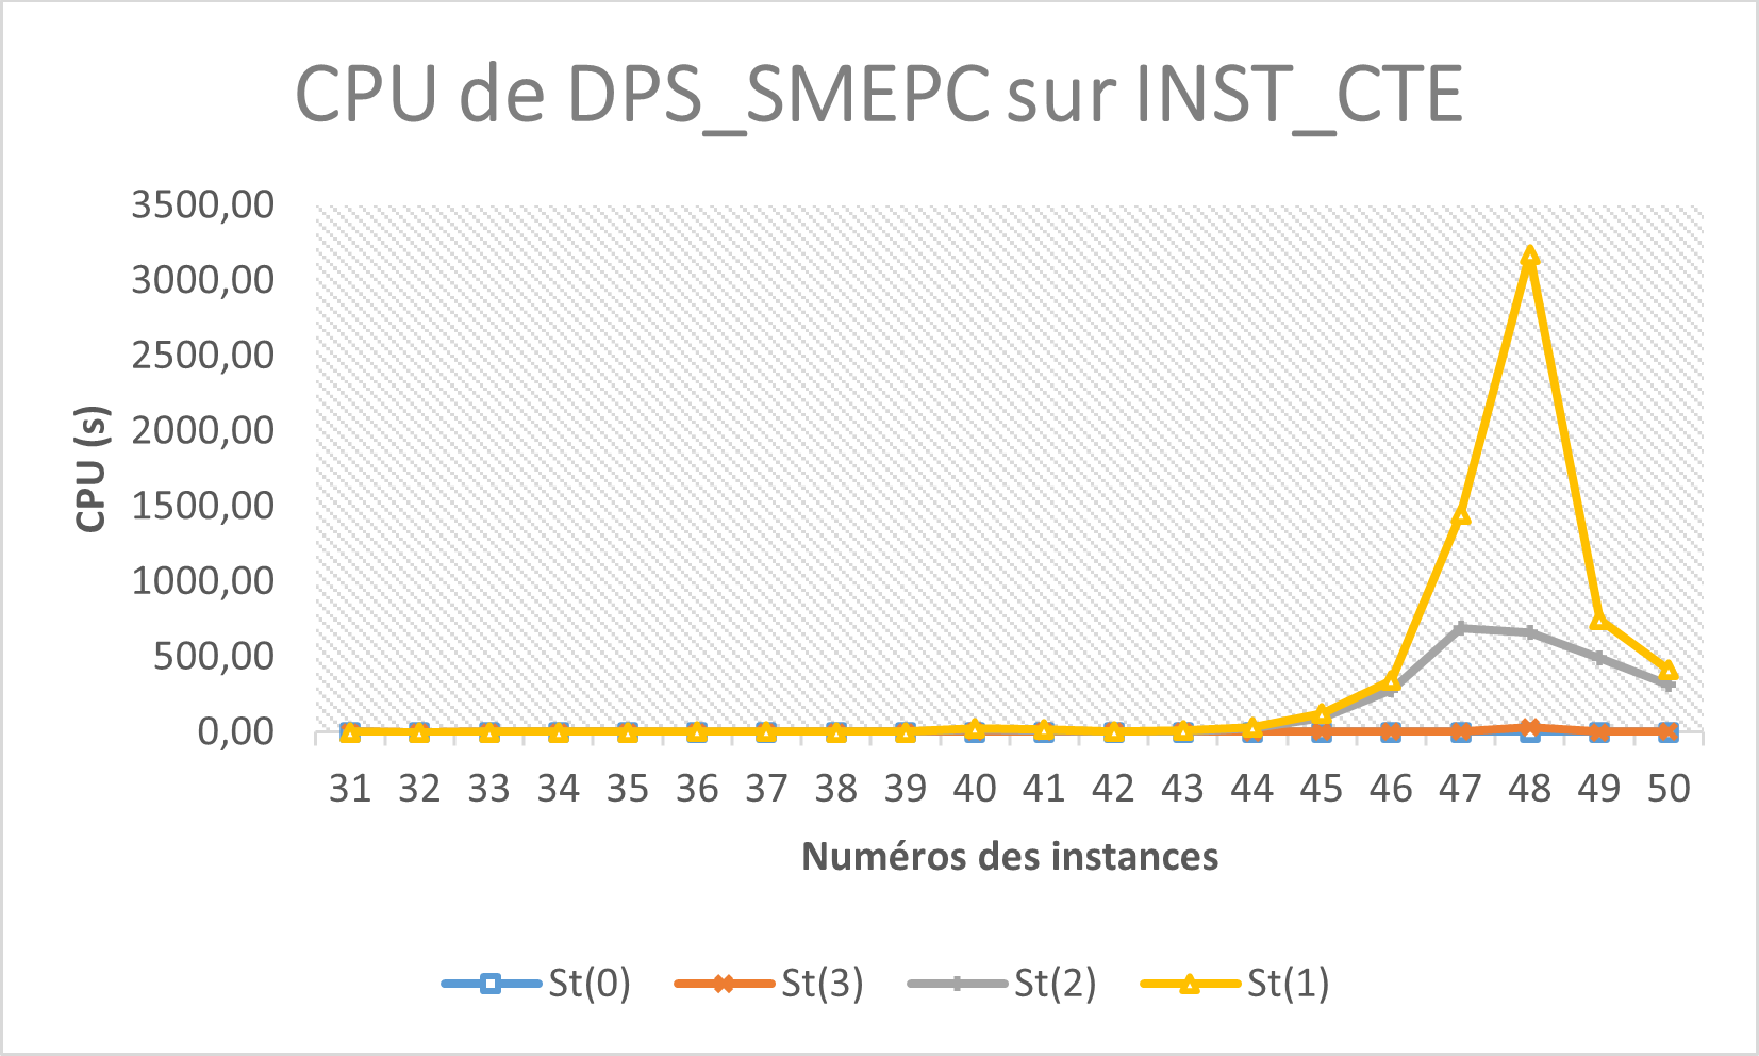
\includegraphics[width=9cm]{images_these/CPU_DPS_SMEPC_INST_CTE.pdf}&
		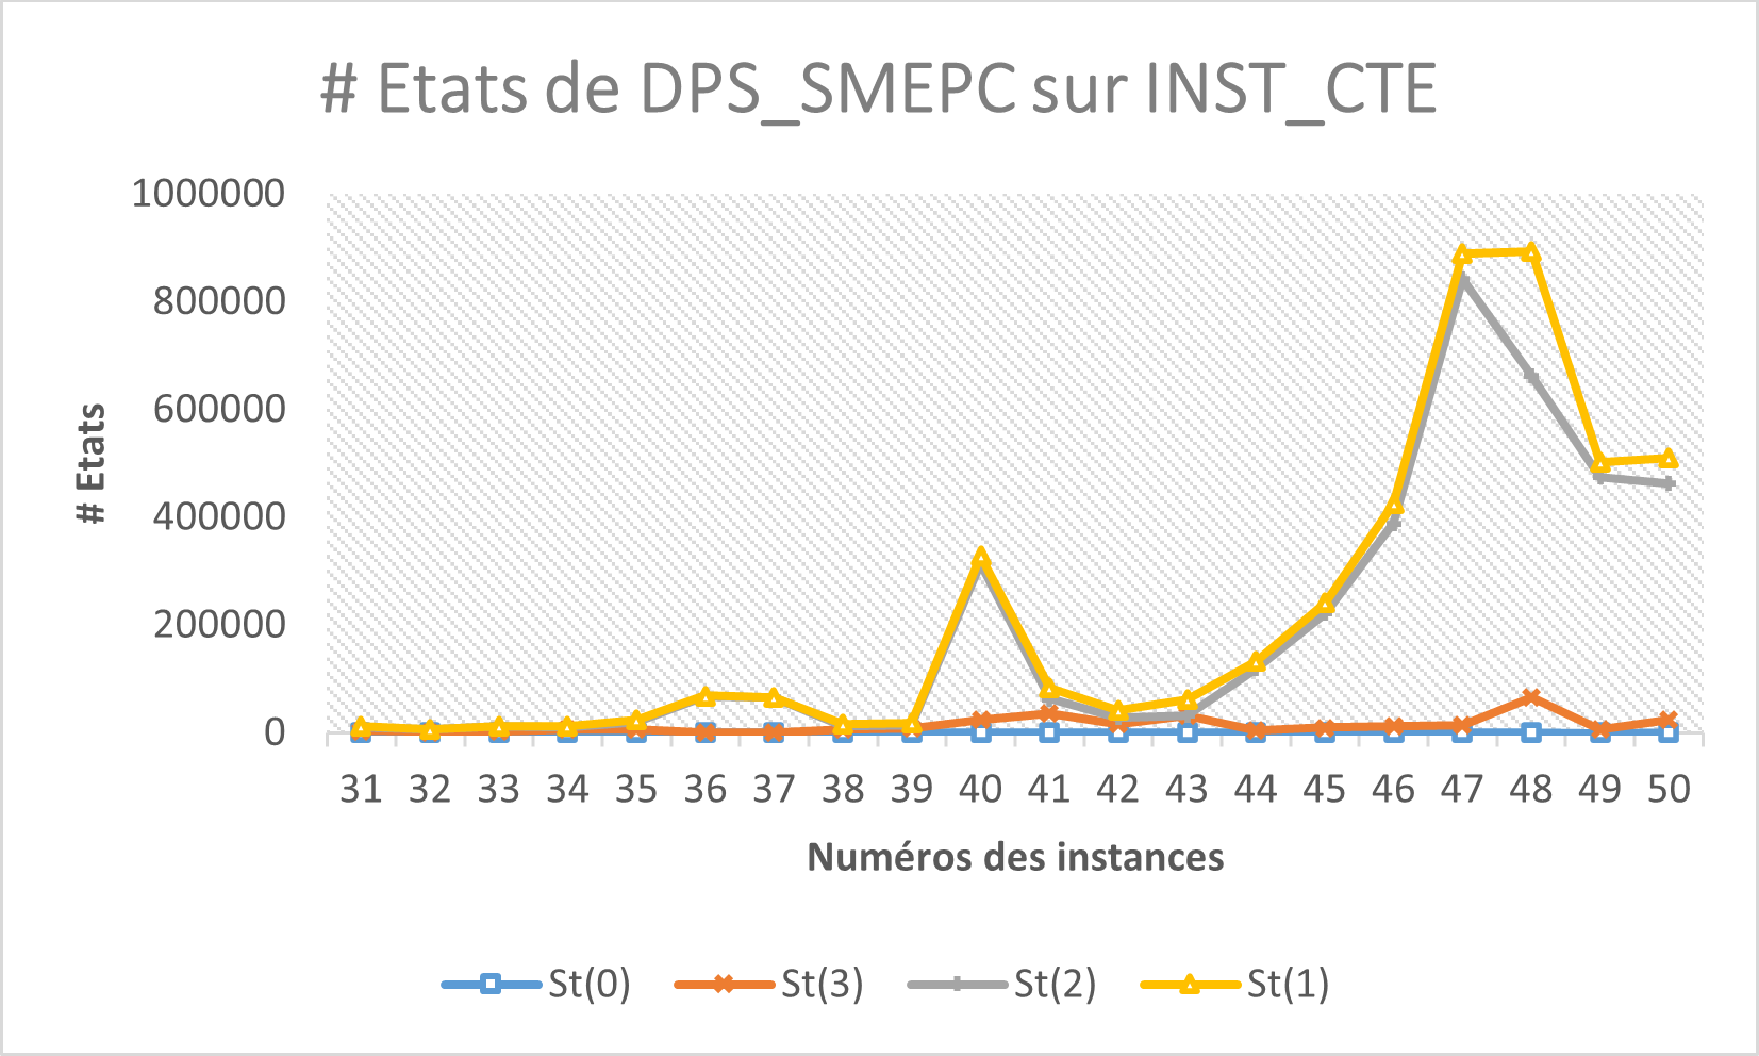
\includegraphics[width=9cm]{images_these/Etats_DPS_SMEPC_INST_CTE.pdf}
		\\
		(a) & (b)
	\end{tabular}
	\caption[Représentation graphique du CPU et du gap du tableau (\ref{power_filter2})]{Représentation graphique du tableau (\ref{power_filter2}). (a) représente le temps CPU et (b) représente le nombre d'états de chaque instance de INST\_CTE.}\label{gap_cpu_dps_smepc_INST_CTE}
\end{figure}
\section{Conclusion}
Nous avons présenté dans ce chapitre un schéma de programmation dynamique qui résout un problème d'ordonnancement qui nécessite de synchroniser les tâches effectuées par des véhicules avec un processus de production d'énergie. En raison du projet IMOBS3, nous traitons ici de la gestion synchrone, d'une part, d'une flotte de petits véhicules électriques équipés de piles à hydrogène et, d'autre part, d'une micro-usine chargée de la production locale de carburant à base d'hydrogène. Pris dans son ensemble, le problème concerne la prévision, la gestion de la sécurité et la programmation. Toutefois, comme notre objectif dans ce chapitre était de nous concentrer sur les caractéristiques algorithmiques de la synchronisation, nous nous sommes limités à ce dernier point et nous avons établit un modèle simplifié de production et de consommation d'énergie (SMEPC), limité au cas d'un véhicule devant effectuer des tâches selon un ordre préétabli tout en retournant périodiquement à la micro-usine pour faire le plein. La micro-usine a ses propres restrictions de production/stockage, et notre objectif était de synchroniser à la fois la micro-usine et le véhicule. Ce modèle est NP-Hard, et sa formulation linéaire est mal adaptée au traitement numérique. Nous l'avons abordé ici selon un paradigme purement centralisé, et nous avons présenté un schéma de programmation dynamique (DPS), qui met en œuvre la synchronisation tout en reliant les espaces temporels de la production et du véhicule. Nous avons enrichi ce DPS de mécanismes de filtrage exacts et heuristiques et il en ressort que le filtrage exact le plus efficace est le mécanisme de filtrage par estimation optimiste.

Ce DPS nous a fait énoncer un résultat PTAS (Polynomial Time Approximation Scheme) et fournir des solutions optimales. %en cas d'instances \textbf{SMEPC} pas trop importantes.
 %Il n'en reste pas moins que le temps de calcul reste coûteux.
  De plus, nous constatons que l'intégration complète des véhicules et de la production induit un manque de flexibilité qui rendra difficile la gestion des caractéristiques de collaboration dans les contextes de la vie réelle. Dans le prochain chapitre, nous changeons donc de paradigme et adoptons un point de vue qui consiste à aborder le \textbf{SMEPC} en émulant ces caractéristiques de collaboration : On divise notre modèle \textbf{SMEPC} en deux sous-modèles indépendants, l'un lié aux véhicules et l'autre à la micro-usine, que nous abordons tous les deux par le biais de DPS et que nous relions entre eux par une sorte d'interaction collaborative entre le demandeur et le producteur. De nombreuses questions restent à résoudre à l'instar de comment étendre notre approche à plusieurs véhicules.
Le chapitre suivant sera donc consacré à la présentation d'un schéma collaboratif pour résoudre notre problème.


%********************************************************************
\section{Annexes}

\subsection{Démonstration du théorème \ref{approx_scheme_pol}}
\label{approx_scheme_pol_section}
Cette section présente la démonstration du théorème \ref{approx_scheme_pol}. :
	$K$ étant fixé, le \textbf{DPS\_SMEPC}(K) est polynomial en temps. En outre, pour toute valeur $\varepsilon > 0$, on peut choisir $K$ suffisamment grand de telle sorte que si le \textbf{SMEPC} admet une solution optimale avec la valeur $W^{Opt}$, alors \textbf{DPS\_SMEPC}(K) donne une solution qui est réalisable en ce qui concerne les valeurs initiales $(1 + \varepsilon/ 2)\times H_0$ et $(1 + \varepsilon/ 2)\times E_0$, les valeurs seuils $(1 +\varepsilon )\times C^{Tank}, (1 + \varepsilon)\times C^{Veh}$ et $(1 + \varepsilon)\times TMax$ et dont la valeur de coût $Current\_Value$ n'est pas supérieure à $W^{Opt}+ \varepsilon$.

%\textbf{Démonstration} :
$K$ étant fixé, le fait que l'algorithme \textbf{DPS\_SMEPC}(K) soit polynomial en temps provient du fait que $TMax$, $C^{Tank}$ et $C^{Veh}$ sont censés être limités par des fonctions polynomiales de $N$ et $M$ : le nombre de triplets possibles $(s, W, Father)$ dans la liste $S(i, j)$ que nous traitons à chaque itération de la boucle principale est limité par une fonction polynomiale de $N$, $M$ et la taille de codage de $TMax$, $C^{Tank}$ et $C^{Veh}$. 

De la même manière, étant donné $\varepsilon$, on voit que si $K$ est suffisamment grand, alors l'erreur relative $(Round^*(TMax, K) - TMax) / TMax$ induite par le remplacement de $TMax$ par $Round^*(TMax, K)$ ne dépasse pas $\varepsilon$. Il en va de même pour les capacités $C^{Veh}$ et $ C^{Tank}$. 

Afin de réaliser la preuve du théorème \ref{FPTAS_theo1}, nous devons maintenant envisager une solution optimale $Sol^{Opt}$, donnée avec sa valeur $W^{Opt}$. La solution $Sol^{Opt}$ peut être associée à une séquence de dates $(i_h, j_h)$, $h = 0, \dots, H \leq N + M$, une séquence d'états $s_0, s_1, \dots, s_H$, avec la valeur $W_0, \dots, W_H$, et une séquence de décisions $D_0, \dots, D_{H-1}$, qui induit des transitions $((i_h, j_h) , s_h) \rightarrow ((i_{h + 1}, j_{h + 1}) , s_{h + 1})$, $h = 0, \dots, H - 1$, et de vérifier que si $K$ est suffisamment grand, \textbf{DPS\_SMEPC}(K) calcule une solution $Current\_Sol$ qui est réalisable par rapport aux valeurs seuils $(1 + \varepsilon)\times C^{Tank}, (1 + \varepsilon )\times C^{Veh} et (1 + \varepsilon)\times TMax$ et dont la valeur de coût $Current\_Value$ n'est pas supérieure à $W^{Opt} + \varepsilon$. Pour ce faire, on fixe $K$ et on prouve par induction sur $h$ que, pour tout $h = 0, \dots, H$,
Il existe dans l'ensemble $S(i_h, j_h)$ calculé par le \textbf{DPS\_SMEPC}(K) quelque triplet $(s = (Z, T, V^{Tank} , V^{Veh}), W, Father)$ de sorte que, si on a $s_h = (Z_h, T_h, V^{Tank}_h, V^{Veh}_h)$ :	
%	\begin{itemize}[label=$\square$]
%		\item $W\leq W_h$ ;
%		\item $Z_h=Z$ ;
%		\item $ T\leq T_h \times (1+h\times 2^{-K}/(N+M))$;
%		\item $V^{Tank}\times (1+h\times 2^{-K}/2\times (N+M)) \leq V^{Tank}_h \leq V^{Tank} \times (1+h\times 2^{-K}/(N+M))$; 
%		\item $V^{Veh} \times (1+h\times 2^{-K}/2\times (N+M)) \leq V^{Veh}_h  \leq V^{Veh}_h\times (1+h\times 2^{-K}/(N+M))$
%	\end{itemize}

\begin{subequations}
	\begin{align}
	\label{22}	W\leq W_h&  & \\ 
	\label{23}	Z_h=Z&  & \\
	\label{26}	T\leq T_h \times (1+h\times 2^{-K}/(N+M))&  & \\
	\label{24}	V^{Tank}\times (1+h\times 2^{-K}/2\times (N+M)) \leq V^{Tank}_h \leq V^{Tank} \times (1+h\times 2^{-K}/(N+M))&  &\\
	\label{25}	V^{Veh} \times (1+h\times 2^{-K}/2\times (N+M)) \leq V^{Veh}_h  \leq V^{Veh}\times (1+h\times 2^{-K}/(N+M))&  & 
	\end{align}
\end{subequations}

Nous supposons que c'est vrai pour un $h$ donné et essayons d'appliquer la décision $D_h$ à l'état $s_h$. Nous déduisons des équations (\ref{23}) et (\ref{26}) que l'application de $D_h$ respectera le seuil $Round^*(TMax, K)$. A cause de l'équation (\ref{24}), $D_h$ ne rendra pas la quantité d'hydrogène dans la micro-usine négative ou ne dépassera pas le $Round^*(C^{Tank}, K)$. De même, (\ref{25}) implique que $D_h$ ne fera pas en sorte que la quantité d'hydrogène dans le véhicule soit négative ou dépasse le $Round^*(C^{Veh}, K)$. Il s'ensuit que cette décision va être réalisable. Nous voyons alors que l'état $s' = (Z', T', V'^{Tank}, V'^{Veh})$ résultant à la valeur temporelle $(i_{h+1}, j_{h+1})$ de l'application de $D_h$ à l'état $s$ et à la valeur $W'$ correspondante sera tel que :		

\begin{subequations}
	\begin{align}
	\label{27}	W' \leq W_{h+1}&  & \\ 
	\label{28}	Z_{h+1}=Z'&  & \\
	\label{29}	T'\leq T_{h+1} \times (1+h\times 2^{-K}/(N+M))&  & \\
	\label{30}	V'^{Tank}\times (1+h\times 2^{-K}/2\times (N+M)) \leq V^{Tank}_{h+1} \leq V'^{Tank} \times (1+h\times 2^{-K}/(N+M))&  &\\
	\label{35}	V'^{Veh} \times (1+h\times 2^{-K}/2\times (N+M)) \leq V^{Veh}_{h+1}  \leq V'^{Veh}\times (1+h\times 2^{-K}/(N+M))&  & 
	\end{align}
\end{subequations}
Mais (\ref{28}, \ref{29}, \ref{30}, \ref{35}) combiné avec les mécanismes de propagation liées aux erreurs relatives impliquent que si $(s^*, W^*, Father^*)$ est l'élément équivalent à $(s', W')$ modulo les $K + L$ plus grands bits qui restent dans $S(i_{h + 1}, j_{h + 1})$ du \textbf{DPS\_SMEPC}(K), alors nous avons : 	

\begin{subequations}
	\begin{align}
	\label{31}	W^* \leq W_{h+1}&  & \\ 
	\label{32}	Z_{h+1}=Z^*&  & \\
	\label{33}	T^*\leq T_{h+1} \times (1+(h+1)\times 2^{-K}/(N+M))&  & \\
	\label{34}V^{Tank*}\times (1+(h+1)\times 2^{-K}/2\times (N+M)) \leq V^{Tank}_{h+1} \leq V^{Tank*} \times (1+(h+1)\times 2^{-K}/(N+M))&  &\\
	\label{36}V^{Veh*} \times (1+(h+1)\times 2^{-K}/2\times (N+M)) \leq V^{Veh}_{h+1}  \leq V^{Veh*}\times (1+(h+1)\times 2^{-K}/(N+M))&  & 
	\end{align}
\end{subequations}%
Nous déduisons que les équations (\ref{23}, \ref{26}, \ref{24}, \ref{25}) sont vraies pour tout $h=0, \dots, H$. Cela nous permet de choisir $K$ de telle manière que $2K$ est plus grand que $(N + M + 1) / \varepsilon$.  $\square$

